\chapter{Health as Human Capital}

\fancyhead[L]{ECON0024}
\fancyhead[C]{Ch.3 Health as Human Capital}
\fancyhead[R]{Kuangjie Ni}
\fancyfoot[L]{\hyperlink{tableofcontents}{Back to Table of Contents}}
\fancyfoot[R]{Kuangjie Ni}

\section{Intro: Why are some of us less healthy than others?}

    \begin{itemize}
        \item Bad genes
        \item Bad lifestyles
        \item Poor healthcare 
        \item Poor early environment 
        (e.g. poor parenting, mum drinking during pregnancy)
   \end{itemize}    

\section{Health Spending}

    \subsection{Facts about Health Spending: Global}

        \subsubsection{Health spending per capita}

            \begin{figure}[H]
                \centering
                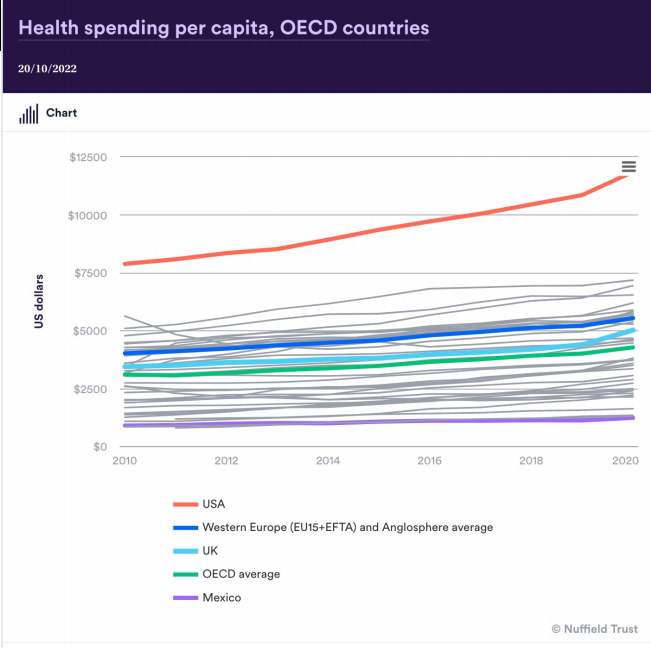
\includegraphics[width=3in]{images/ch3/1 Health spending OECD.png}
                \caption{Health Spending per Capita, OECD countries}
            \end{figure}
            \begin{itemize}
                \item Health spending per capita is increasing over time. People are living longer than they used to be. The longer you live, the sicker you get and the more money you spend on healthcare. 
                \item US has a higher health spending and a particular healthcare structure.
            \end{itemize}
        
        \subsubsection{A Large Fraction Is Government/Compulsory Spending}
            \begin{figure}[H]
                \centering
                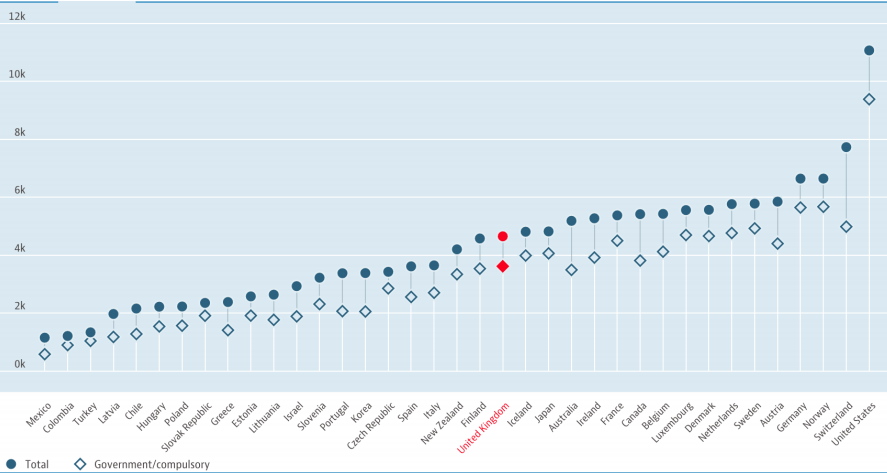
\includegraphics[width=5in]{images/ch3/2 Government.png}
                \caption{Health spending: Total including government/compulsory spending in US dollars/capita, 2019}
            \end{figure}      
            \begin{itemize}
                \item Blue dots are the total health spending, and diamonds are the government/compulsory spending. 
                \item US government spends a lot of money on healthcare.
            \end{itemize}
        
        \subsubsection{Total Spending as \% of GDP}
            \begin{figure}[H]
                \centering
                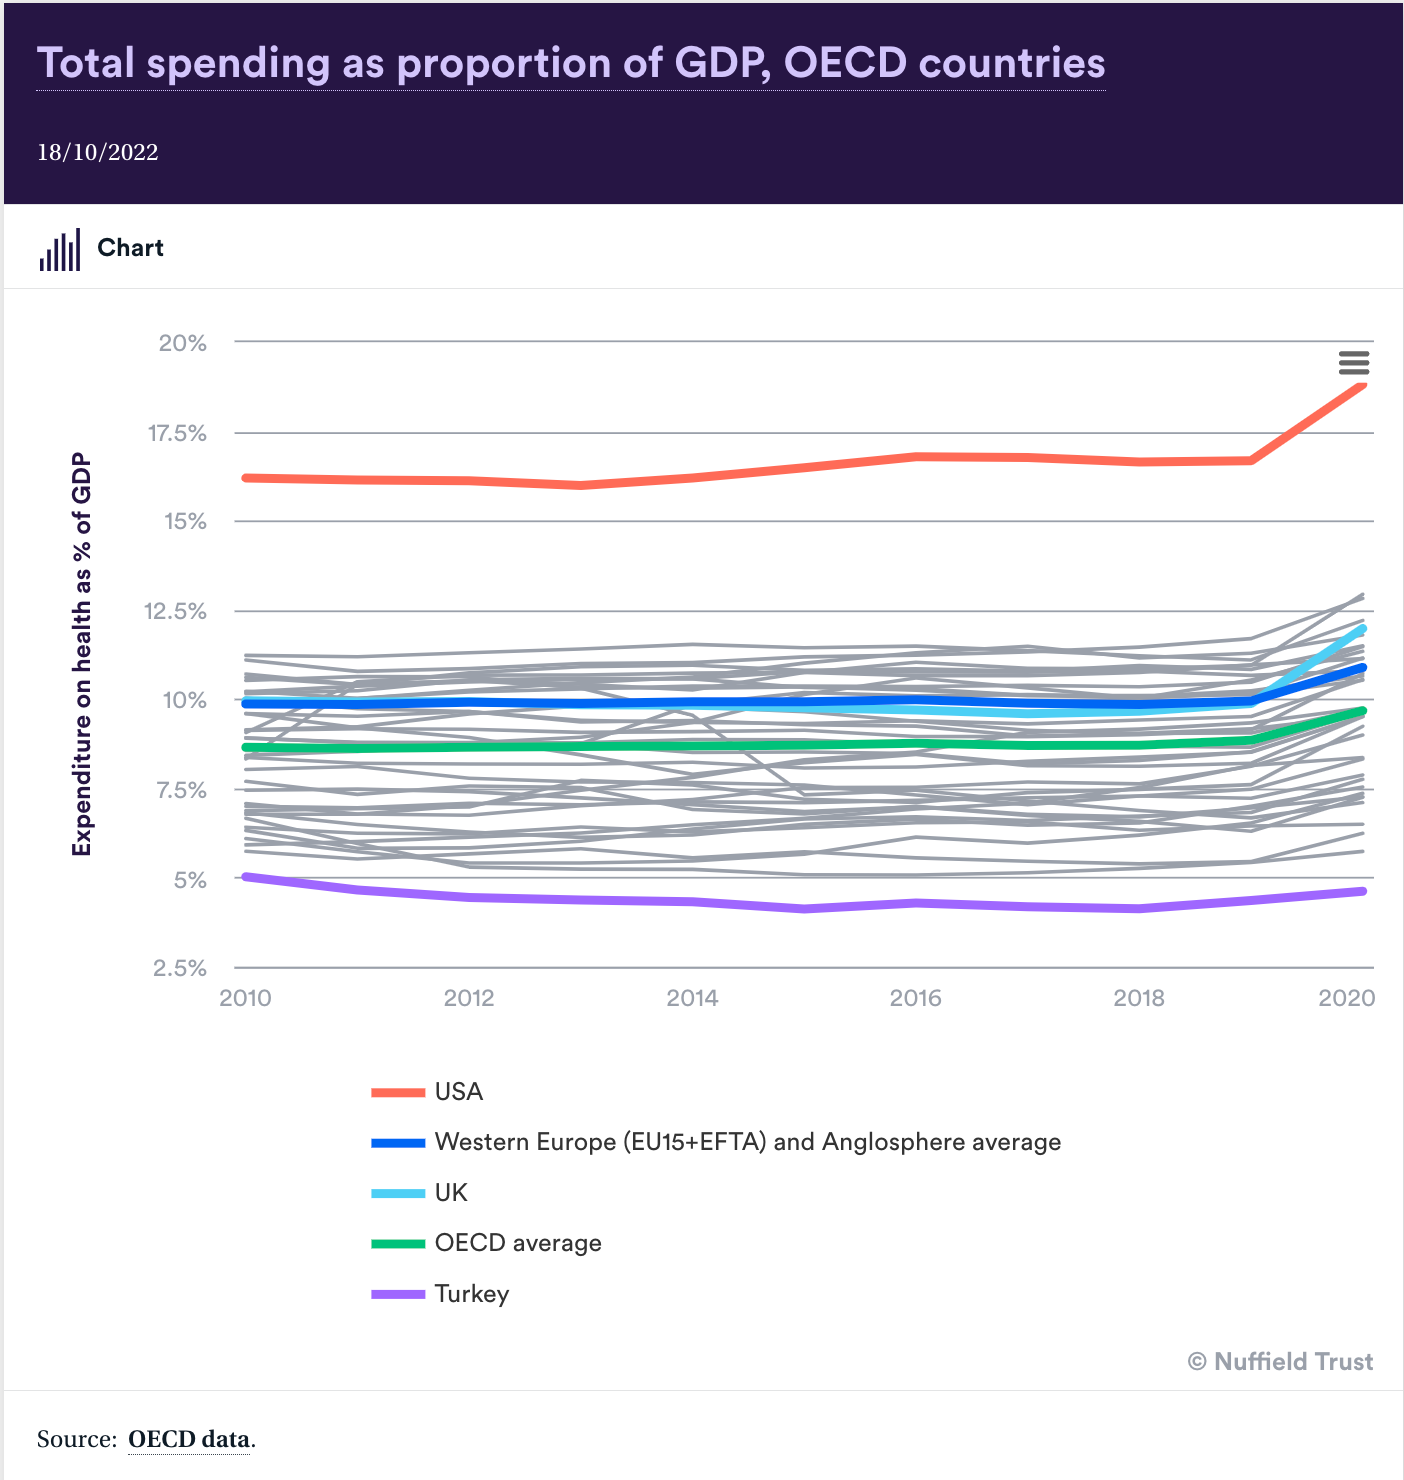
\includegraphics[width=4in]{images/ch3/3 GDP.png}
                \caption{Total spending as a proportion of GDP, OECD countries}
            \end{figure}            
            \begin{itemize}
                \item US has the highest health spending as a proportion of GDP.
                \item The total health spending as a proportion of GDP increased during the pandemic.
            \end{itemize}
        
    \subsection{Facts about Health Spending: the UK}
    
        \subsubsection{Health as \% of UK Total Spending}  
            \begin{figure}[H]
                \centering
                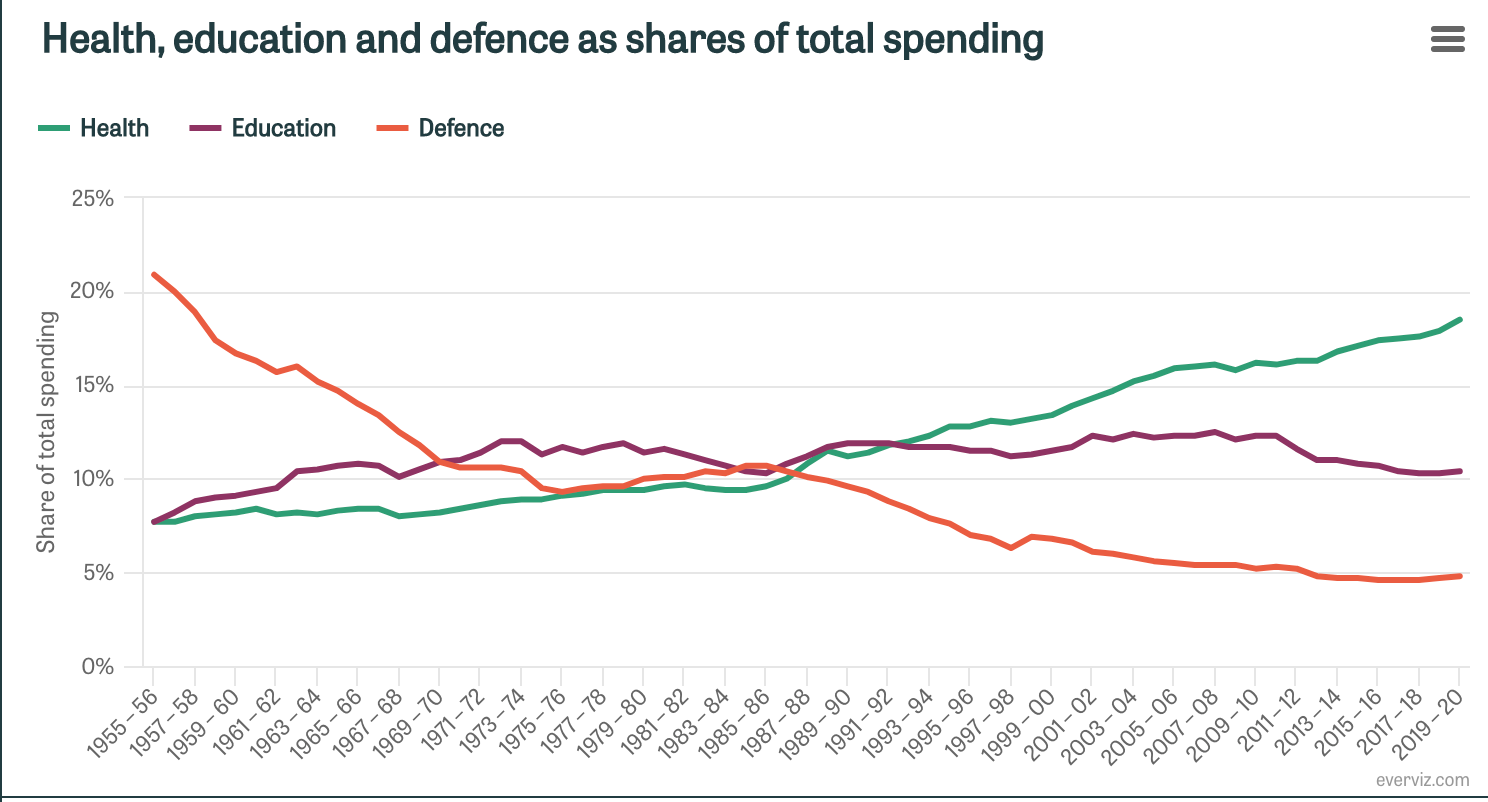
\includegraphics[width=4in]{images/ch3/4.png}
                \caption{Health, education and defence as shares of total spending}
            \end{figure} 
        \begin{itemize}           
            \item Health spending takes a bigger share of total UK spending over the last 70 years.
            \item The share of education spending is approximately flat, and the share of defence spending declines significantly.
        \end{itemize}
        
        \subsubsection{Components of UK Government Spending}  
            \begin{figure}[H]
                \centering
                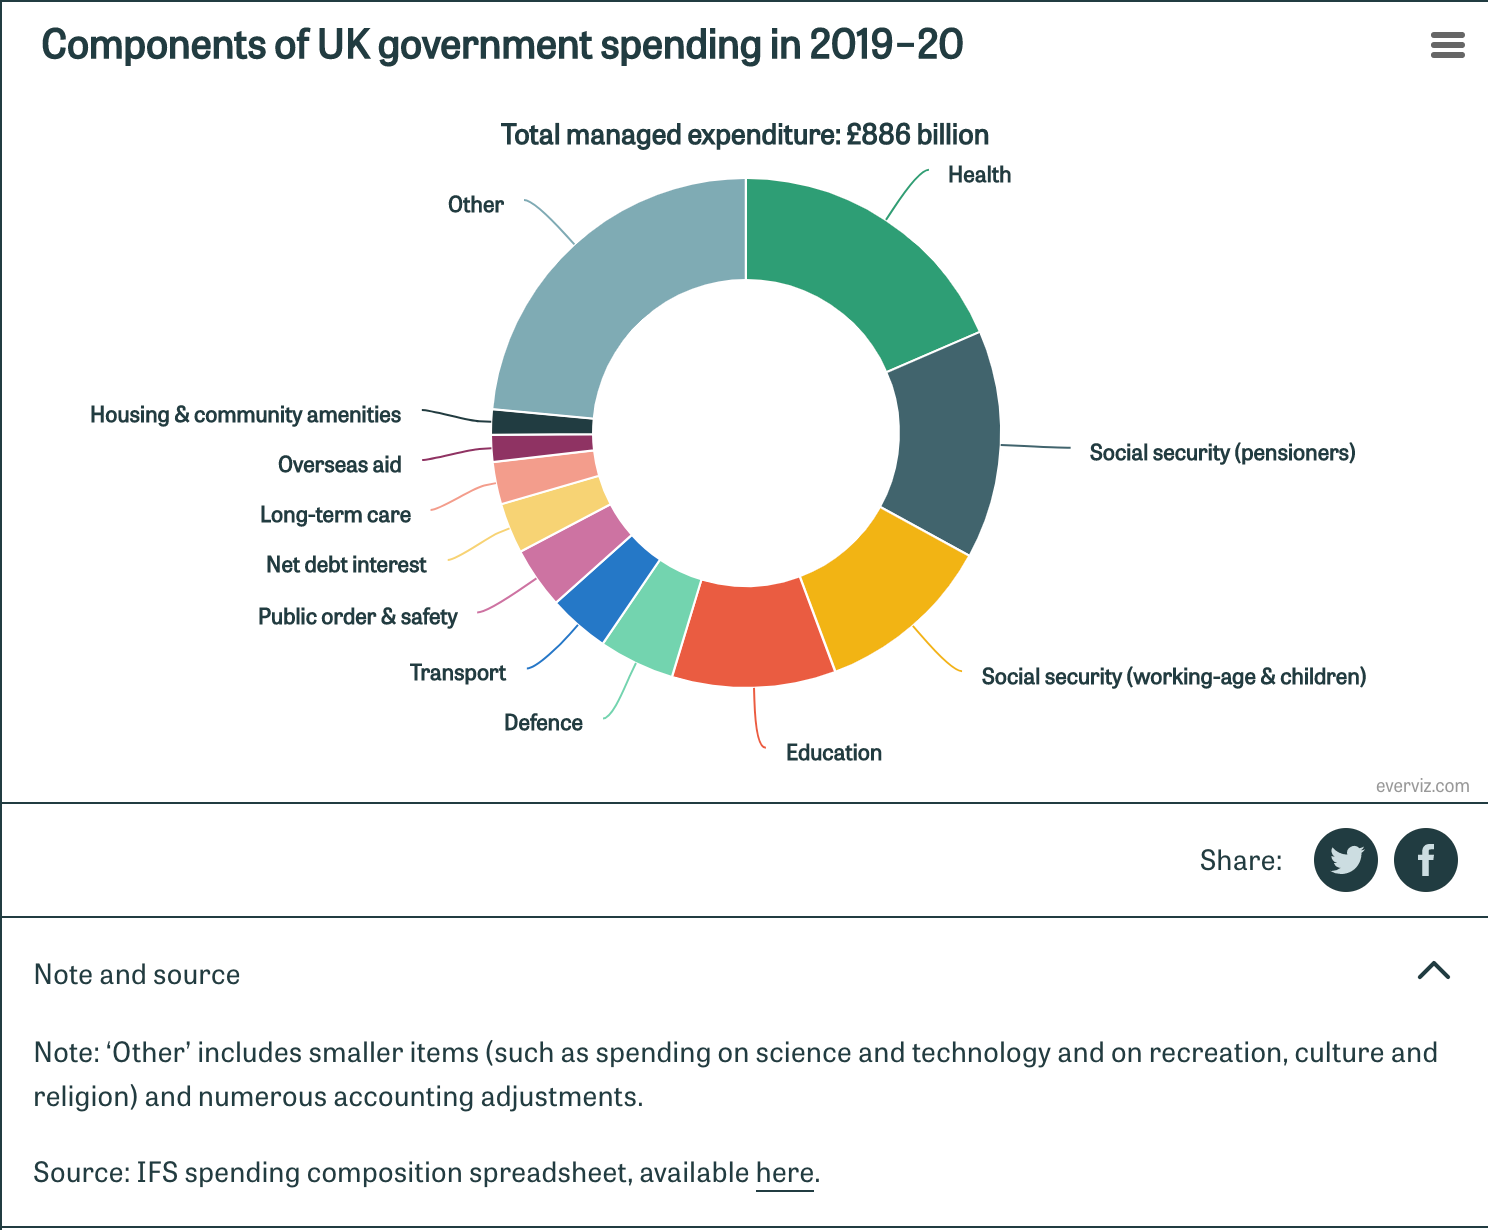
\includegraphics[width=4in]{images/ch3/5.png}
                \caption{Components of UK GOV spending in 2019-20}
            \end{figure} 
            Total managed UK government expenditure is 886 billion pounds, and health spending is a very important component.

        \subsubsection{UK Public Spending on Health}         
            \begin{figure}[H]
                \centering
                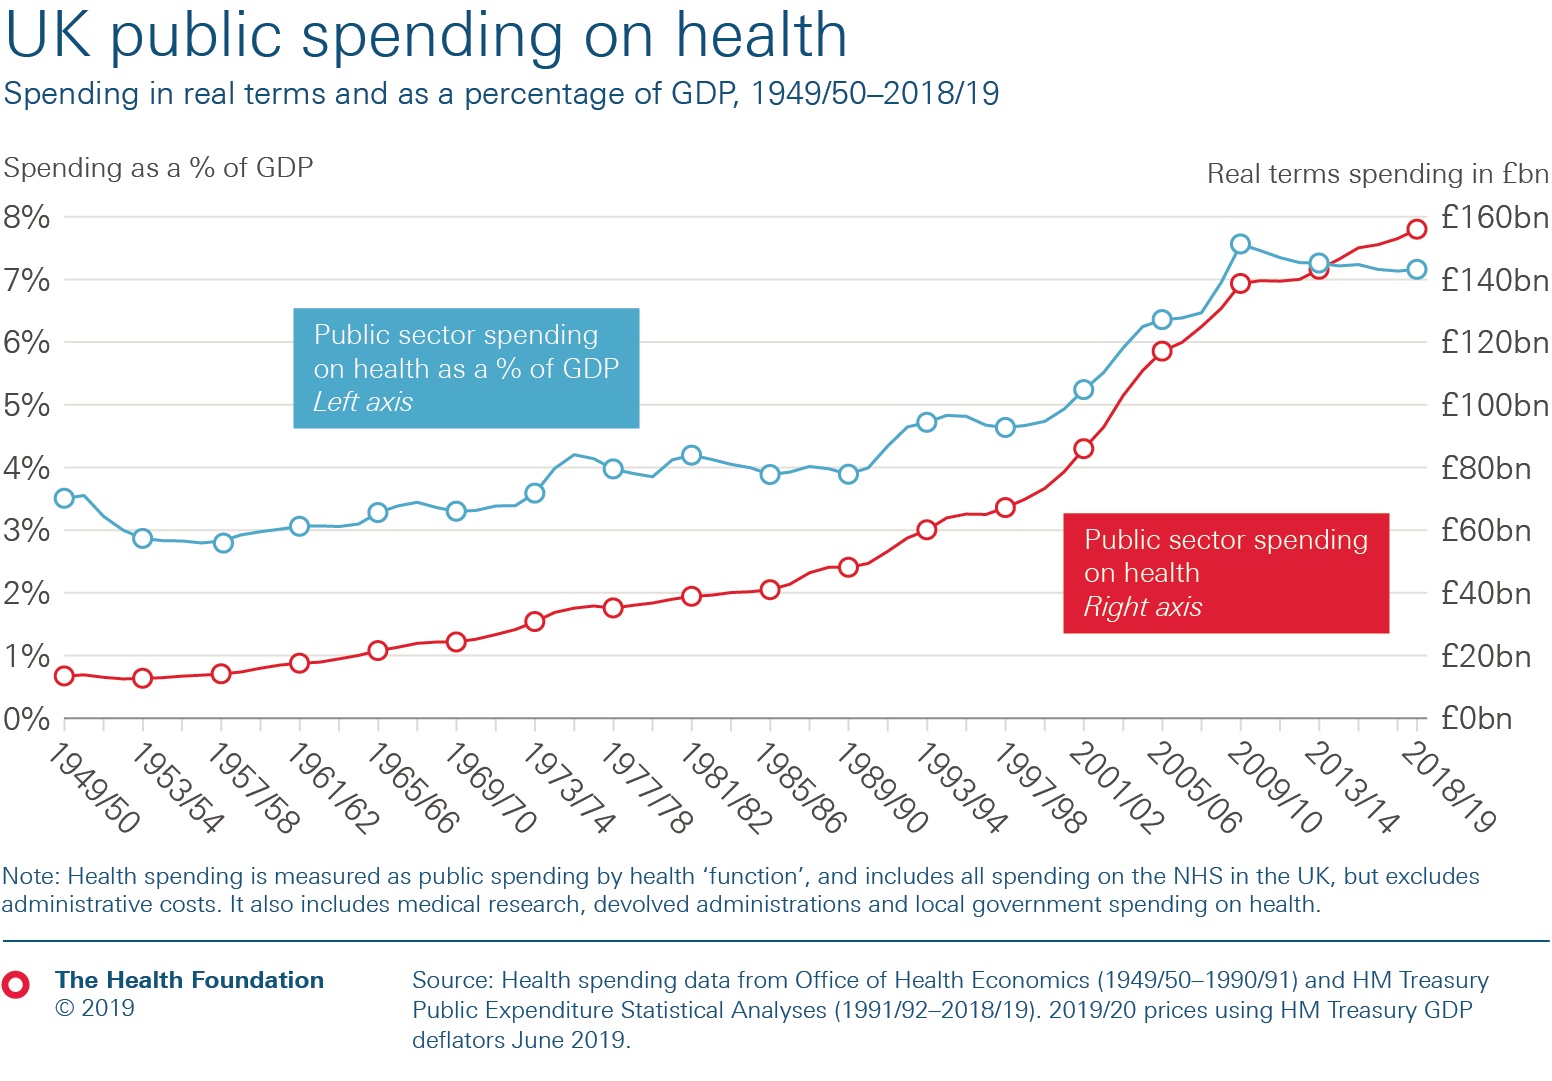
\includegraphics[width=4in]{images/ch3/6.png}
                \caption{UK public spending on health, 1949/50 - 2018/19}
            \end{figure} 
            \begin{itemize}           
                \item The blue line shows the UK public sector spending on health as a percentage of GDP (left axis). The red line shows the UK public sector spending on health in real terms (right axis).
                \item The UK public sector spending on health has increased both as a percentage of GDP and in real terms since the end of World War II.
            \end{itemize}

        \subsubsection{Department of Health and Social Care spending} 
            \begin{figure}[H]
                \centering
                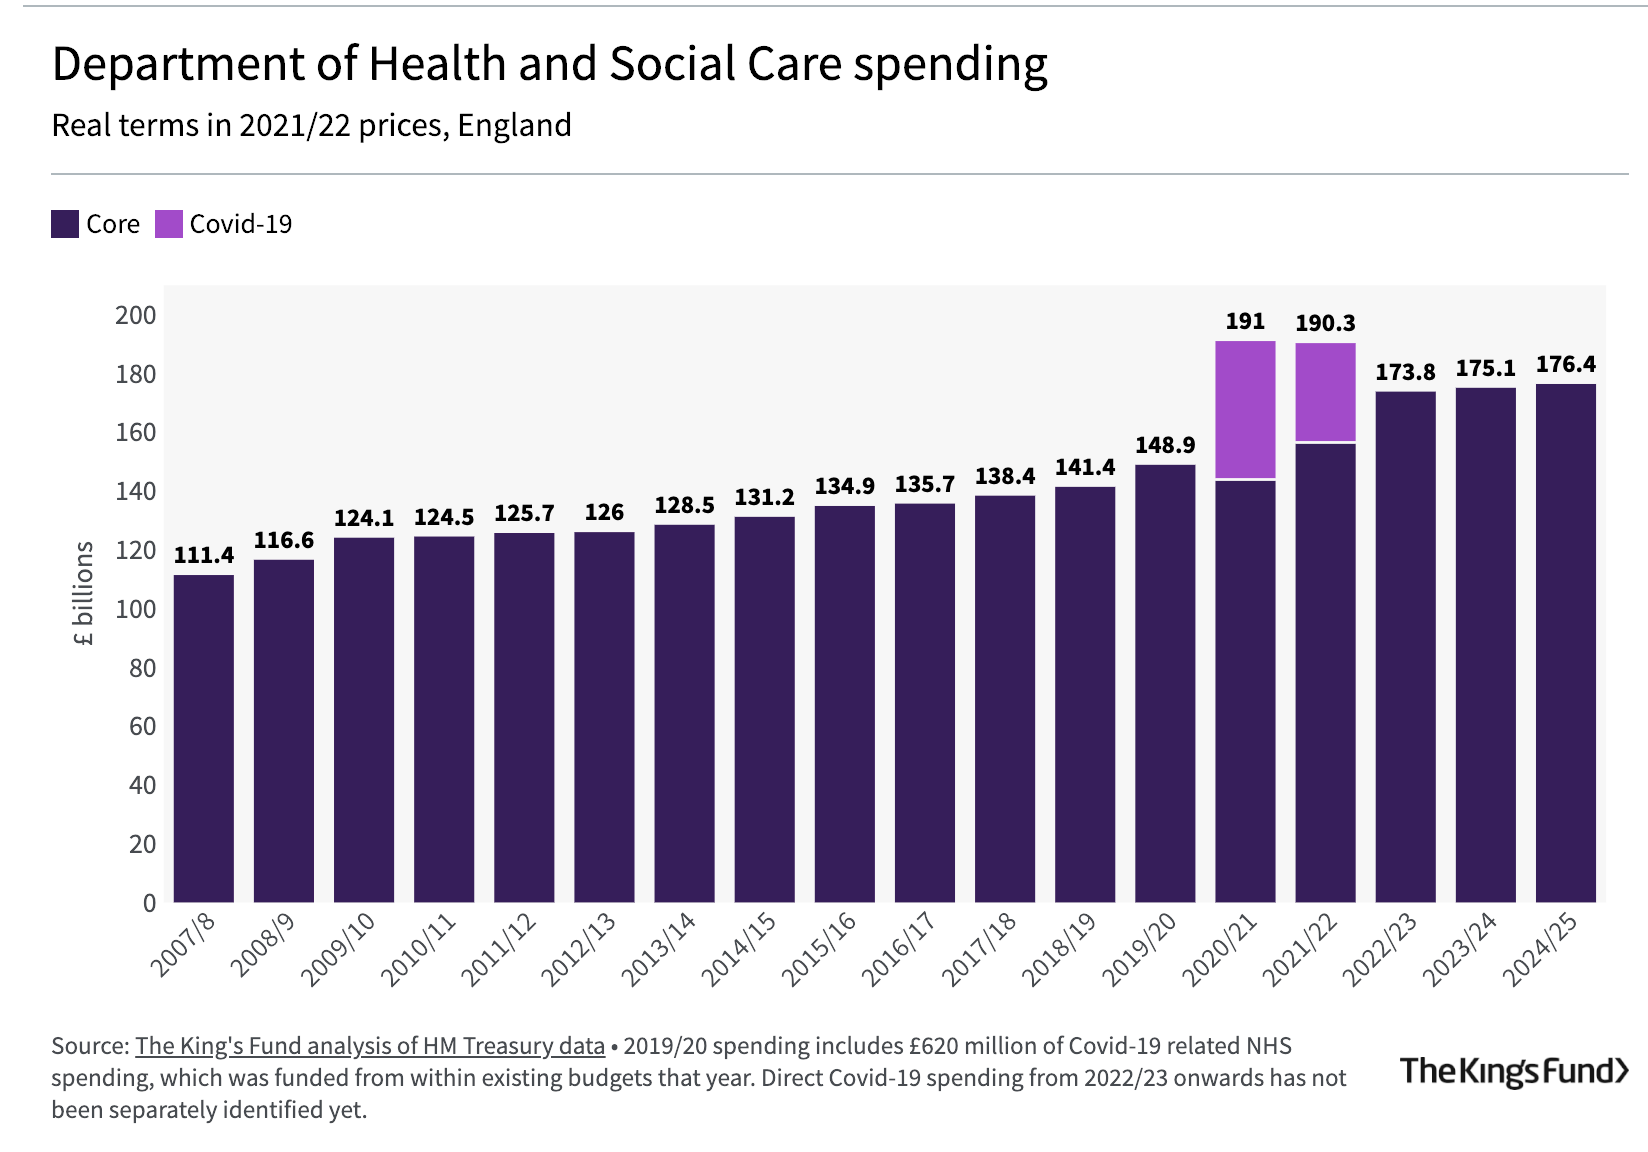
\includegraphics[width=4in]{images/ch3/7.png}
                \caption{Department of Health and Social Care spending, real terms in 2021/22 prices, England}
            \end{figure} 
                The Department of Health and Social Care spending increased a lot due to Covid-19, and the core spending keeps going up after 2021/22.

        \subsubsection{UK Health Spending Growth} 
            \begin{figure}[H]
                \centering
                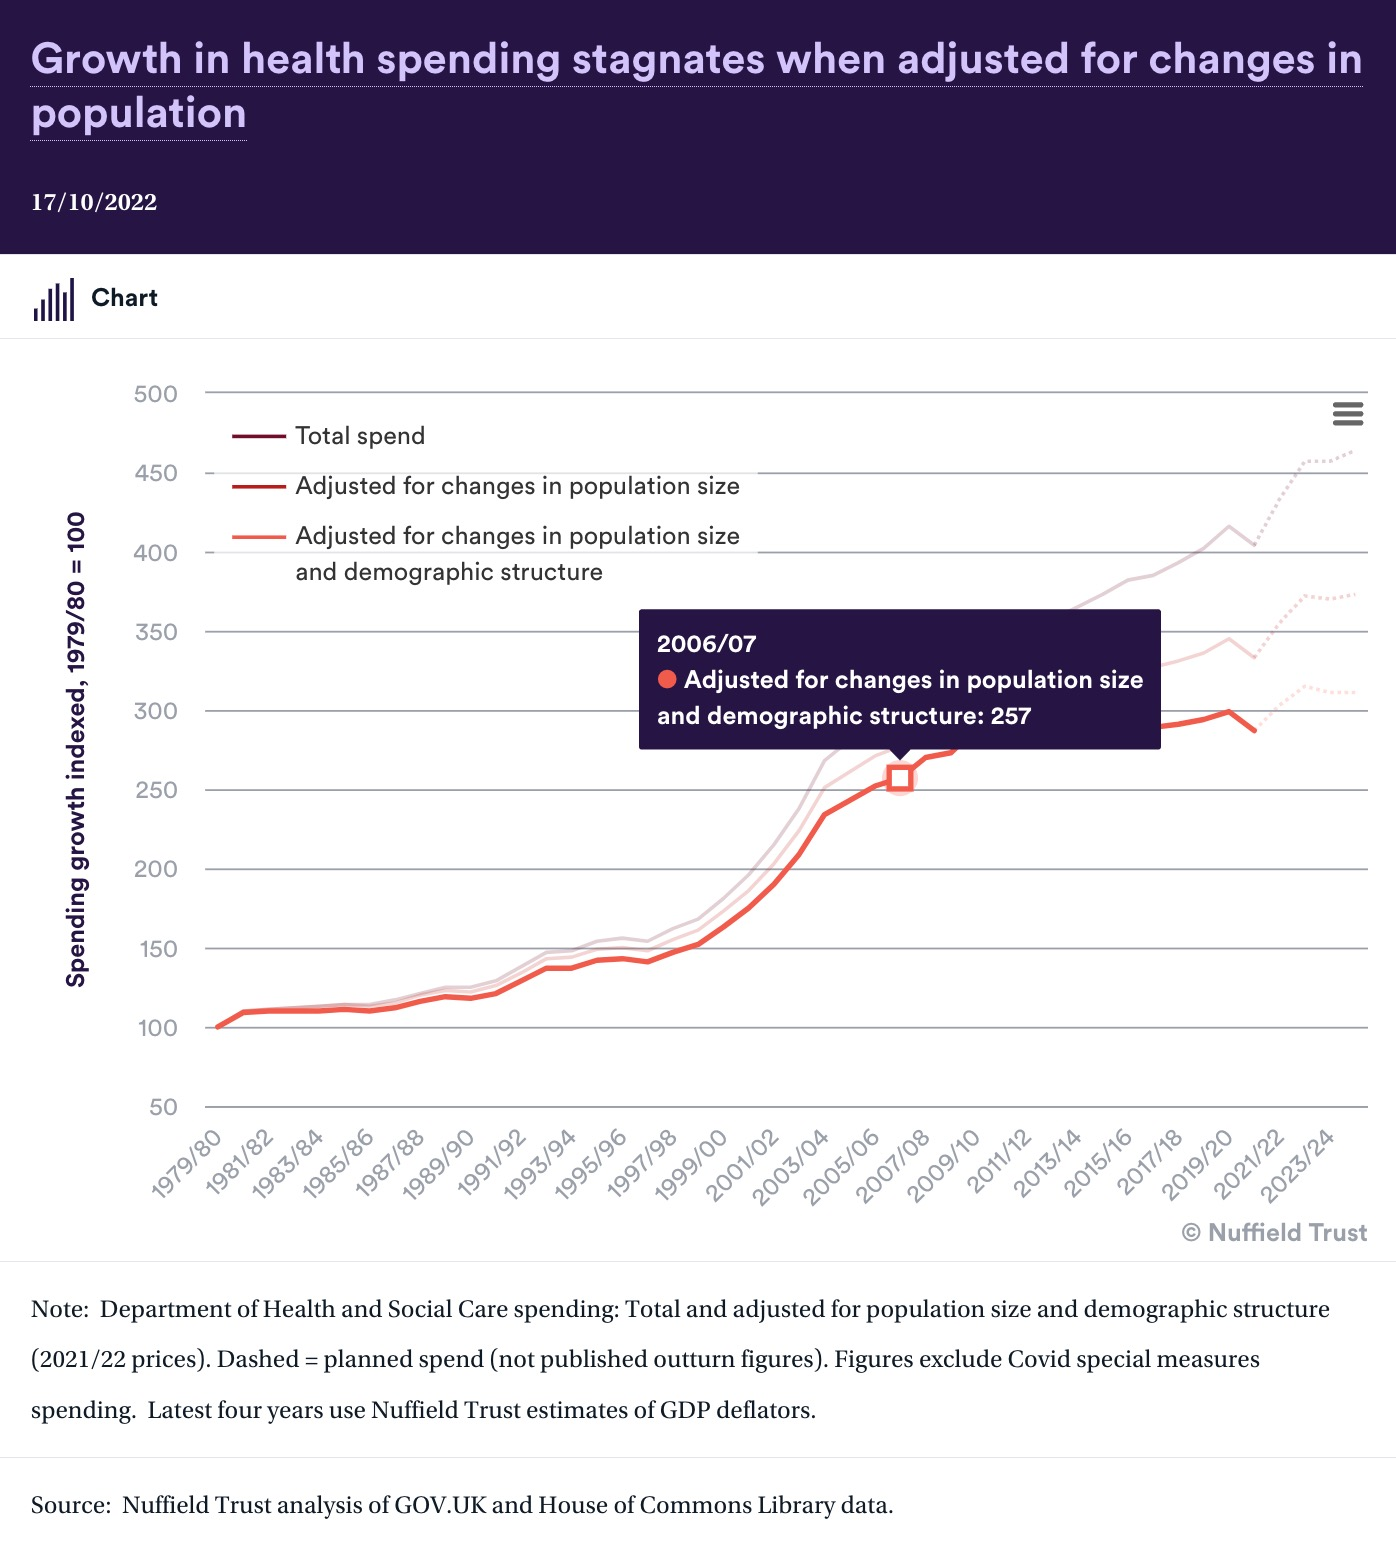
\includegraphics[width=4in]{images/ch3/8.png}
                \caption{Health spending growth indexed, 1979/80 = 100}
            \end{figure} 
            \begin{itemize}           
                \item The dark red line shows the total health spending. The red line shows the total health spending adjusted for changes in population size. The orange line shows the total health spending adjusted for changes in population size and demographic structure.
                \item Growth in health spending stagnates after adjusted for changes in population (population ageing).
            \end{itemize}       
            \begin{figure}[H]
                \centering
                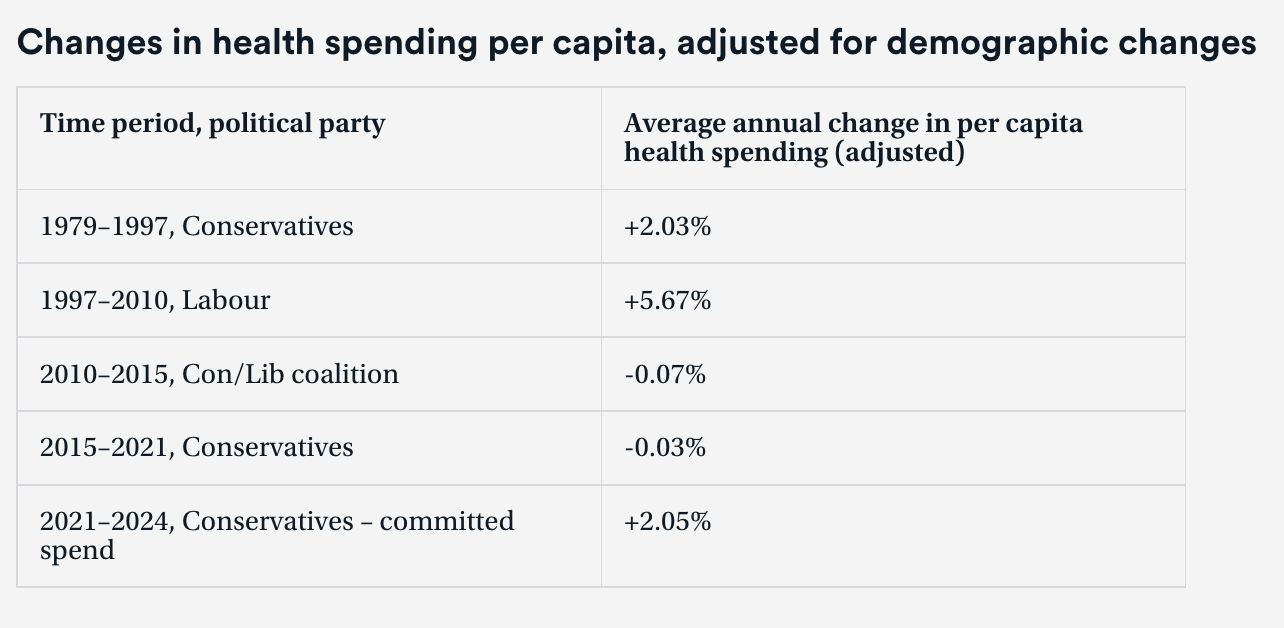
\includegraphics[width=4in]{images/ch3/9.png}
                \caption{Changes in health spending per capita, adjusted for demographic changes}
            \end{figure} 
            The Labour government has the highest increase in health spending per capita.

    \subsection{How Is the Health Budget Spent?}

        \subsubsection{}




        \subsubsection{How funding flows in the NHS?} 
            \begin{figure}[H]
                \centering
                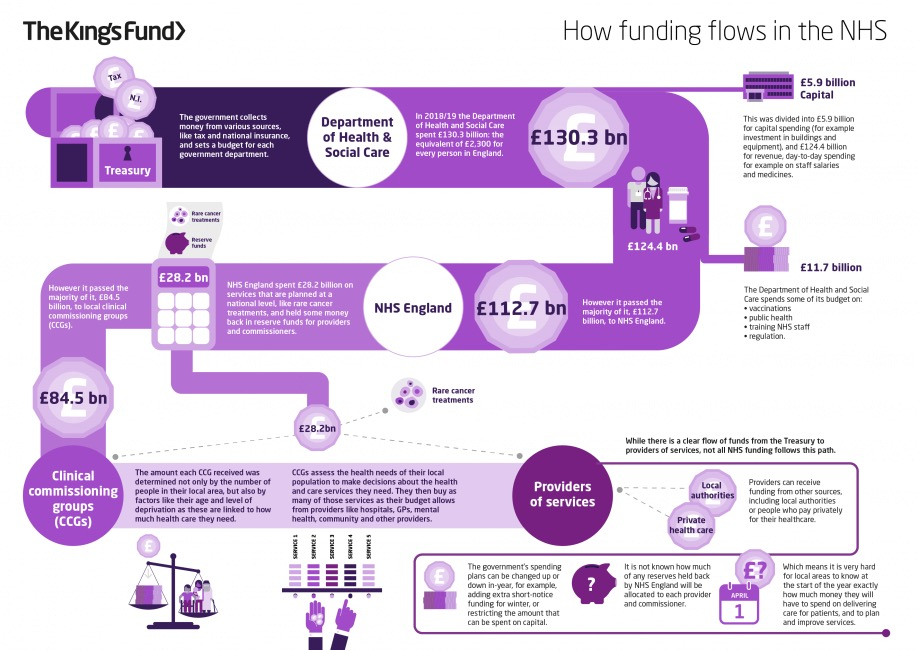
\includegraphics[width=5in]{images/ch3/11.png}
                \caption{How funding flows in the NHS?}
            \end{figure} 
            \begin{itemize}           
                \item In 2018/19, the Treasury gave the Department of Health and Social Care 130.3 billion pounds. This was divided into 5.9 billion for capital spending and 124.4 billion for day-to-day spending. 
                \item The 124.4 billion was further divided into 11.7 billion for preventive services (vaccinations, public health, training NHS staff, and regulation) and 112.7 billion for NHS England. 
                \item NHS England spent 28.2 billion on national-planned services, such as rare cancer treatments, and passed the remaining 84.5 billion to the clinical commissioning groups (CCGs). The amount each CCG received was determined by the number of people in the local area and by factors such as age (how sick they are).
            \end{itemize} 

        \subsubsection{Example: Bradford CCG}         
            \begin{figure}[H]
                \centering
                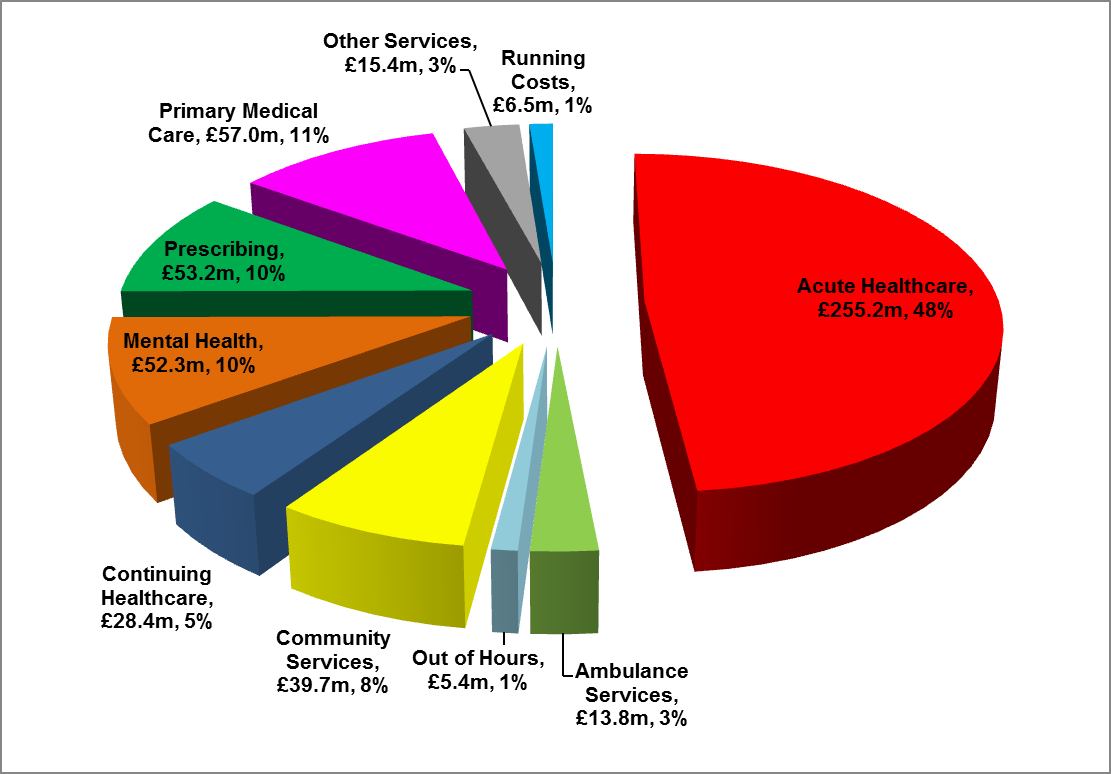
\includegraphics[width=4in]{images/ch3/12.png}
                \caption{Total CCG net expenditure, 2019/20(526.9 million pounds)}
            \end{figure} 
            Half of the money goes to acute healthcare. A small proportion of the money goes to preventive services, such as community services (health visitors and immunisation).
        
        \subsection{Preventive Care}
        
             \subsection{Other Factors that Matter to Health other than Healthcare} 
                \begin{figure}[H]
                    \centering
                    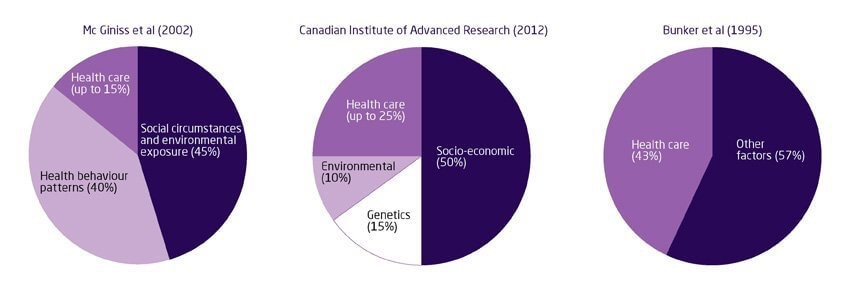
\includegraphics[width=5in]{images/ch3/14.png}
                    \caption{There is more to health than healthcare}
                \end{figure} 
                These three pie charts show the proportion of health that does not depend on the healthcare. Although the proportion varies between different studies, healthcare matters by less than a half in all studies.
    
            \subsubsection{Example: The role of lifestyles in the prevention of chronic conditions}         
            \begin{figure}[H]%option [H] means "strictly here"
                    \centering
                    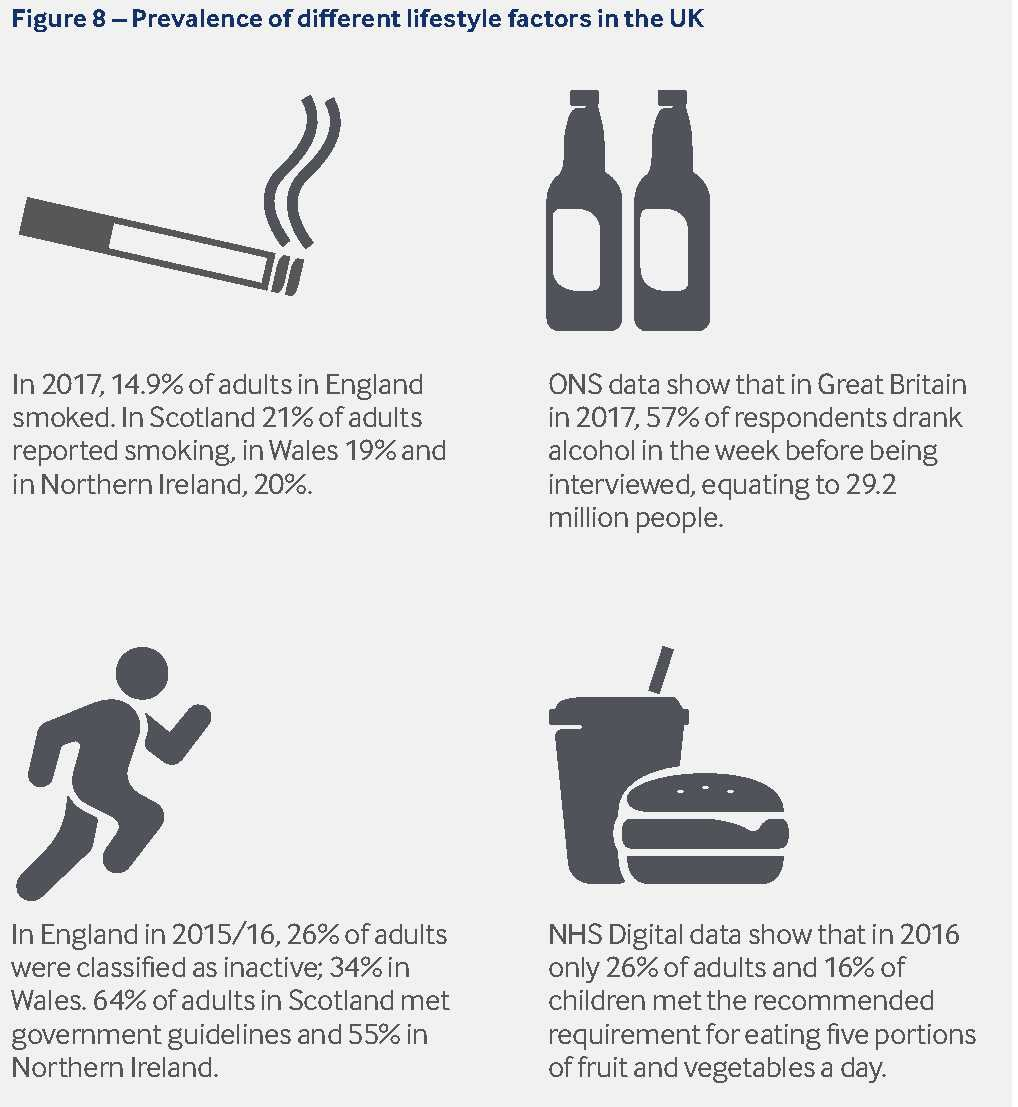
\includegraphics[width=3in]{images/ch3/15.png}
                    \caption{Prevalence of different lifestyle factors in the UK}
                \end{figure} 
            \begin{figure}[H]%option [H] means "strictly here"
                    \centering
                    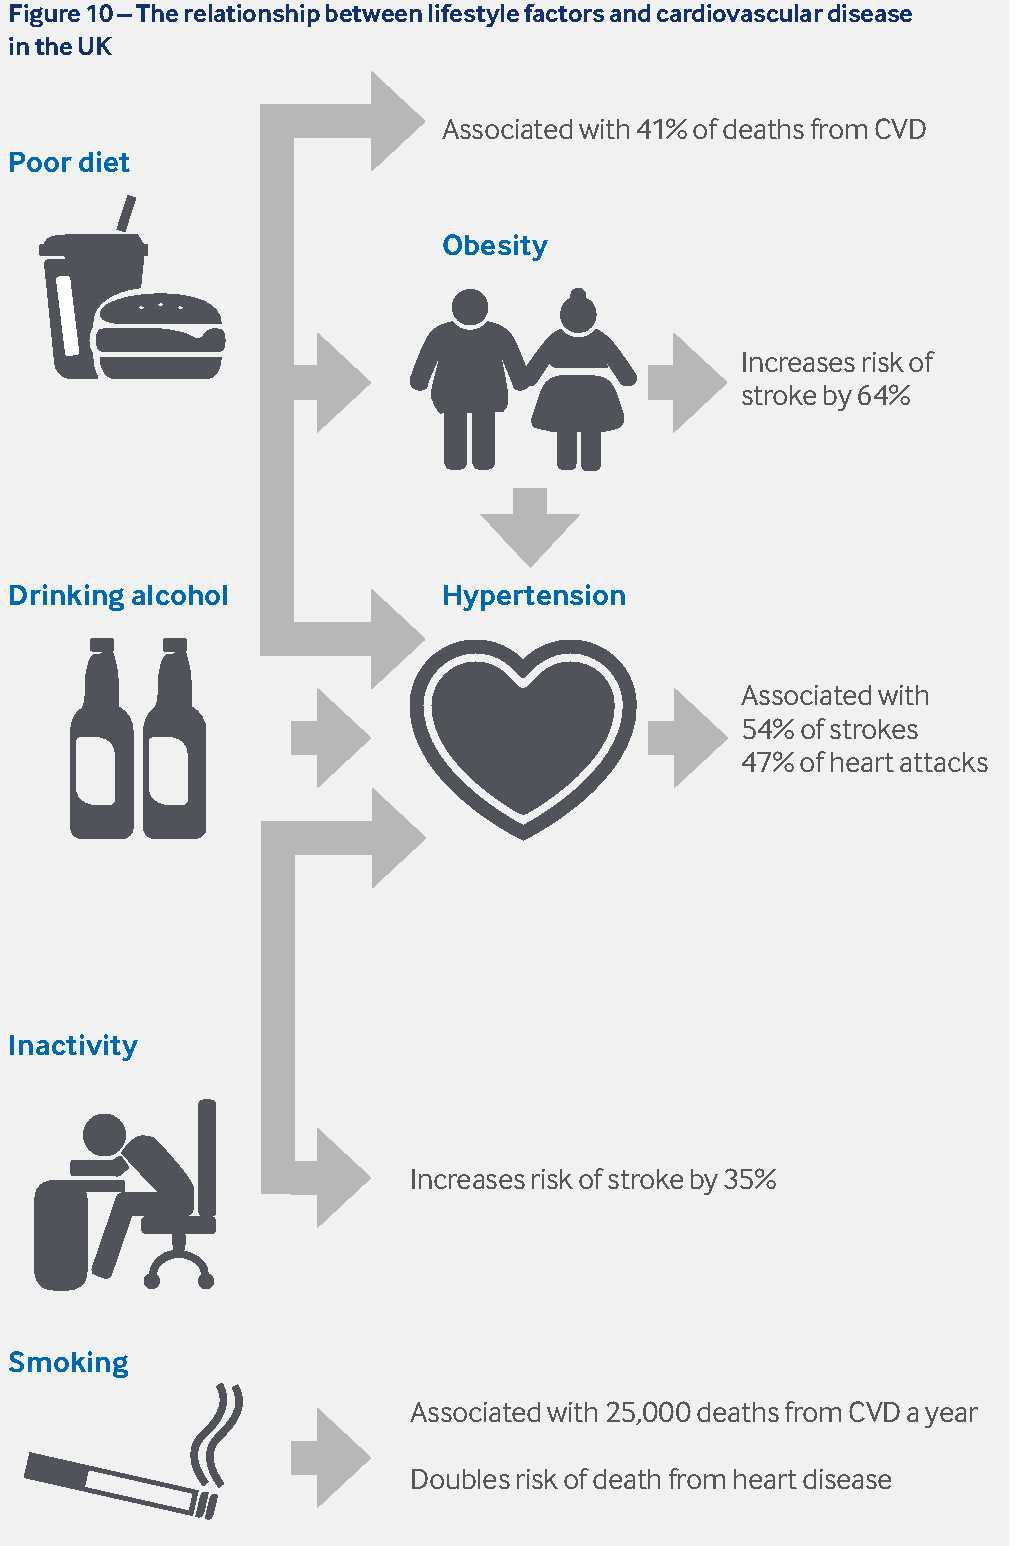
\includegraphics[width=3in]{images/ch3/16.png}
                    \caption{The relationship between different lifestyle factors and cardiovascular diseases in the UK}
                \end{figure} 

\begin{itemize}           
        \item Poor lifestyles, such as poor diet, drinking alcohol, inactivity and smoking, are associated with cardiovascular diseases.
        \end{itemize}

\begin{figure}[H]%option [H] means "strictly here"
                \centering
                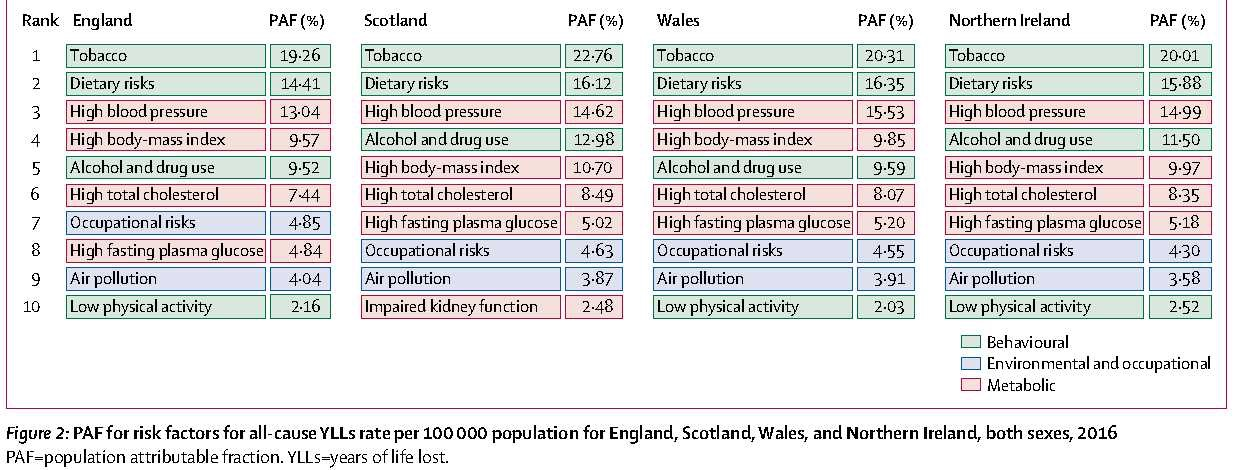
\includegraphics[width=5in]{images/ch3/17.png}
                \caption{PAF (Population Attributable Factions) for major risk factors for all-cause YLLs (Years of Life Lost) rate per 100,000 population for England, Scotland, Wales, and Northern Ireland, both sexes, 2016}
            \end{figure} 

\begin{itemize}           
        \item The population attributable fraction is the proportional reduction in population disease or mortality that would occur if exposure to a risk factor were reduced to an alternative ideal exposure scenario. 
        \item The ten leading risk factors contributing to YLLs were similar in rank across the four regions of the UK. Although the ranks were similar, the PAF of each risk factor varied in size in different countries, such as a higher PAF from tobacco in Scotland, and from alcohol and drug use in Scotland and Northern Ireland, compared with the other UK regions.
        \item Poor lifestyles do matter for health, although most money goes to curative health.
        \end{itemize}

        \subsection{How Is the Health Budget Spent?} 
        \subsubsection{Worldwide}
        
            \begin{figure}[H]%option [H] means "strictly here"
                \centering
                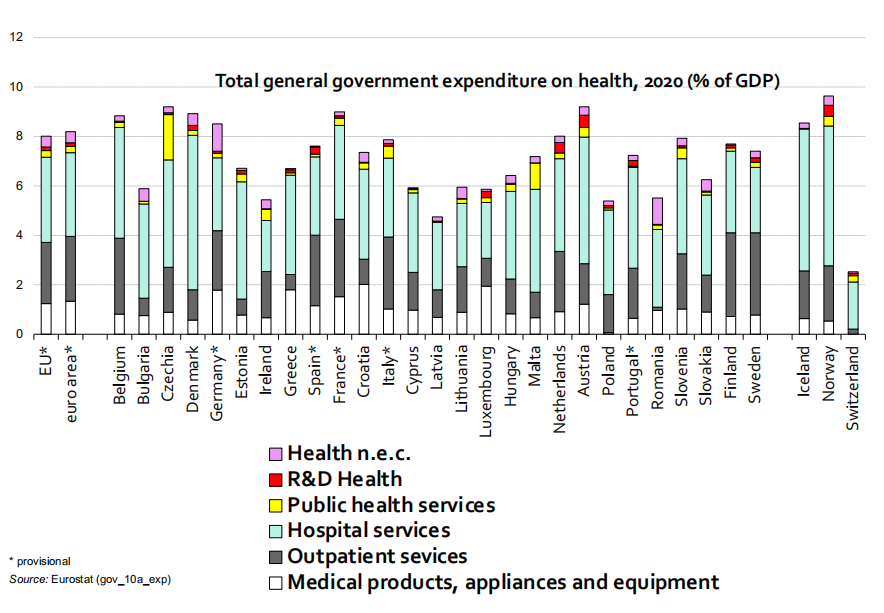
\includegraphics[width=4in]{images/ch3/10.png}
                \caption{Total general government expenditure on health as a percentage of GDP, 2020}
            \end{figure} 
        \begin{itemize}           
            \item The biggest share goes to hospital services, followed by outpatient services, so most money is used to treat people in the first place.
        \end{itemize}
        
        \subsubsection{UK}
        \begin{figure}[H]%option [H] means "strictly here"
                \centering
                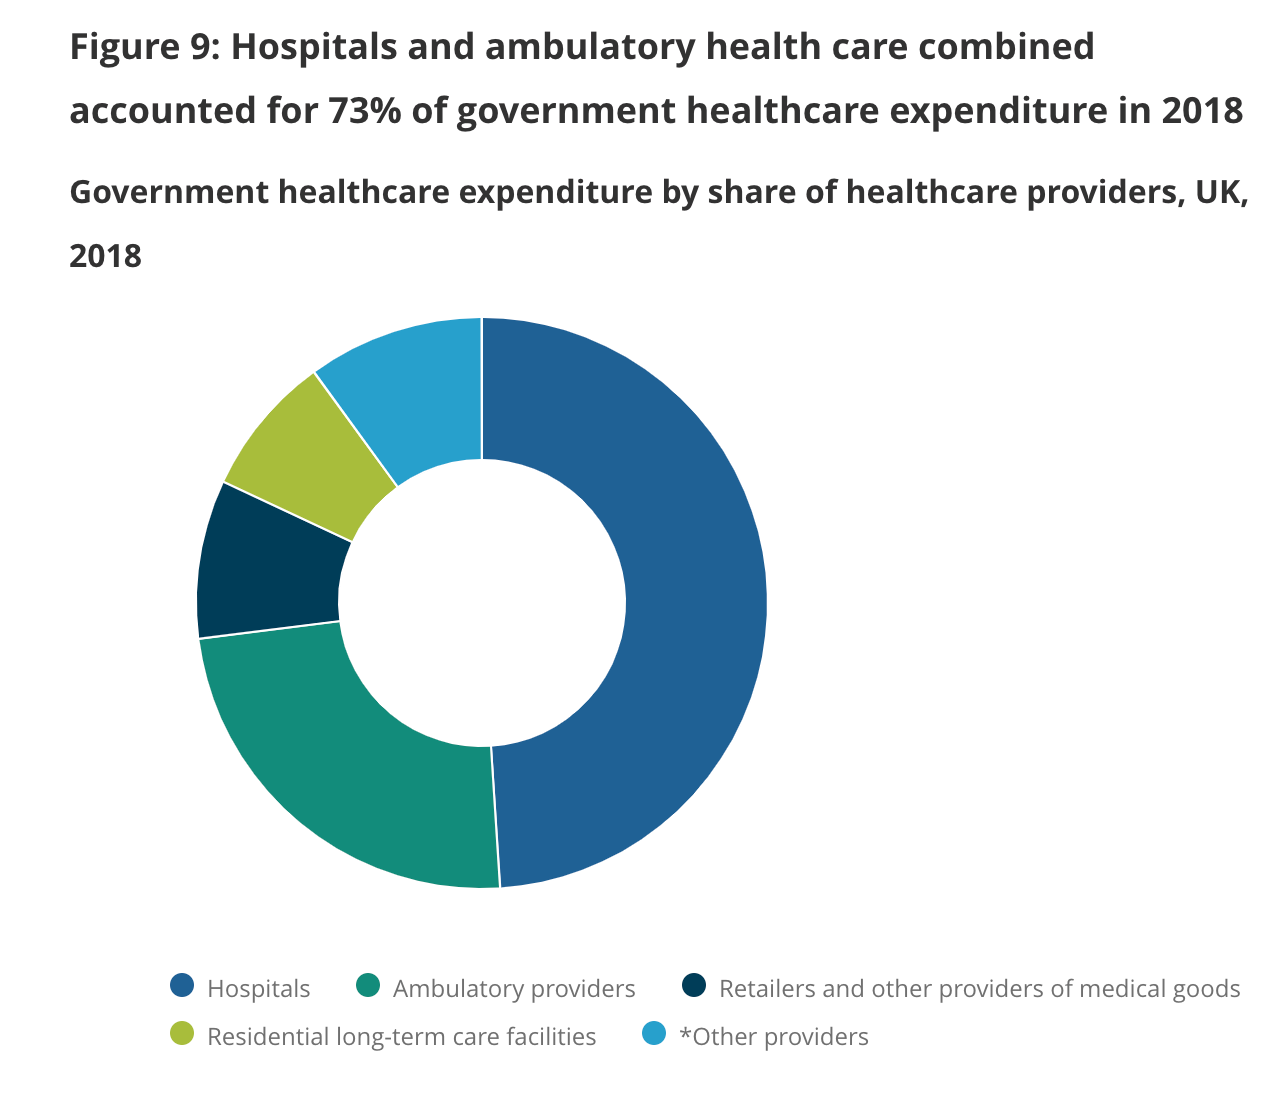
\includegraphics[width=4in]{images/ch3/18.png}
                \caption{Government healthcare expenditure by share of healthcare providers, UK, 2018}
            \end{figure} 
 \begin{itemize}           
        \item Hospitals and ambulatory healthcare combined accounted for 73 percent of government healthcare expenditure in 2018
        \end{itemize}              

\subsubsection{Preventive care expenditure is easy to cut, UK}
        \begin{figure}[H]%option [H] means "strictly here"
                \centering
                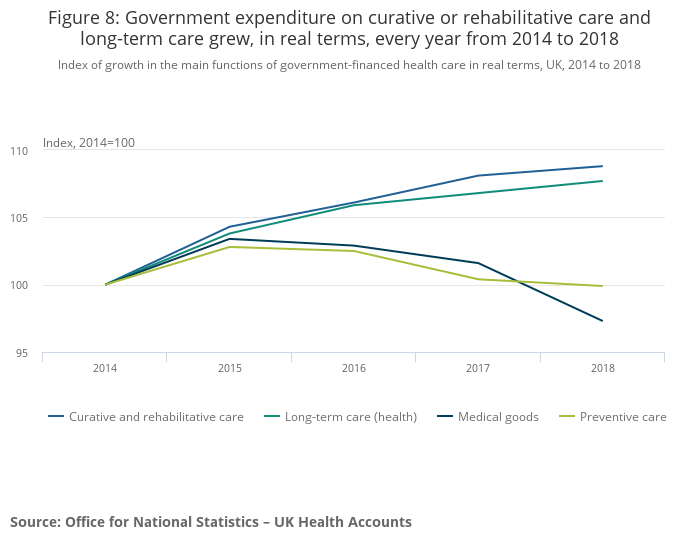
\includegraphics[width=4in]{images/ch3/19.png}
                \caption{Government expenditure on curative or rehabilitative care and long-term care grew, in real terms, every year from 2014 to 2018, index: 2014 = 100}
            \end{figure}
\begin{itemize}           
        \item Preventive care expenditure has decreased since 2015. This is because it is easy to cut. Curative care is difficult to cut, so the expenditure has increased over time.
        \end{itemize} 

        \begin{figure}[H]%option [H] means "strictly here"
                \centering
                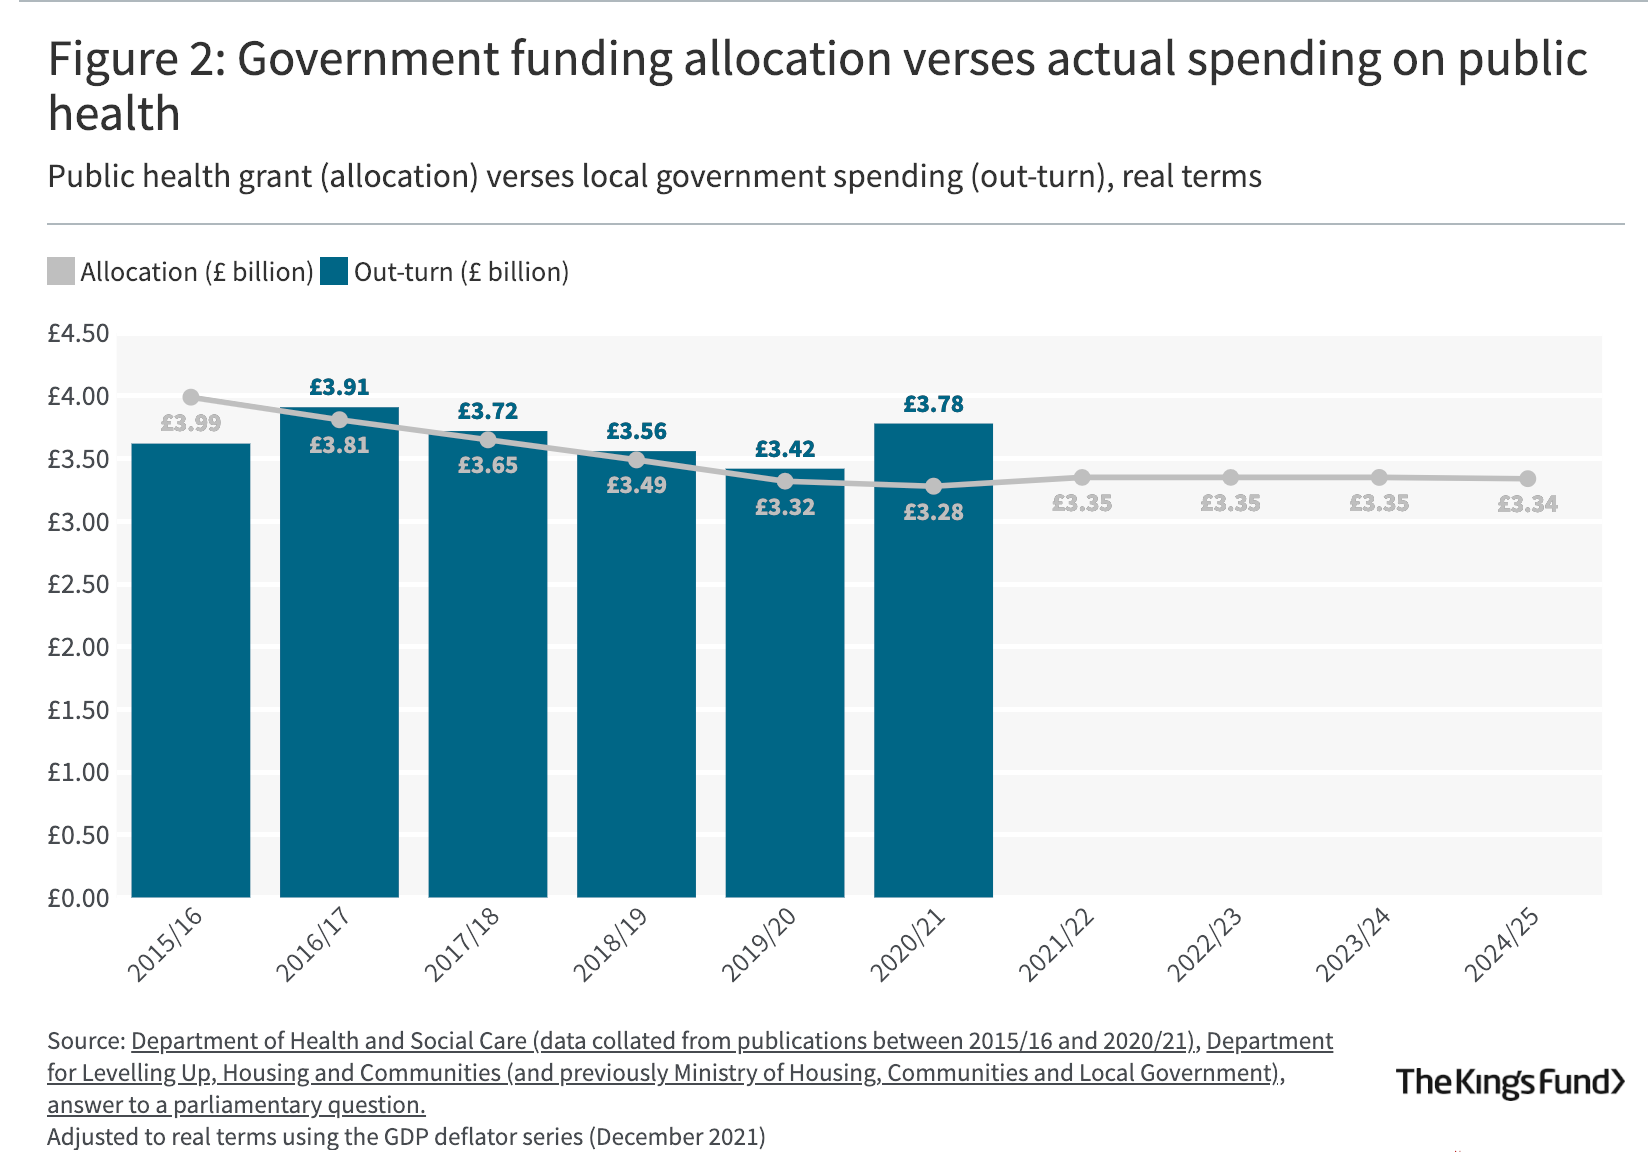
\includegraphics[width=4in]{images/ch3/20.png}
                \caption{Public health grant (allocation) VS local government spending (out-turn), real terms}
            \end{figure}
\begin{itemize}           
        \item The blue bars show the total local government spending on healthcare, which increased in 2020/21 due to Covid-19.
        \item The grey line shows the money allocated to public health prevention. It decreased since 2015/16. This is because it is easy to cut. 
        \end{itemize} 
        
        \begin{figure}[H]%option [H] means "strictly here"
                \centering
                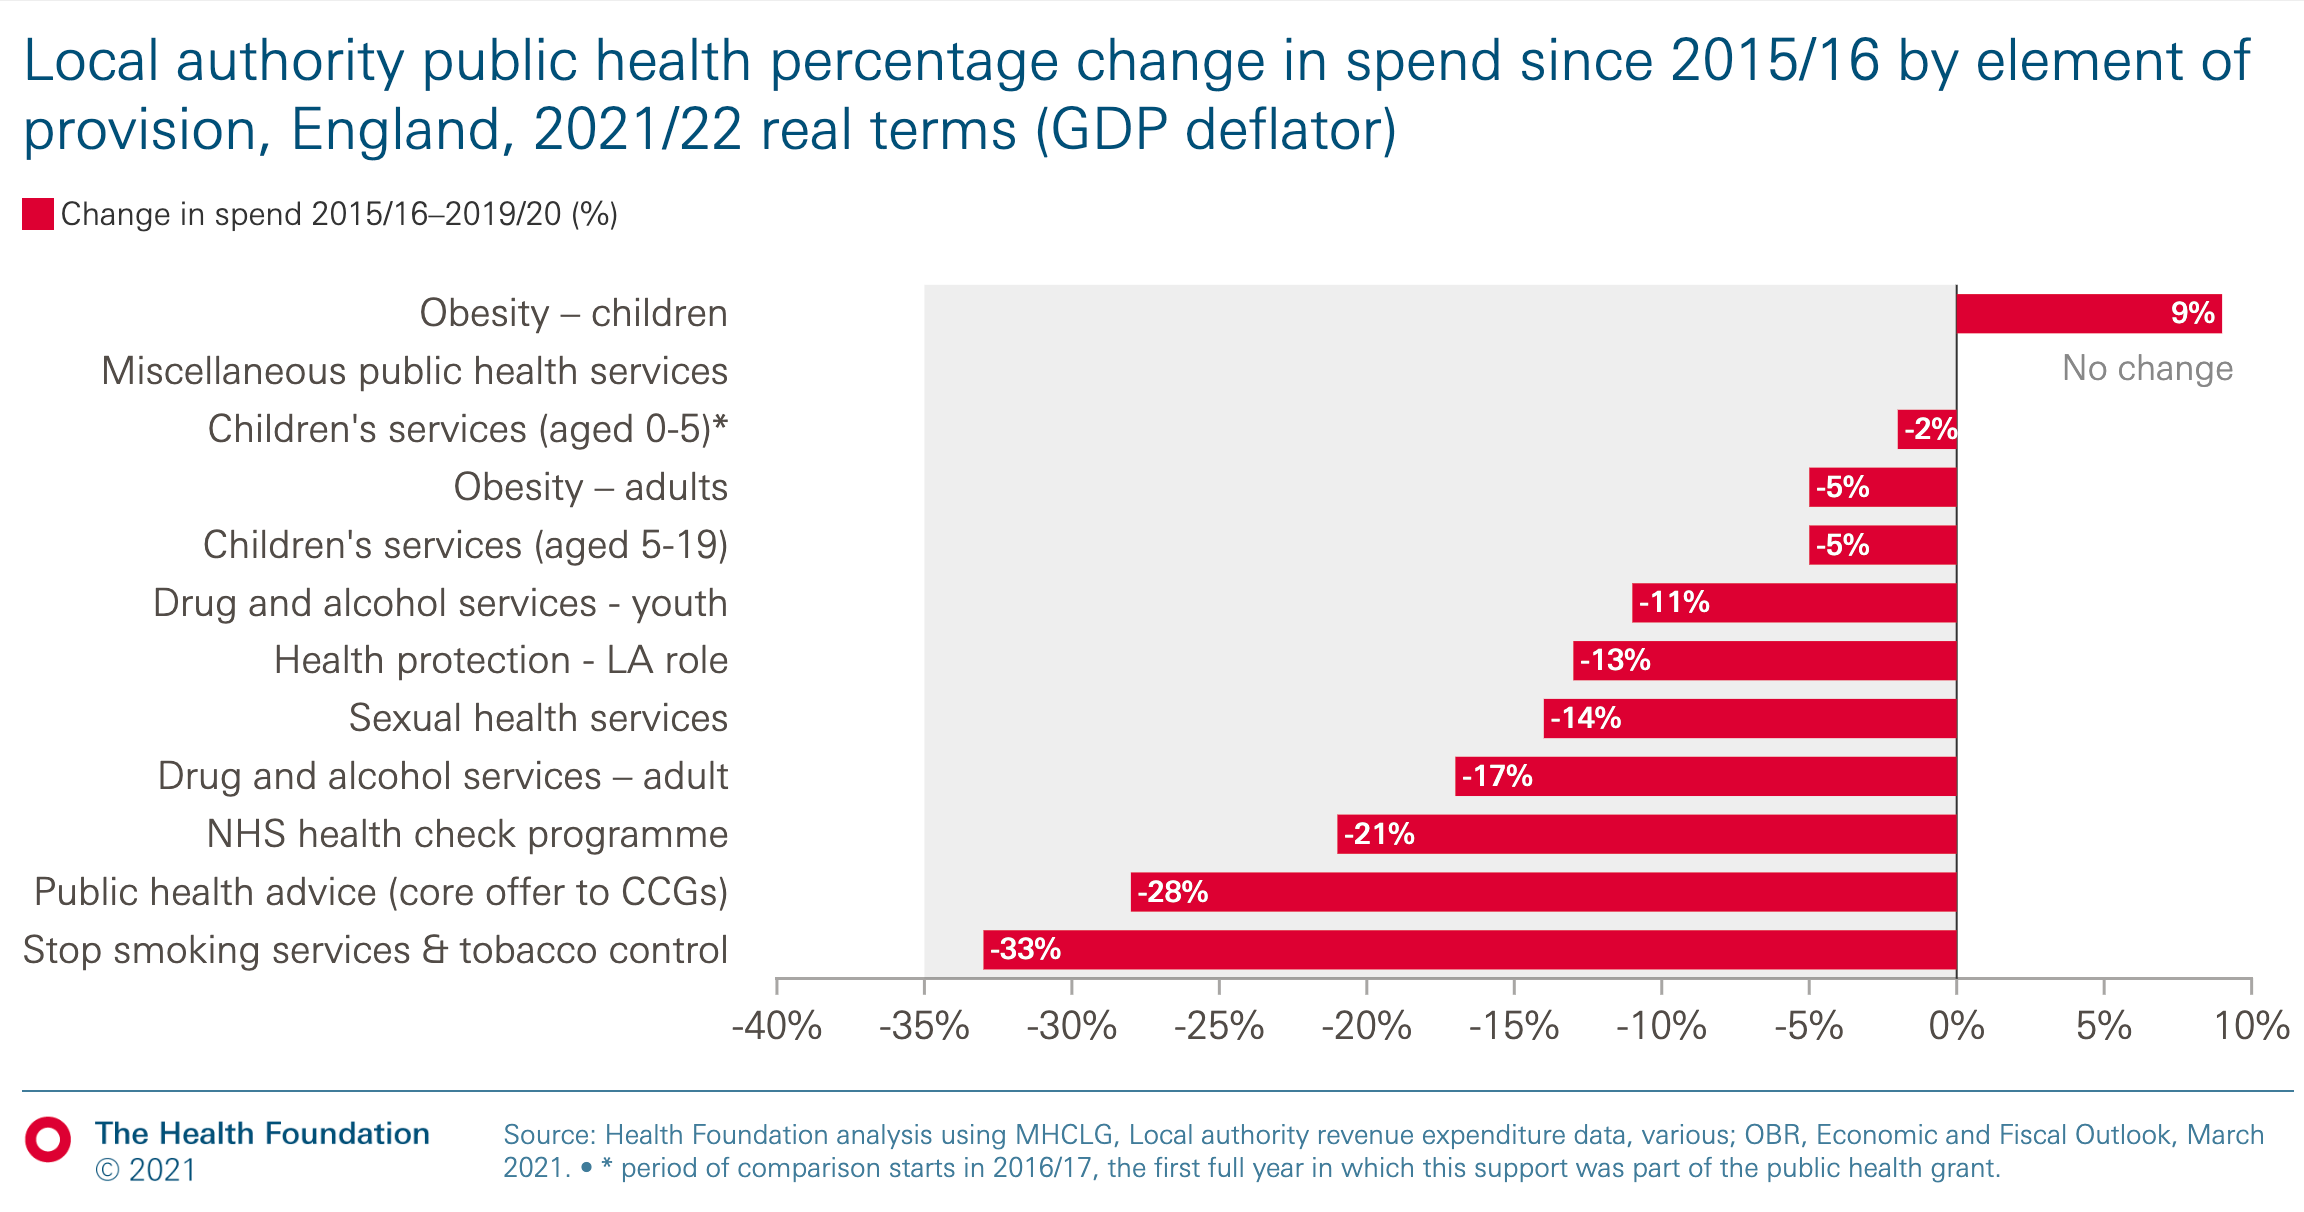
\includegraphics[width=4in]{images/ch3/21.png}
                \caption{Local authority public health percentage change in spending since 2015/16 by element of provision, England, 2021/22 real terms (GDP deflator)}
            \end{figure}
\begin{itemize}           
        \item For preventive healthcare expenditure, only obesity for children increased, since it is a major problem for children in the UK and costs NHS a lot of money. The expenditure is cut across all other categories.
        \end{itemize} 

        \subsection{Early Intervention and Prevention}
\begin{itemize}           
        \item Early intervention and prevention approaches aim to support health and wellbeing by taking action before health problems worsen, or by preventing health problems for occurring in the first place. 
        \item Public Health Prevention = improving public health through disease prevention
        a. Clinical interventions such as screening and vaccinations;
        b. Population-level measures aimed at influencing health behaviours or
addressing the social determinants of health (e.g. living conditions, education etc.).
        \item Early Intervention = strategies aimed to mitigate the effects of problems once they have been identified.
        – Some specifically targeted at the ‘early years’, including pregnancy, early parenting and the early parent-child relationship.
        \item A NICE (National Institute for Health and Care Excellence) review of the cost-effectiveness of 200 interventions found that 30 (15 percent) were cost-saving and 141 (70.5 percent) were cost-effective.
        \end{itemize} 

\subsection{Why government intervention in getting people to become healthier?}
        \begin{figure}[H]%option [H] means "strictly here"
                \centering
                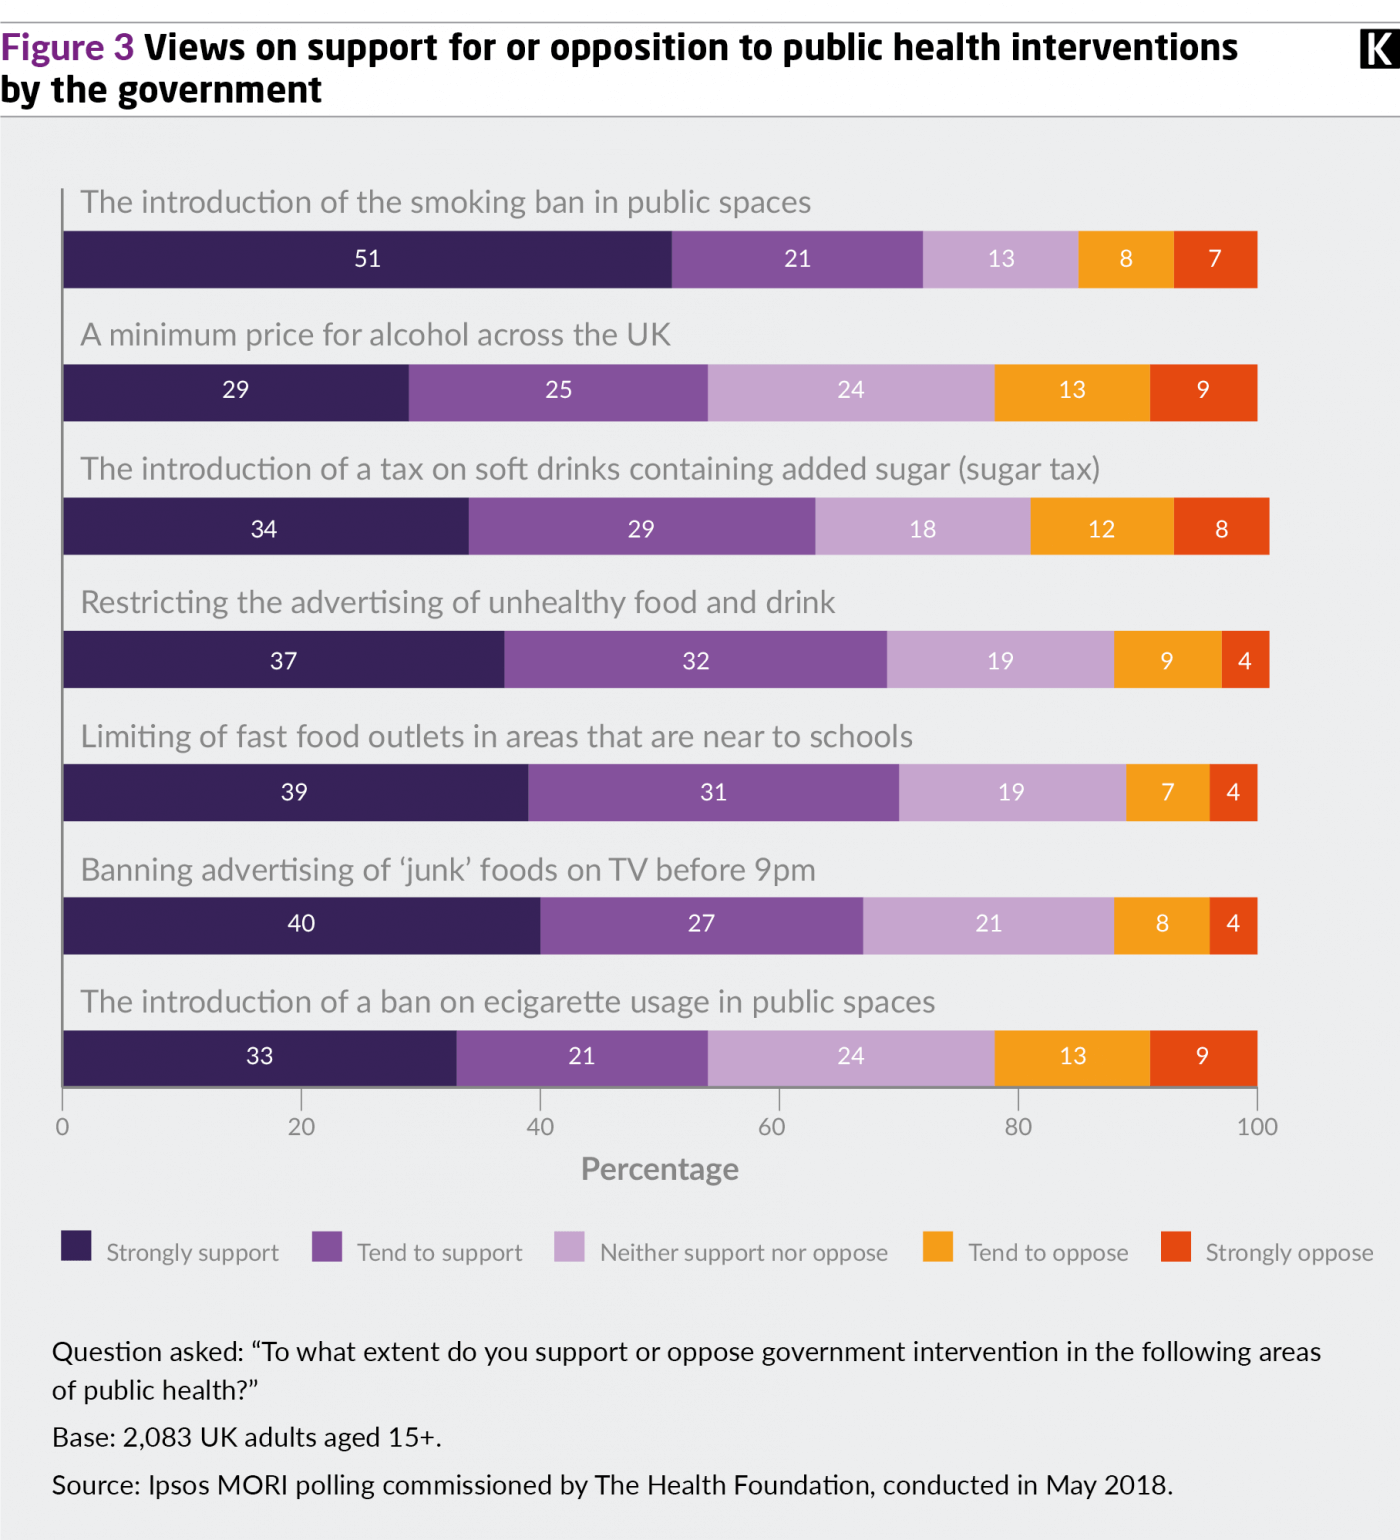
\includegraphics[width=4in]{images/ch3/22.png}
                \caption{Views on support for or opposition to public health interventions by the government}
            \end{figure}

\subsubsection{Reasons for government intervention:}          
\begin{itemize}           
        \item improve human capital, increase productivity, raise tax revenue in the future
        \item market failure: asymmetric information (e.g. junk food: consumers don't know the content/how much is going to harm them)
        \item public goods: hospital/public health services, nobody provides unless the government provides, it is expensive
        \item moral hazards
        \item negative externality (smoking)
        \item time-inconsistent preference (procrastination: go to the gym); addictive goods - the government can nudge/remind people
        \item In order to make progress and develop effective policies, we need first to understand how health is produced.
\end{itemize} 












\section{$\star$ The Production of Health as Human Capital: The Grossman Model}

    \subsection{Introduction}
    
        \begin{itemize}
            \item Grossman (1972) studied how individuals allocate their resources to produce health. He combined the theory of human capital and the theory of the allocation of time to explain the demand for health. Health is a unique good. We use time/resources/money to produce it and enjoy it.
            \item Four important aspects
            \begin{enumerate}
                    \item Health can be treated \emph{both as a consumption and an investment good}. As a \emphb{consumption good}, health yields direct utility. As an \emphb{investment good}, health increases the number of healthy days available to participate in the market and non-market activities.
                    \item Health lasts for more than one period. It \emphb{depreciates} (e.g. ageing process; if no vaccine immunity, poorer health; if don't go to the gym, poorer health) and can be analyzed like a capital good.
                    \item Individuals are not passive consumers of health: they produce it, spending time and money (buy market inputs).
                    \item Demand for medical care is derived: people demand medical care not per se, but to produce health.
                \end{enumerate}
            \item As both a consumption and an investment good, optimal health capital accumulation requires the decision-making of its owner – the individual – who is \emph{both the consumer and the producer}.    
        \end{itemize}        

    \subsection{Preferences, Utility, and Death}
    
        Health as a consumption good enters directly into utility. Here, we model an individual's \emphb{Intertemporal Utility Function} as:
        \begin{equation*}
            U = U(\underbrace{\varphi_0 H_0}_{h_0},...,\underbrace{\varphi_n H_n}_{h_n},Z_0,...,Z_n)
        \end{equation*}
        where:
        \begin{itemize}
            \item $H_0$ : inherited stock of health (predetermined)
            \item $H_i$ : stock of health in the $i$th time period
            \item $\varphi_i$ : service flow per unit stock
            \item $h_i$ = $\varphi_iH_i$ : healthy days
            \item $Z_i$ : non-health commodity
        \end{itemize}
        Length of life is \emph{endogenous}: \emphb{death} occurs when $H = H_{min}$. The lifespan is determined by individuals' choices of working time ($TW_i$), time spent on producing health investment ($TH_i$), time spent on producing non-health commodities ($T_i$), and the purchase of other market inputs ($M_i$).
        
        Individuals \emph{maximise their utilities} subject to resource (time/budget) constraints (section \ref{sec:health_res_cons}) and production technologies (section \ref{sec:health_tech_cons}) introduced below.

    \subsection{Two Resource Constraints}\label{sec:health_res_cons}
    
        Here, we have 2 constraints: the budget constraint and the time constraint.

        The \emphb{Budget Constraint} is:
        \begin{equation*}
            \sum_{i=0}^n\frac{P_iM_i+V_iX_i}{(1+r)^i}=\sum_{i=0}^n\frac{W_i \times TW_i}{(1+r)^i}+ A_0
        \end{equation*}
        \begin{equation*}
            \text{PV of Health and Non-Health Commodities} = \text{PV of Labour Earnings} + \text{Initial Assets}
        \end{equation*}
        where:
        \begin{itemize}
            \item $P_i$ : price for health
            \item $V_i$ : price for non-health commodity
            \item $M_i$ : good inputs in the production of health
            \item $X_i$ : good inputs in the non-health commodity
            \item $W_i$ : wage rate
            \item $TW_i$ : time spent working 
            \item $A_0$ : initial assets
            \item $r$ : interest rate
        \end{itemize}
        The \emphb{Time Constraint} is:
        \begin{equation*}
            \underbrace{TW_i+TH_i+T_i}_{h_i} +TL_i= \aleph
        \end{equation*}
        where:
        \begin{itemize}
            \item $TW_i$ : time spent on working
            \item $TH_i$ : time spent on producing health
            \item $T_i$ : time spent on producing other goods we enjoy
            \item $TL_i$ : time loss due to illness
            \item  $\aleph$  : overall time endowment ($\aleph = h_i + TL_i$)
            \item $h_i$ : healthy days ($h_i=TW_i+TH_i+T_i$)
        \end{itemize}    
    
    \subsection{Production Technologies (Production Constraints)}\label{sec:health_tech_cons}
    
        Here, we have 5 production functions in total:

        The \emphb{Healthy Time Production Function} is:
        \begin{equation*}
            h_i=f(H_i)
        \end{equation*}
        which means healthy days can be produced by some technology using health stocks.
        
        The \emphb{Health Stock Production Function} is:
        \begin{equation*}
            H_{i+1}=H_i-\delta_i H_i+I_i
        \end{equation*}
        where:
        \begin{itemize}
            \item $I_i$ : gross investment
            \item $\delta_i$ : depreciation (exogenous, might vary with age, e.g. older, higher depreciation)
        \end{itemize}
        The health stock PF implies that when investment is high, an individual can overcome the high rate of depreciation.

        Such specification brings \emph{two problems}:
        \begin{itemize}
            \item Linearity: It does not account for diminishing marginal returns
            \item It does not account for random shocks
        \end{itemize}

        The \emphb{2 Household Production Functions} are:

        Production of health investment ($I_i$):
        \begin{equation*}
            I_i=I_i(M_i,TH_i;E_i)
        \end{equation*}
        Production of non-health commodities ($Z_i$):
        \begin{equation*}
            Z_i=Z_i(X_i,T_i;E_i)
        \end{equation*}
        where
        \begin{itemize}
            \item $M_i$ = good inputs in the production of health
            \item $X_i$ = good inputs in the production of non-health commodity
            \item $TH_i$ : time spent on producing health
            \item $T_i$ : time spent on producing other goods we enjoy
            \item $E_i$ : stock of human capital (education) $\implies$ better education, better health
        \end{itemize}
        We can see that the production of health and non-health commodities needs both time and money. (Cooking and going to the gym also matter.) 

        The \emphb{Income Production Function} is:
        \begin{equation*}
            Y_i = W_i\times TW_i
        \end{equation*}
           
    \subsection{The Production Possibility Frontier}

        The \emphb{Production Possibility Frontier} shows the frontier of the feasible set of non-health commodities ($Z$) health stock ($H$).

        Since an individual dies and cannot consume/produce any non-health commodities, we must have $Z_i=0$ when $H_i \leq H_{min}$.

        This is a WRONG example:
        \begin{figure}[H]
            \centering
            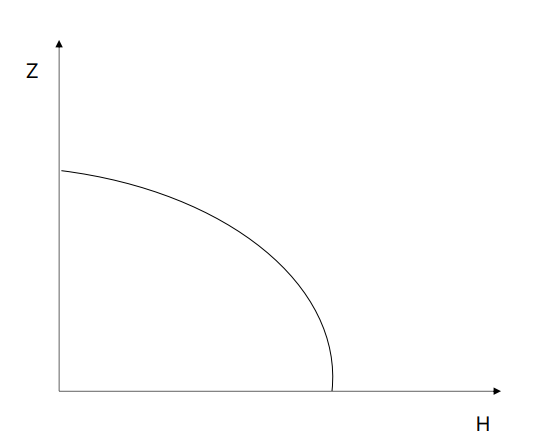
\includegraphics[width=3in]{images/ch3/23.png}
            \caption{Wrong PPF}
        \end{figure}
        A CORRECT example and \emphb{Optimality}:
        \begin{figure}[H]
            \centering
            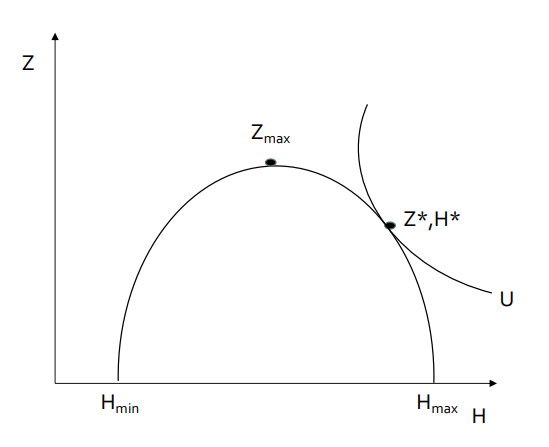
\includegraphics[width=3in]{images/ch3/24.png}
            \caption{Correct PPF and the Optimal Point}
        \end{figure}
        We must have $H_{min}$, $Z_{max}$, and $H_{max}$.  We reach the optimal point ($Z^*,H^*$) when the indifference curve is tangent to the PPF. In the following 2 sections, we will explain this is also level of health stock where MEC and COC curves intersect.

    \subsection{MEC and COC Curves}

        The \emphb{Marginal Efficiency of Health Capital (MEC)} curve shows the value of the additional healthy days gained from a 1-unit increase in the health stock (MPH). MEC is the monetary value of the marginal productivity of health stocks. It is diminishing as an individual's health stock expands.

        MEC has the following expression:
        $$MEC=MPH\times w$$
        where:
        \begin{itemize}
            \item $w$: wage rate
            \item $MPH$: marginal productivity of health stock
        \end{itemize}

        The \emphb{Cost of Capital (COC)} curve represents the supply price of capital or the cost of holding an additional unit. Its position is determined by the depreciation rate of the health stock ($\delta$) and the opportunity cost of holding health capital (r):
        $$COC=r+\delta$$

    \subsection{Optimisation, Demand for Health, and Ageing}

        \subsubsection{Optimisationa and Demand for Health}\label{grossman_demand}
    
            \emphb{Optimality Conditions} for the simplest version of the model:
            \begin{equation*}
                \color{red} \text{PV of the Marginal Cost of Gross Health Investment} = \text{PV of Marginal Benefits of Health}
            \end{equation*}
            We have seen this is the tangent point of the FPF and indifference curve. Meanwhile, this is also the point where the Marginal Efficiency of Health Capital (MEC) curve intersects the Cost of Capita (COC) curve:
            \begin{equation*}
                \color{red} \underbrace{r+\delta}_{MC\ (COC)} = \underbrace{MPH \times w}_{MB\ (MEC)}
            \end{equation*}
            \begin{figure}[H]
                \centering
                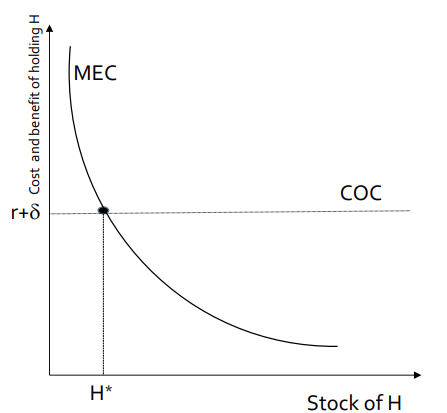
\includegraphics[width=3in]{images/ch3/25.png}
                \caption{MEC and COC of Holding Health Stocks and the Optimal Point}
            \end{figure}

        \subsubsection{What Happens as We Age?}
            \begin{figure}[H]
                \centering
                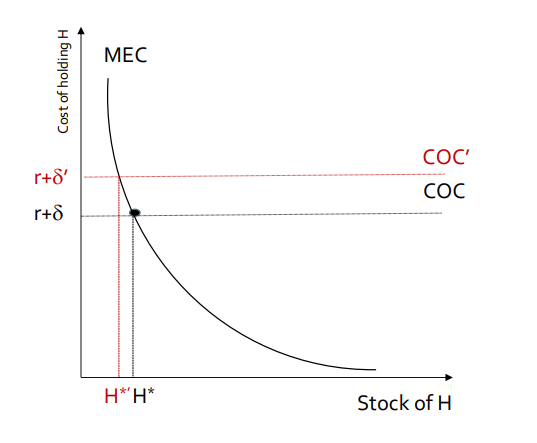
\includegraphics[width=3.5in]{images/ch3/26.png}
                \caption{Optimality and Aging}
            \end{figure}
            The depreciation rate increases ($\delta \to \delta'$) as we age, so the COC shifts upwards to COC', and the optimal level of health stock we can sustain is lower ($H^* \to H*'$).

        \subsubsection{Health Inequality}

            See section \ref{health_ineq_cause}.

    \subsection{Literature Development and Criticisms}
    
        Since 1972, the Grossman model has been the cornerstone for modelling investment in health capital, spurring a great deal of research, extensions, empirical testing and criticism. Grossman himself reviewed the literature many times, e.g. in the 2000 Chapter “The Human Capital Model” in the Handbook of Health Economics.
        
        Some of the main \emphb{criticisms} of the Grossman model:
            \begin{itemize}
                \item It does not preclude an individual choosing to live forever (Ehrlich and Chuma, JPE 1990 “does not determine the length of life")
                \item It does not provide an adequate conceptual framework for the SES (socioeconomic status)-health gradient (Galama and van Kippersluis, EJ, 2018): They develop a model which incorporates health, longevity, wealth, earnings, education, work, job-related physical and psychosocial health stressors, leisure, health investment (e.g. exercise, medical care) and healthy and unhealthy consumption (including housing, neighbourhood social environment).
                \item Not faithful to gerontological models of health deficit accumulation (Strulik).
                \item It does not include an early childhood phase (Heckman, PNAS 2007).
            \end{itemize}
            
        It is a very active area of research, both theoretically and empirically.




\section{Inequalities in Health}\

    Inequalities in health are not random and are associated with characteristics. Poor people are less healthy, maybe because they eat cheaper food and don't know the benefit of doing exercise (less educated). Education is correlated with health.

    More educated  $\to$  Higher income  $\to$  More resources and information

    \subsection{SES Inequalities in BMI Widen over the Lifecycle and across British Cohorts}
    
        \begin{figure}[H]%option [H] means "strictly here"
            \centering
            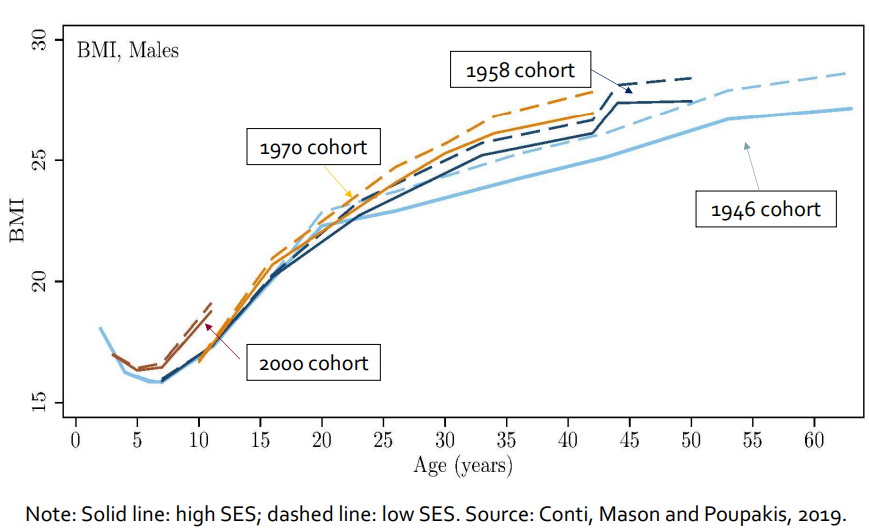
\includegraphics[width=4in]{images/ch3/27.png}
            \caption{SES Inequalities in BMI Widen over the Lifecycle and across British Cohorts}
        \end{figure}
        \emphb{BMI (Body Mass Index)} is not the best measure of body fitness, since it only includes two dimensions (weight and height), it doesn't take into account fat mass, it doesn't include many diseases such as blindness, it is developed in the West and thus the norms may not apply to other ethnicities. However, BMI is a relatively \emph{simple measure}, and it is correlated with obesity and worse body conditions later in life.
        \begin{itemize}
            \subsubsection{Lifecycle:}
            \item The lines are very close in the beginning, the 1946 cohort starts to diverge at the end of adolescence and keeps diverging as they get older. 
            \item Low SES people have higher BMIs than high SES people as they get older.
            \item For each cohort, BMI generally increases as age increases. 
            \subsubsection{Cohort:}
            \item 2000 cohort has a higher BMI at the young age.
            \item The health inequality (divergence) presents in every cohort, and we are not doing anything to effectively reduce it.
        \end{itemize}       
        
    \subsection{Health inequalities are everywhere}
    
        \begin{itemize}
            \item Researchers have documented inequalities in the distribution of health by socioeconomic status, gender, and ethnicity.
            \item Research on socio-economic inequalities in health in the UK has a long history, together with nice data.
            \item In the early part of the 20th century the British government introduced questions on occupation in the decennial census:
            \item The 1970-1972 Decennial Supplement of occupational Mortality (OCPS) showed that men in social class V (unskilled) were 2.5 times as likely to die before the age of 65 than those in social class I (professional). Children in social class V families were twice as likely to die as those in social class I.
        \end{itemize} 

    \subsection{Landmark Studies in Social Class Inequalities in Health in the UK}

        \subsubsection{Brief Listing}
            \begin{itemize}
                \item \emphb{Black Report (1980)}
                \begin{itemize}
                    \item Health inequalities were widening, the problem had little to do with NHS.
                    \item Four possible explanations: (1) data artefact; (2) social selection (sicker people $\Rightarrow$ less able to study and work $\Rightarrow$ poorer); (3) behaviour; (4) material circumstances.
                    \item Policy recommendation: reduce poverty, spend more on prevention.
                \end{itemize} 
                
                \item \emphb{Whitehead Report (1987)}
                \begin{itemize}
                    \item Commissioned by the Health Education Council (HEC) and headed by
        Margaret Whitehead.
                    \item Health inequalities widened since the Black Report.
                    \item HEC was scrapped: was campaigning on alcohol, tobacco and diet issues which upset some of the government’s financial supporters.
                \end{itemize}
                
                \item \emphb{Acheson Report (1998)}
                \begin{itemize}
                    \item Commissioned by the new Labour (Blair) government in 1997, under the chairmanship of a former Chief Medical Officer, Sir Donald Acheson.
                    \item Similar findings and recommendations as the Black Report: the root cause of inequalities in health was poverty.
                \end{itemize}
        
                \item \emphb{Whitehall I Study}
                \begin{itemize}
                    \item Examined over 18,000 male British civil servants over 10 years, starting in 1967.
                    \item Showed that mortality was higher among those in the lower grade than in the higher grade – for all causes and CHD.
                    \item Controlling for risk factors (smoking, obesity, exercise, blood pressure) accounted for 40 percent of the gradient.
                \end{itemize}
        
                \item \emphb{Whitehall II Study}
                \begin{itemize}
                    \item Examined 10,308 civil servants aged 35-55, 2/3 men and 1/3 women, starting in 1985.
                    \item Showed social gradient for several diseases.
                    \item Added job-related stress to the traditional risk factors for low social class.
                \end{itemize}
        
                \item \emphb{Fair Society, Healthy Lives: The Marmot Report (2010)}
                \begin{itemize}
                    \item Concluded that reducing health inequalities would require action on six policy objectives: number 1 is “Give every child the best start in life”.
                \end{itemize}
        
                \item \emphb{Health Equity in England: The Marmot Review 10 Years On (2020)}
                \begin{itemize}
                    \item “This ‘10 years on’ report shows that, in England, health is getting worse for people living in more deprived districts and regions, health inequalities are increasing  and, for the population as a whole, health is declining. The data that this report brings together also show that for almost of all the recommendations made in the original Marmot Review, the country has been moving in the wrong direction. In particular, lives for people towards the bottom of the social hierarchy have been made more difficult. Some of these difficulties have been the direct result of government policies, some have resulted from failure to counter adverse trends such as increased economic inequalities or market failures.”
                \end{itemize}
            \end{itemize} 

        \subsubsection{The Marmot Review}
            \begin{figure}[H]
                \centering
                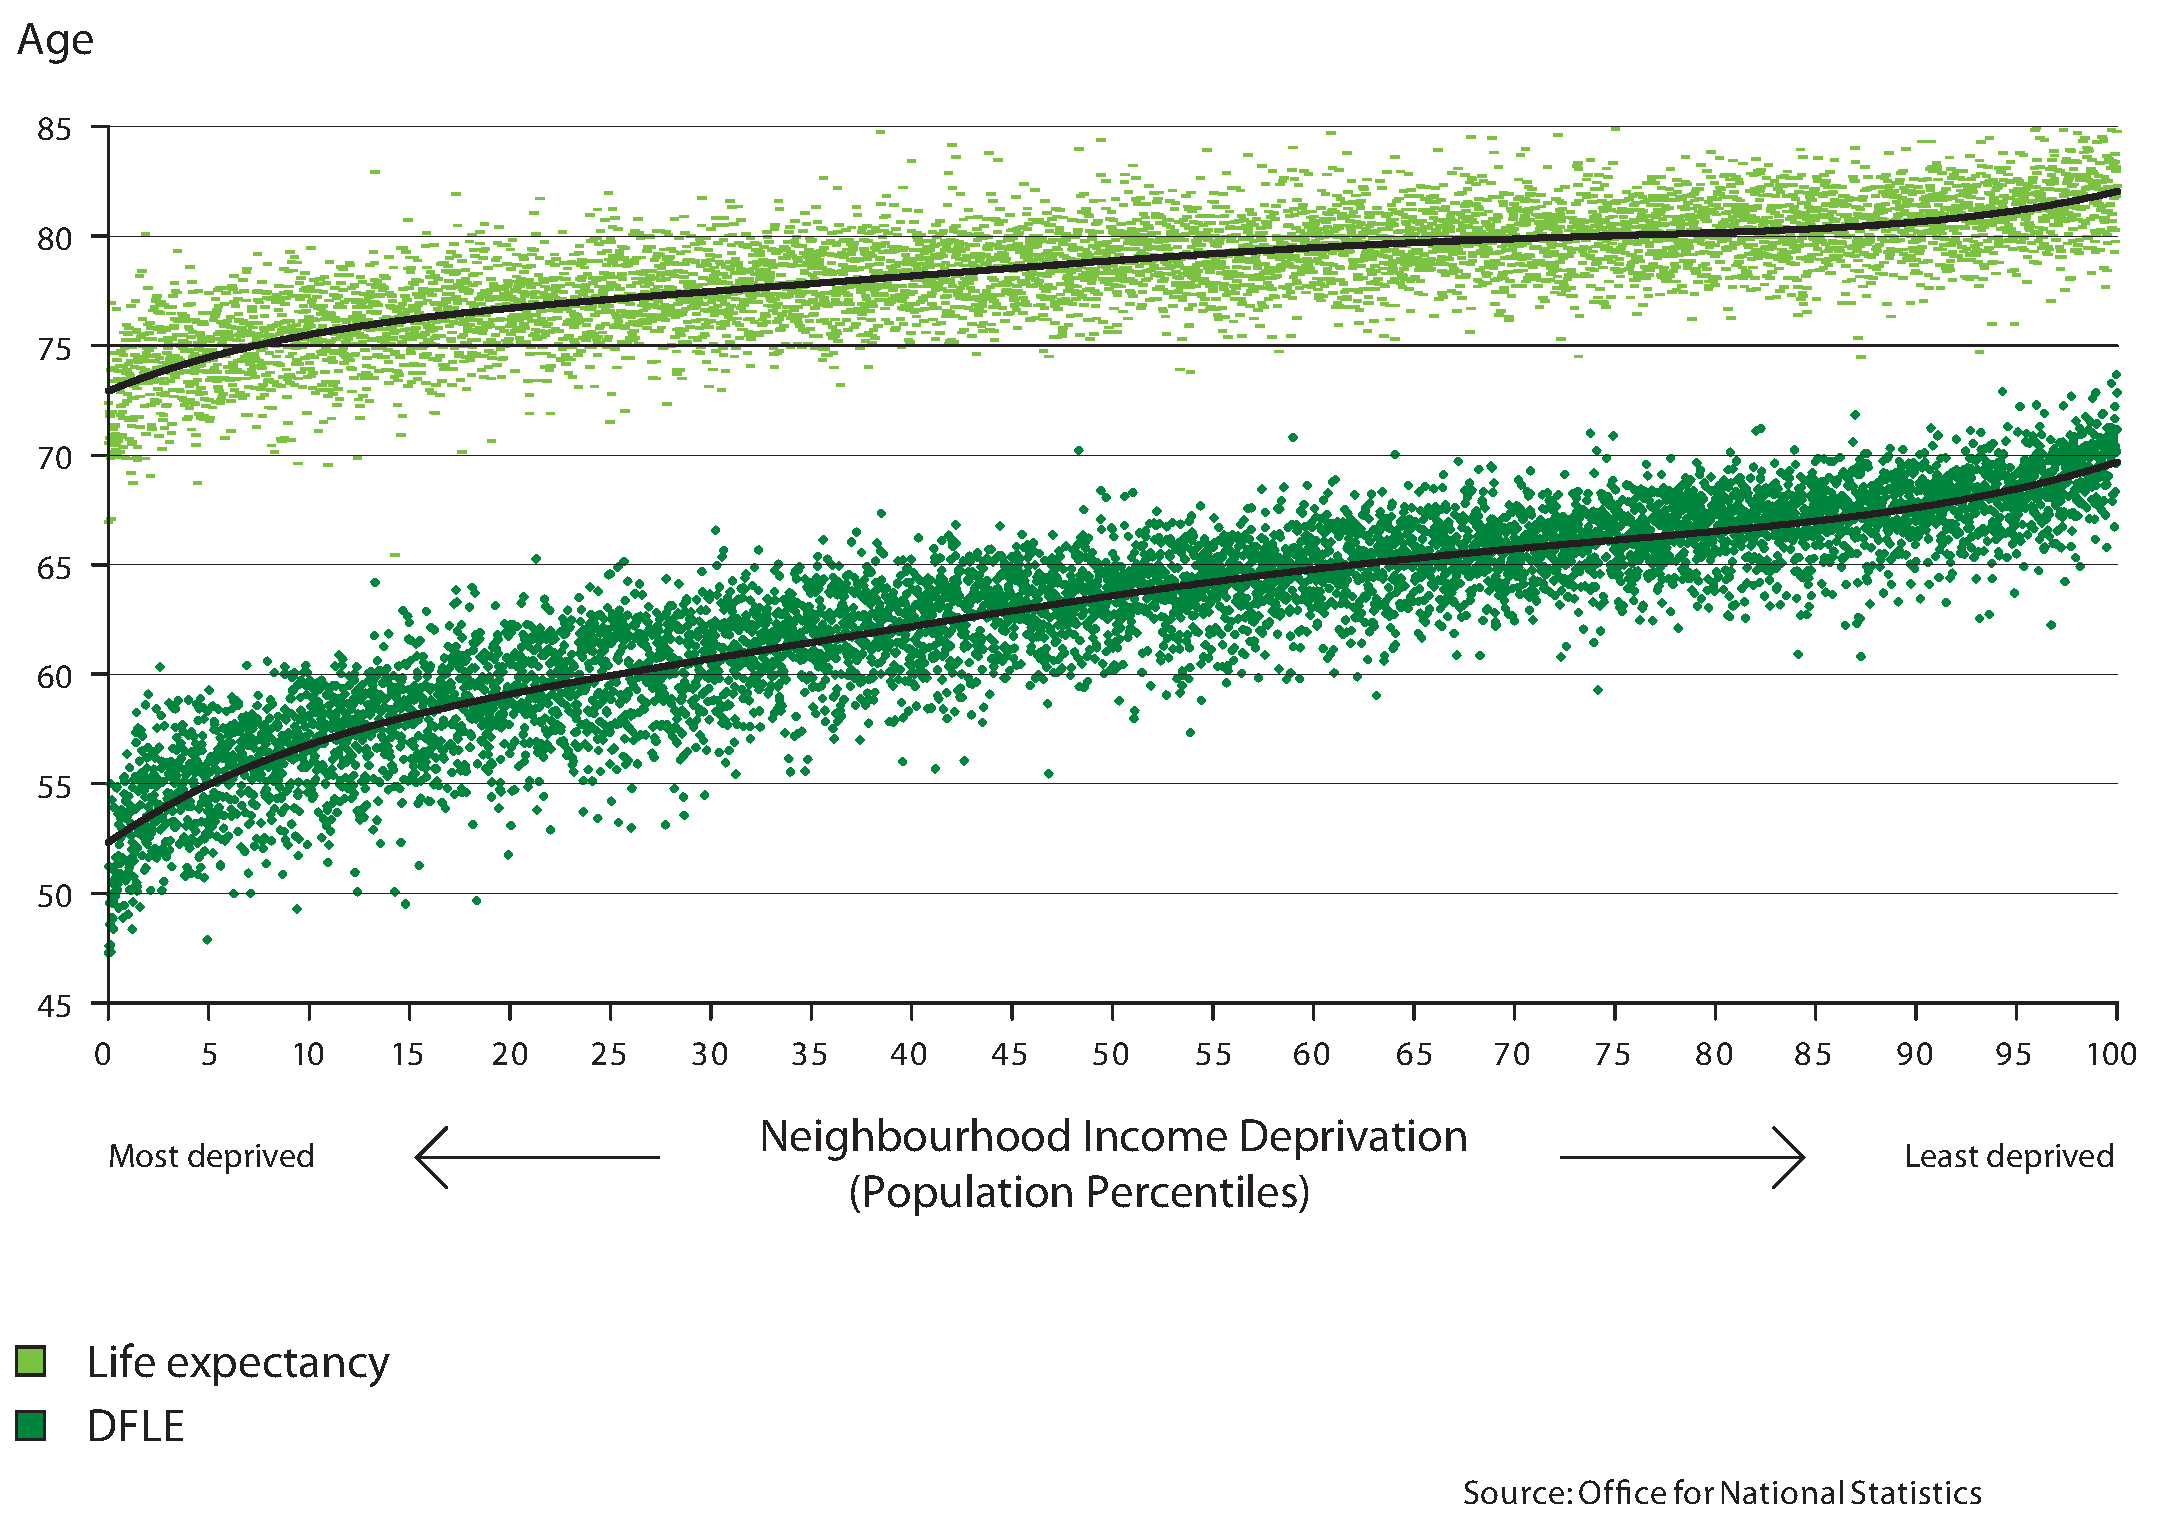
\includegraphics[width=4in]{images/ch3/28.png}
                \caption{Life expectancy and disability-free life expectancy (DFLE) at birth, by neighbourhood income level, England, 1999-2003}
            \end{figure}
            \begin{itemize}
                    \item \emphb{Disability-Free Life Expectancy (DFLE)} measures not only how long you live but also how well you live, so there is a gap between life expectancy and DFLE.
                    \item There is a discrepancy in the life expectancy/DFLE between the most deprived and the least deprived people in England.
            \end{itemize} 
        
            \begin{figure}[H]
                \centering
                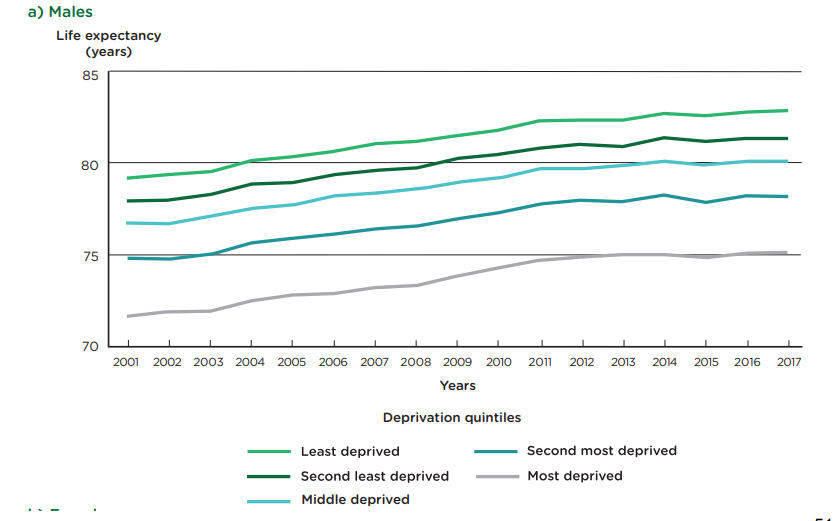
\includegraphics[width=4in]{images/ch3/29.png}
                \caption{Life expectancy at birth by area deprivation quintiles and sex, England, 2003–05 to 2015–17}
            \end{figure}
            \begin{itemize}
                \item Life expectancy is increased for everyone.
                \item The most deprived has the lowest life expectancy.
                \item The gaps between groups are almost the same as time passed, so inequalities stay the same.
            \end{itemize}
        
        \subsubsection{Public Health England}
            \begin{figure}[H]
                \centering
                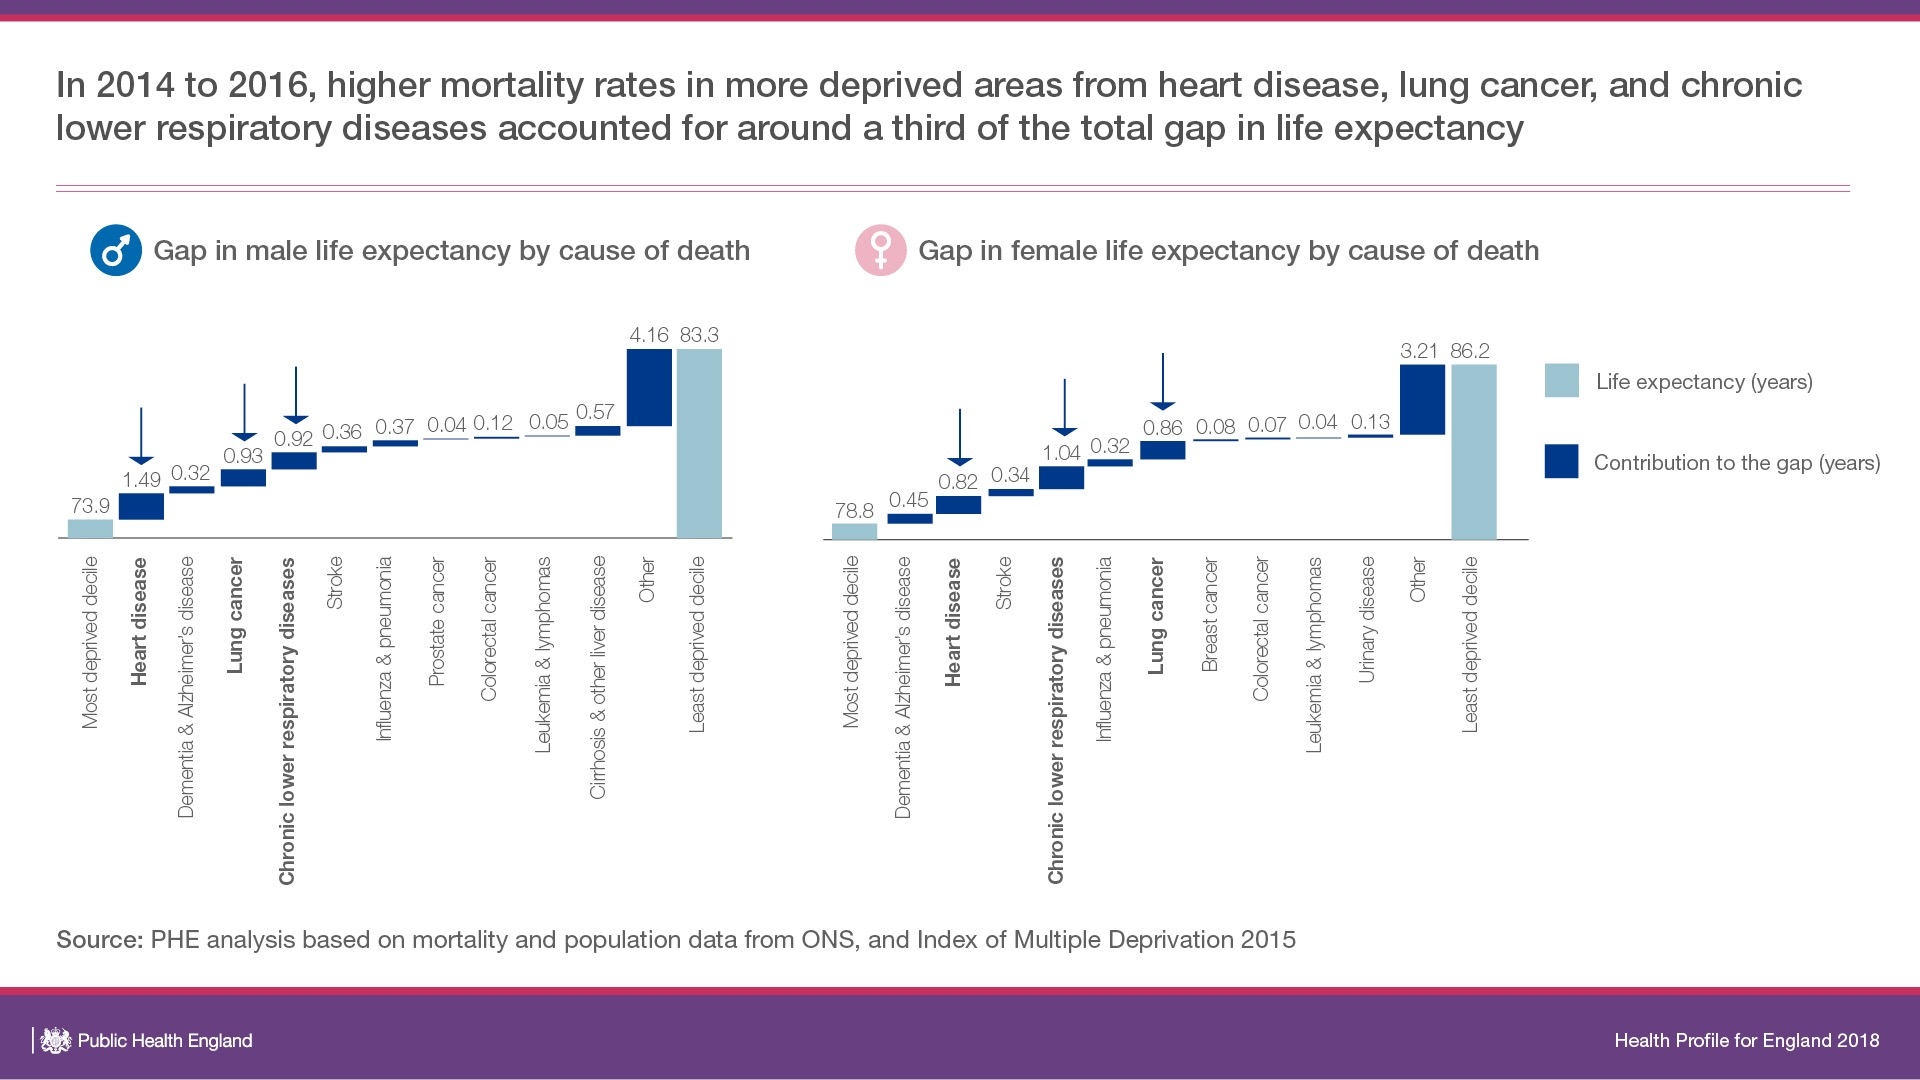
\includegraphics[width=5in]{images/ch3/30.png}
                \caption{What causes of death are driving the gap in life expectancy among the most deprived people and the least deprived people, male/female}
            \end{figure}
          In 2014 to 2016, higher mortality rates in more deprived areas from heart disease, lung cancer, and chronic lower respiratory diseases accounted for around a third of the total gap in life expectancy.
        
        \subsubsection{The IFS Deaton Review (2019-)}
            \begin{figure}[H]
                \centering
                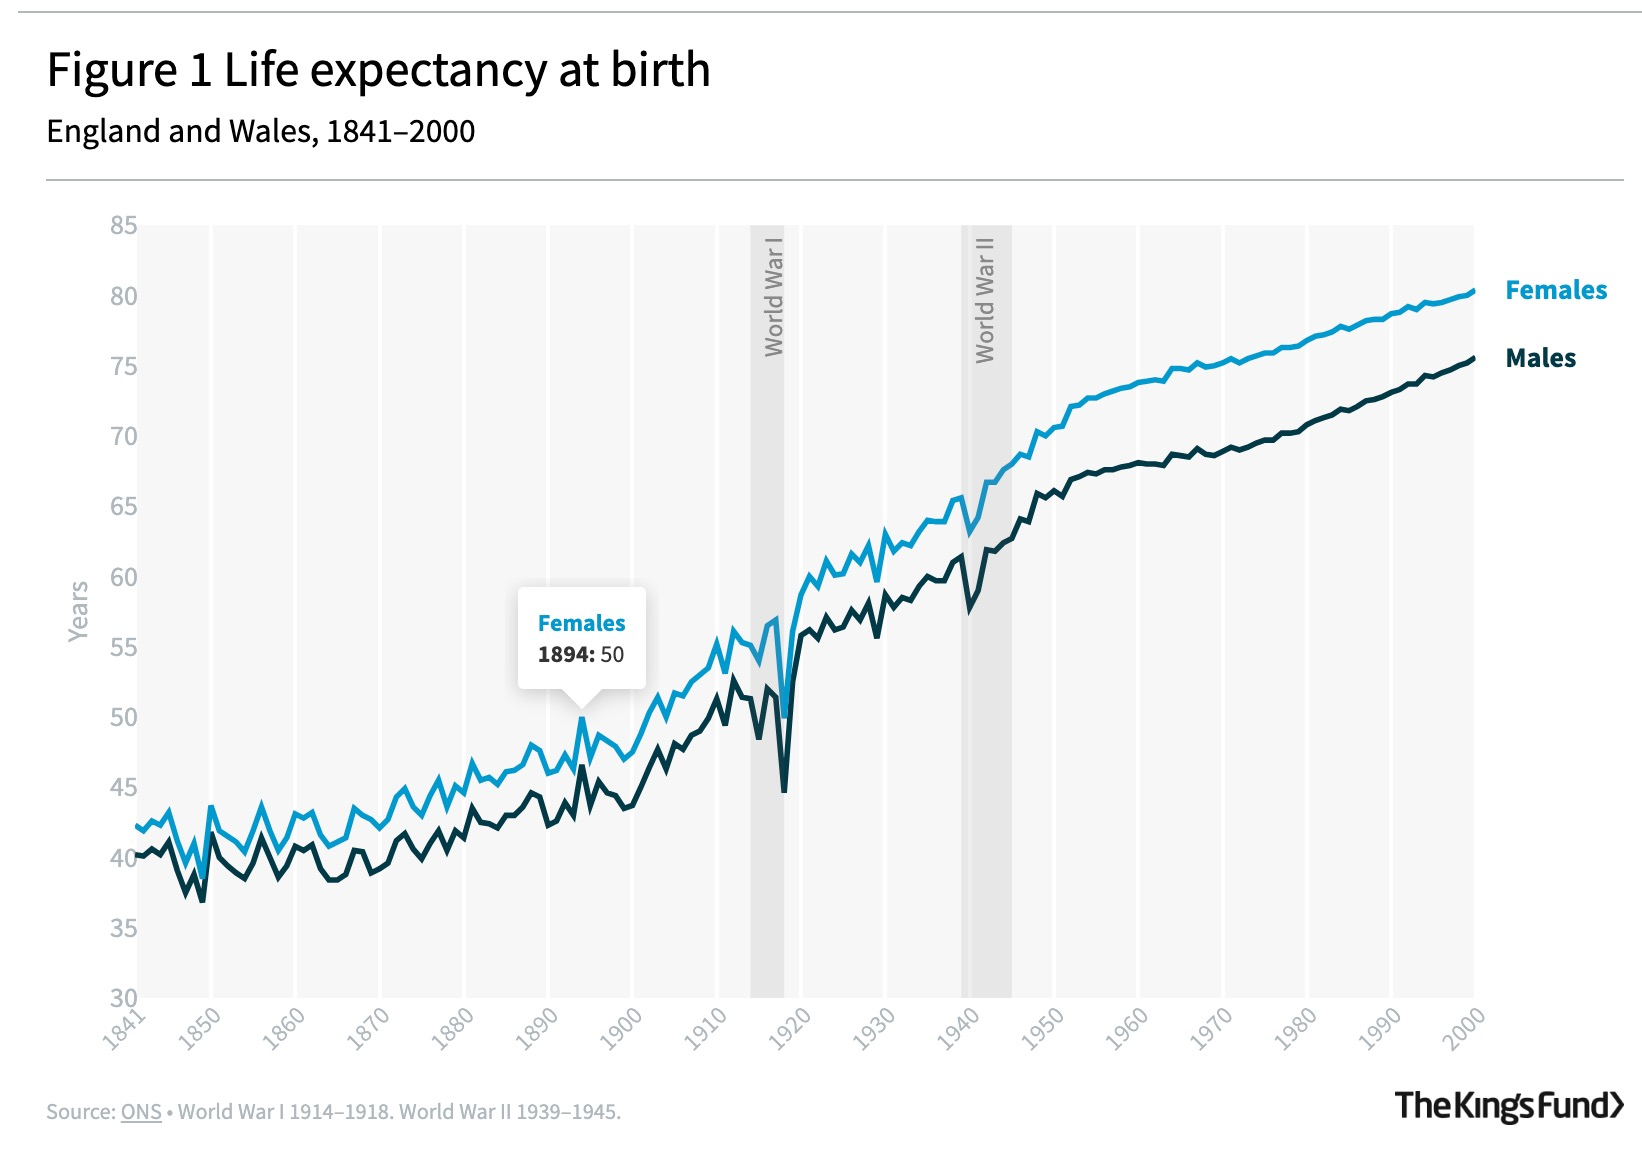
\includegraphics[width=4in]{images/ch3/31.png}
                \caption{Life expectancy at birth, England and Wales, 1841-2000, Males/Females}
            \end{figure}
            The life expectancy increased and almost doubled. Females had higher life expectancy. The biggest drop was in World War II.
         
            \begin{figure}[H]
                \centering
                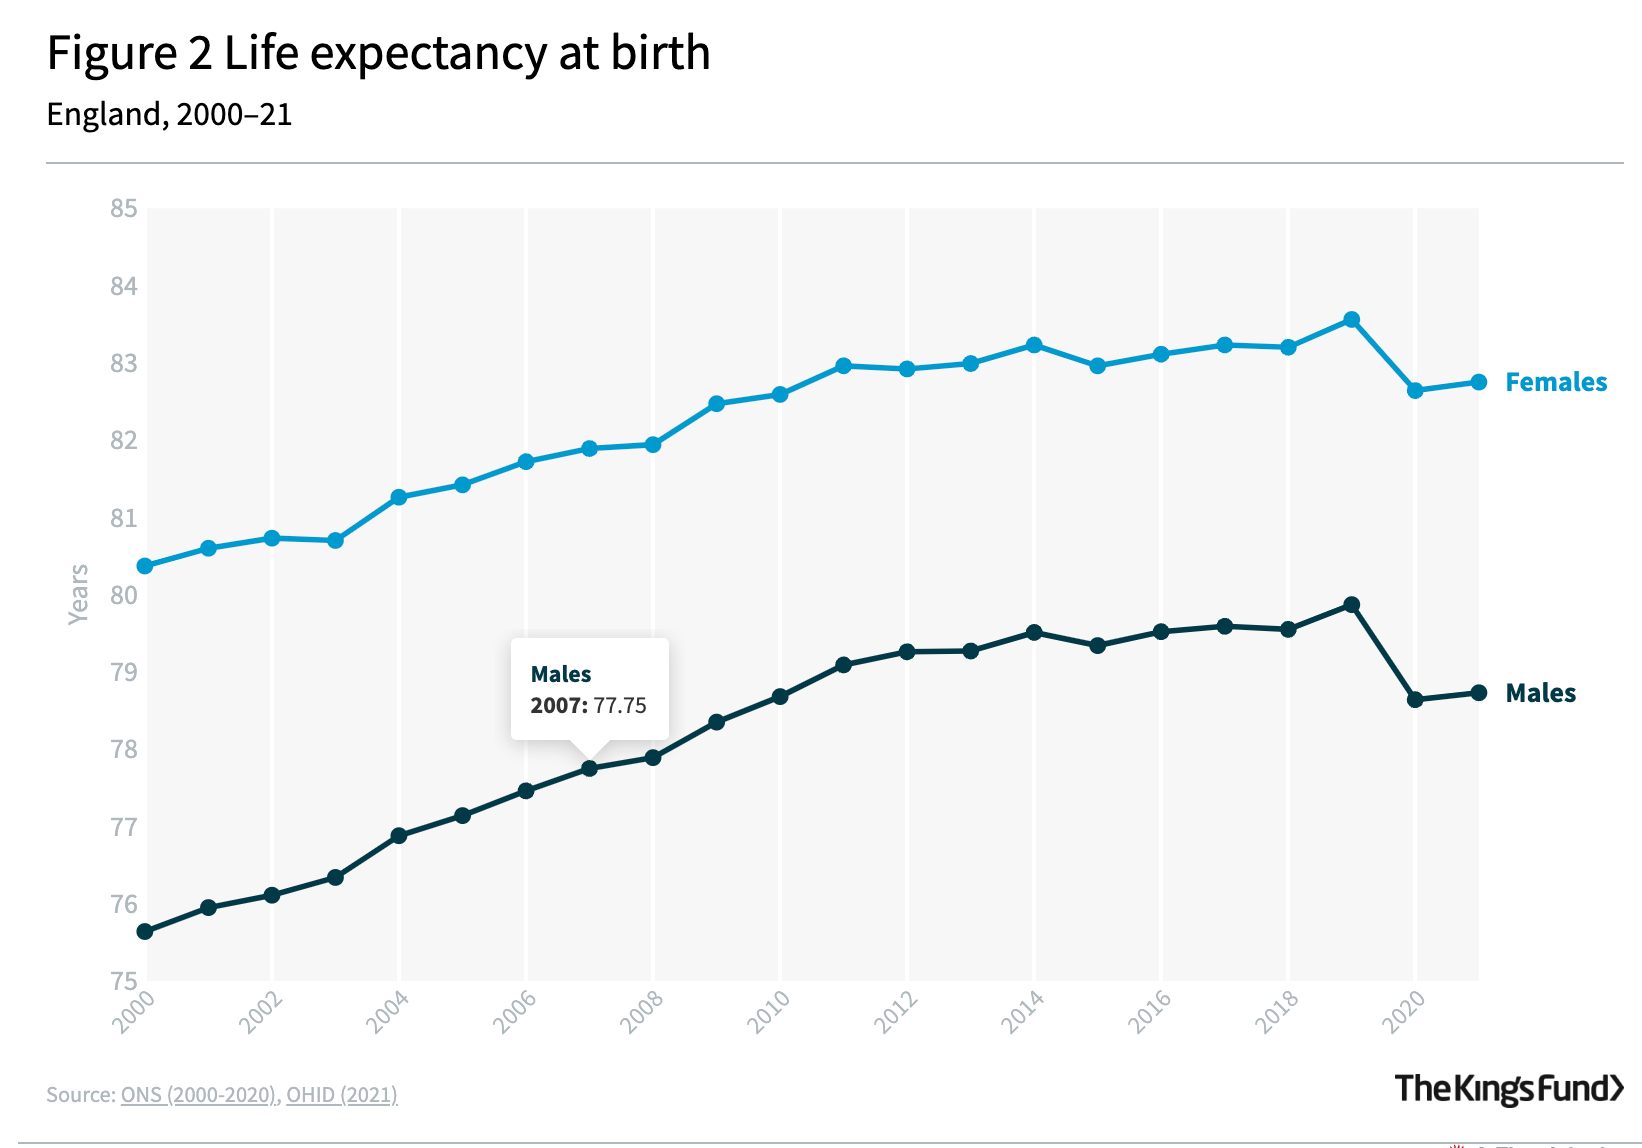
\includegraphics[width=4in]{images/ch3/32.png}
                \caption{Life expectancy at birth, England, 2000-2021, Males/Females}
            \end{figure}        
            The second biggest drop was during the pandemic (about 1 year). 
        
            \begin{figure}[H]
                \centering
                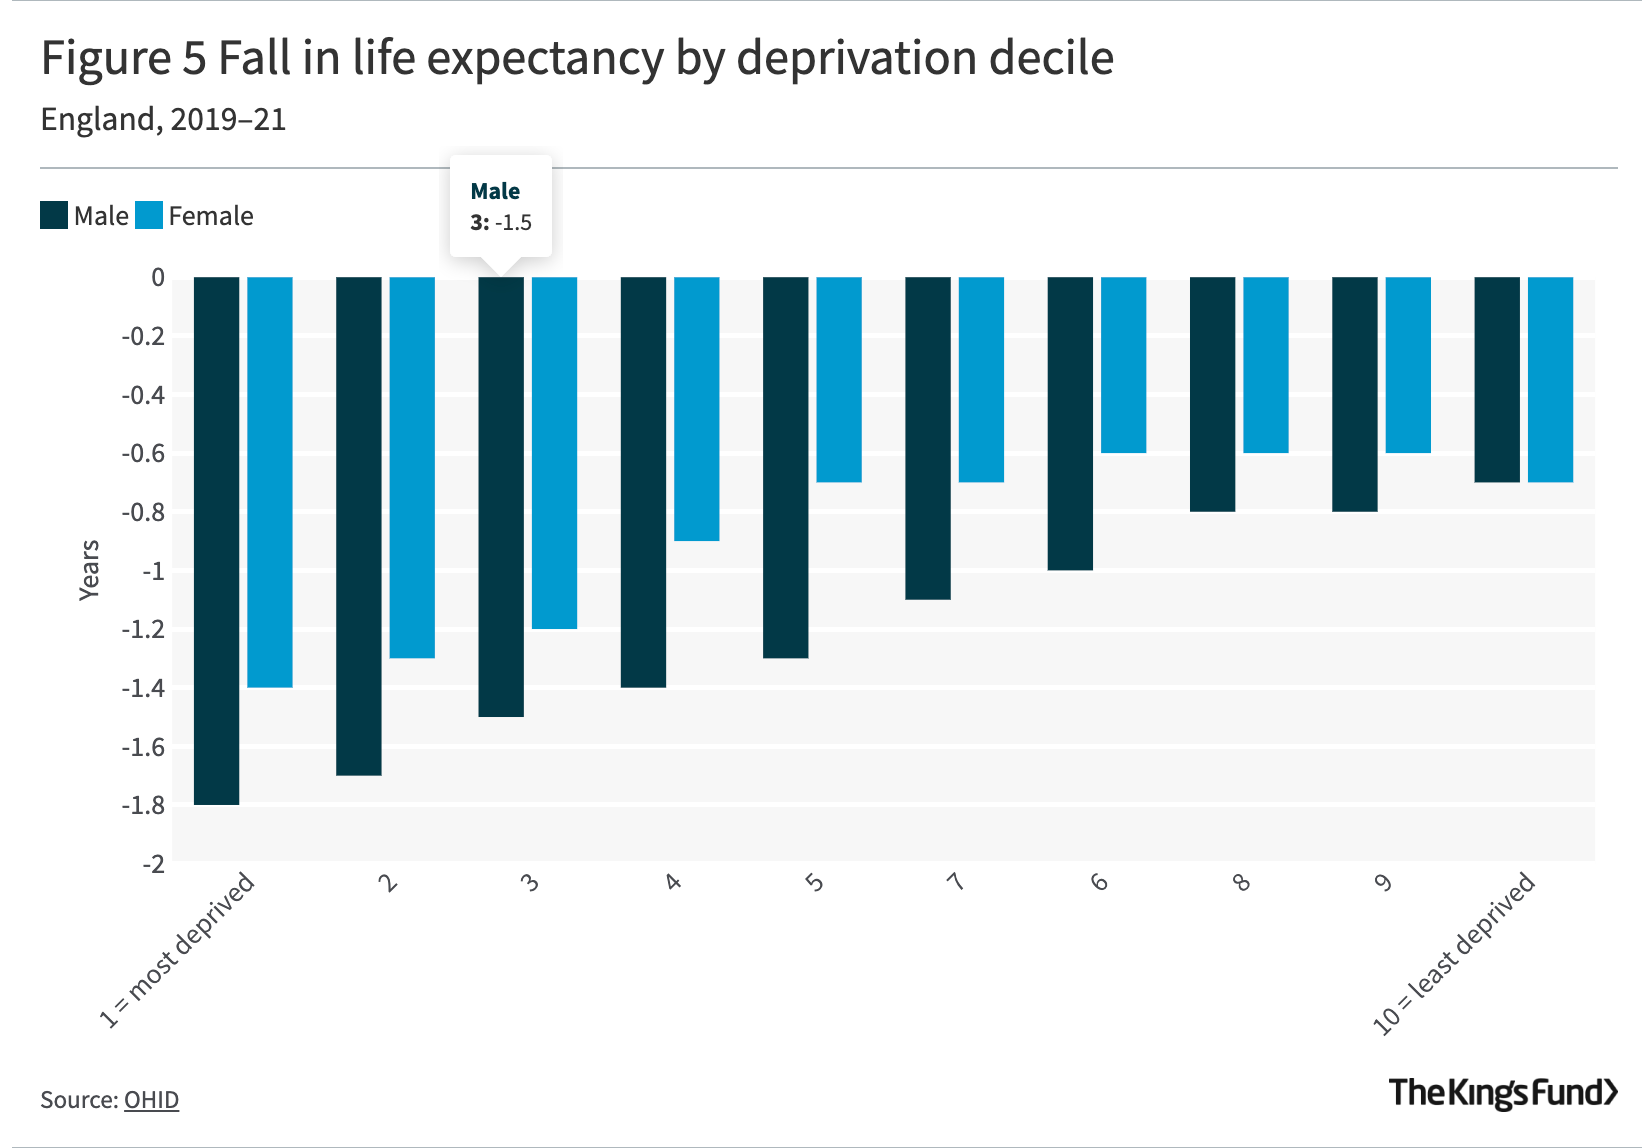
\includegraphics[width=4in]{images/ch3/33.png}
                \caption{Fall in life expectancy by deprivation decile, England, 2019-21}
            \end{figure}        
            During the Covid-19 pandemic, the most deprived male had a life expectancy drop of 1.8 years, while the least deprived male had a life expectancy drop of 0.7 years. Males tend to have a bigger drop than females. 

    \subsection{Why Do Health Disparities Exist?}\label{health_ineq_cause}

        Understanding the causes of health disparities is of key policy importance for addressing them (health subsidies, health information, nudge, for the poor people).
        
        \emphb{Potential Causes} are:
        \begin{enumerate}
            \item \empha{SES can causally affect health}. In terms of the Grossman model (Section \ref{grossman_demand}):
            \begin{itemize}
                \item Different SES groups (e.g. high vs. low education) can have different Marginal Efficiency of Health Capital (MEC):
                $$MEC\uparrow=MPH\times w\uparrow$$
                Thus, higher wage implies higher MEC, and hence higher equilibrium health stock.
                \item High SES individuals can have an expanded PPF because of extra financial resources.
                \item High SES individuals can have a lower rate of depreciation $\delta$ because of less stress. Thus, they will have a higher equilibrium health stock.
            \end{itemize}
            \item \empha{Early health can causally affect SES} (\emphb{Health Selection}).
            
            For example, unhealthy child $\to$ less educated $\to$ lower SES
            
            \item \empha{Both can be affected by third factors}.
            
            For example: time preferences (Fuchs’ hypothesis): people willing to delay gratification (high $\delta$) invest more in both health and education.
        \end{enumerate}

\section{Education and Health: Causal Inference}

    \subsection{Disparities by Education (Compulsory vs. Post-Compulsory)}
    
        \begin{figure}[H]
            \centering
            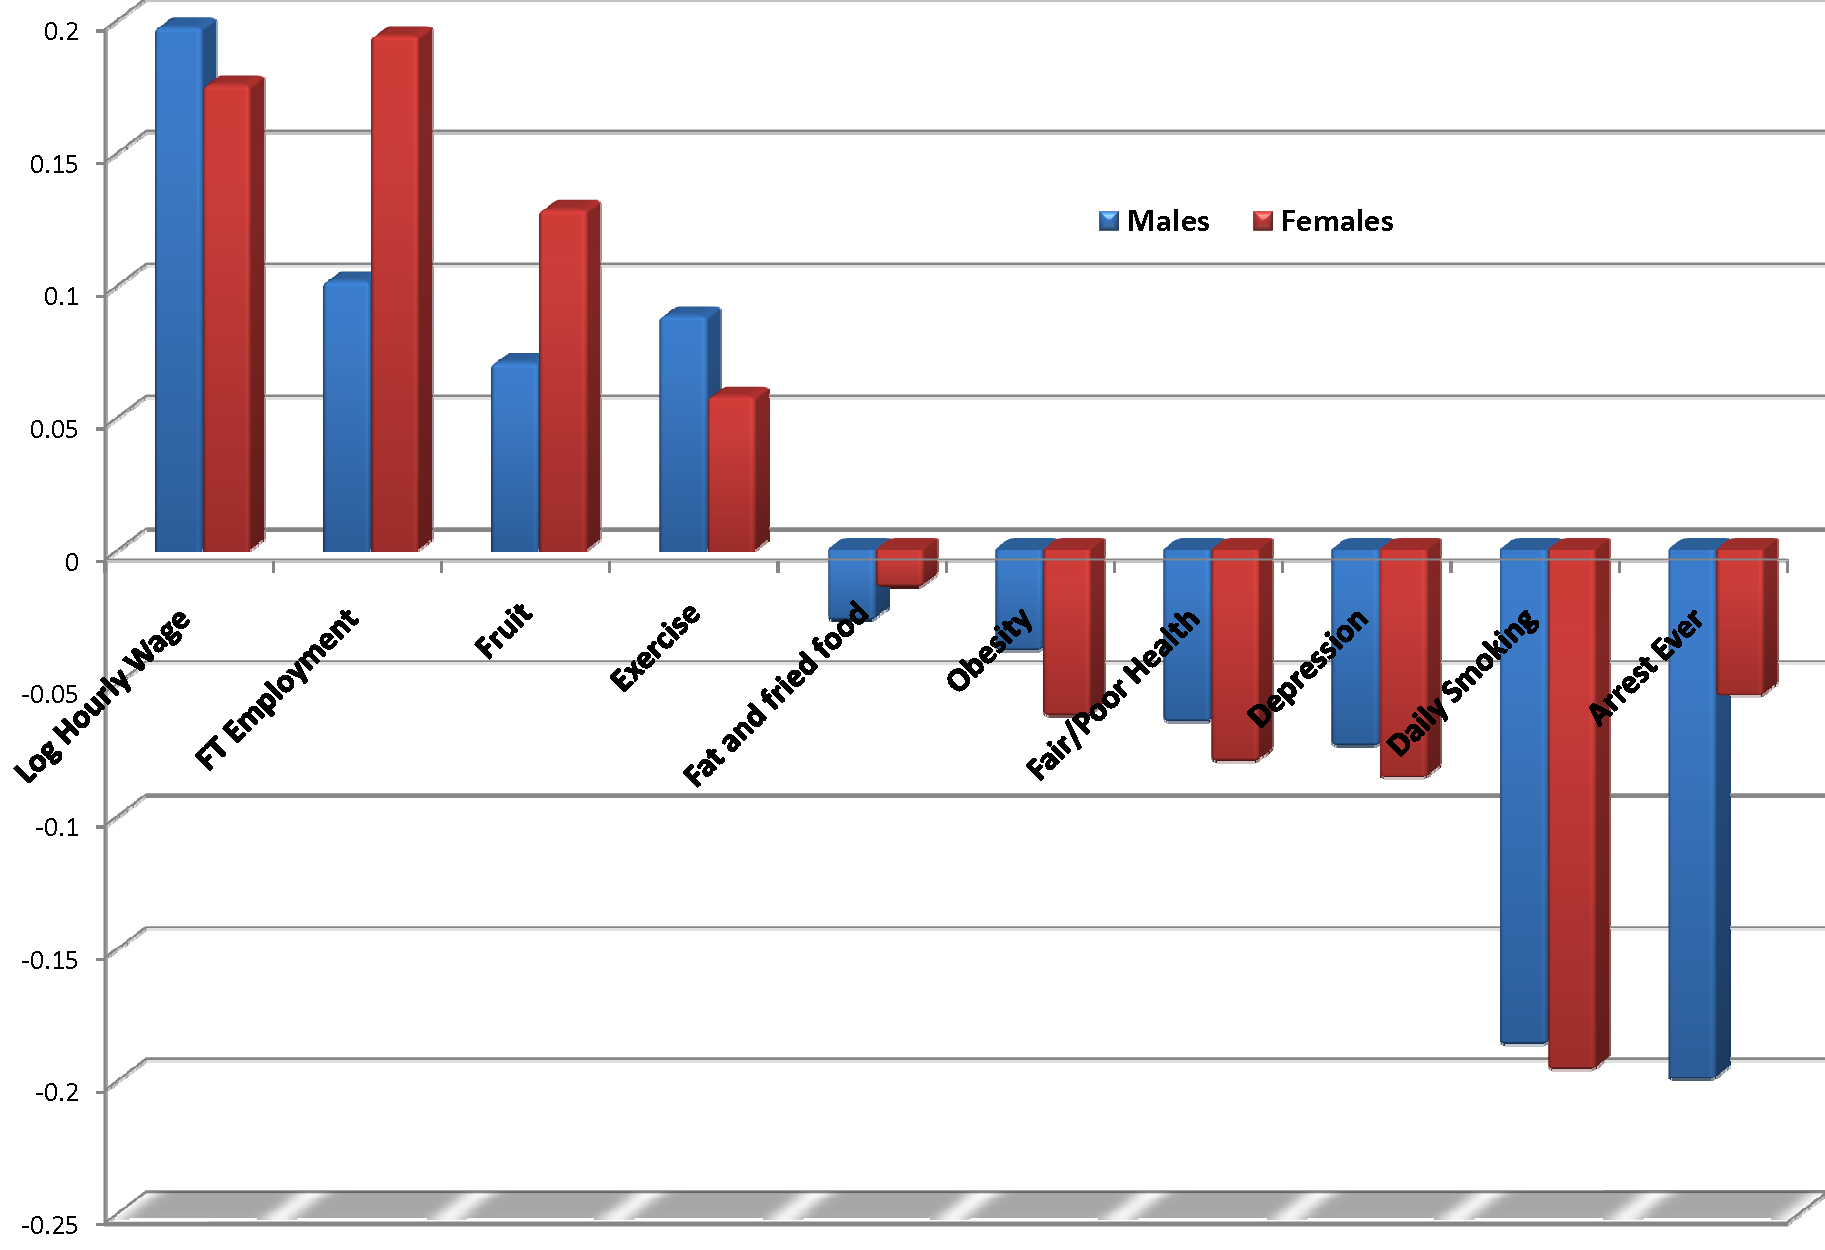
\includegraphics[width=4in]{images/ch3/34.png}
            \caption{Disparities by Education (compulsory vs. post-compulsory)}
        \end{figure}    
         The graph shows the raw differentials in the outcomes between individuals with post-compulsory and compulsory level of education.          Individuals with post-compulsory education tend to have better health.

    \subsection{Causality or Correlation? An Overview of Empirical Strategies}
    
        Key question: \empha{Is the positive correlation between health and schooling causal?}
        
        Literature has used different approaches to establish causality:
        \begin{itemize}
            \item First set of studies: used \emphb{instrumental variables} with questionable instruments for education (e.g. quarter of birth), finding strong effects.
            \item Second set of studies: exploited \emphb{features of the educational system}:
            \begin{itemize}
                \item Lleras-Muney (RevStud, 2005) uses compulsory school and child labour laws in thirty states from 1915 to 1939 as instruments for education and finds a significant effect in reducing mortality (using \emphb{DiD}).
                \item Clark and Royer (AER, 2013) use regression discontinuity methods (\emphb{RDD}) exploiting two changes to British compulsory schooling laws and find no effects on mortality or other measures of health (discussed in detail in Section \ref{clark_royer_RDD}). Similar results in a recent paper by Janke, Johnston, Propper et al. (JHE, 2018).
            \end{itemize}
            \item Third set of studies: \emphb{twin differences} (different between twins, NOT DiD!) (Lundborg, JPopEc 2013). Discussed in detail in Section \ref{lundborg_twin_diff}.
            \item Fourth set of studies: more “\emphb{structural}” models (Conti et al., 2010a,b; Heckman et al., 2018).
        \end{itemize}

    \subsection{Clark and Royer: RDD (AER, 2013)}\label{clark_royer_RDD}
    
        \subsubsection{Setup}
            \begin{figure}[H]
                \centering
                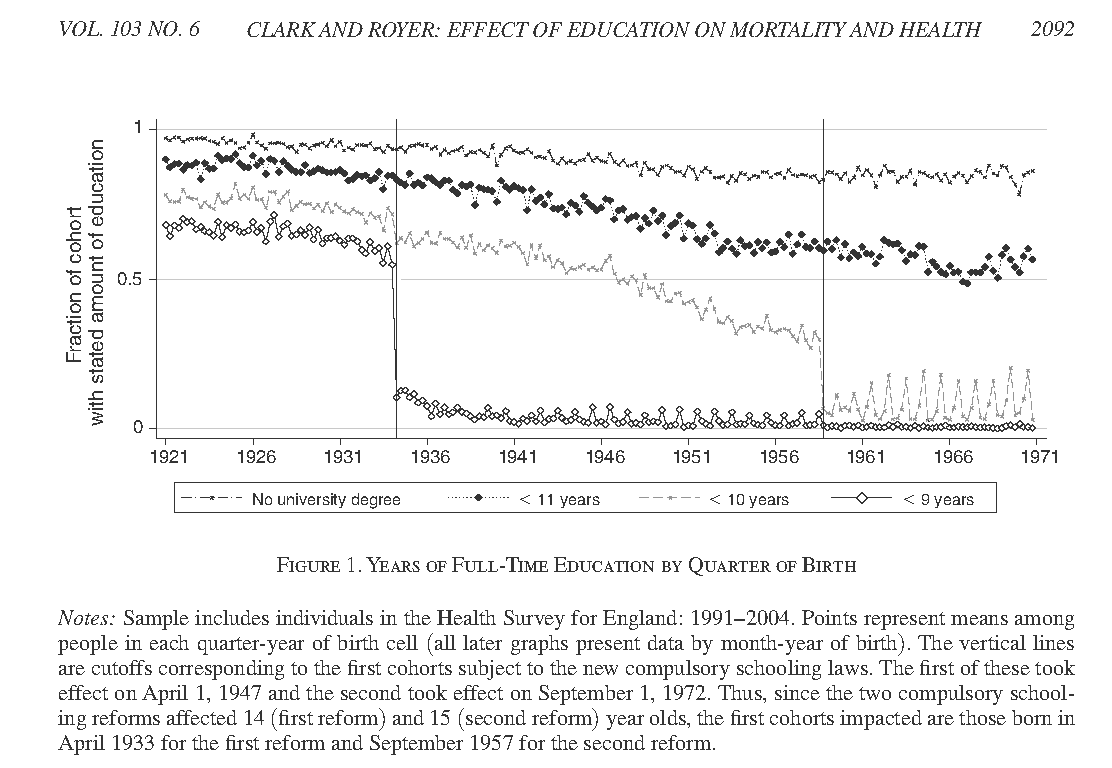
\includegraphics[width=5in]{images/ch3/35.png}
                \caption{Years of Full-Time Education by Quarter of Birth}
            \end{figure}
            This figure presents data at the quarter-of-birth level using Health Survey of England data. We study how the introduction of \emphb{two compulsory schooling laws} affected the fraction of cohorts with stated \emphb{amount of education}:
            \begin{itemize}
                \item The first reform took effect on April 1, 1947, which increased the compulsory school leaving age from 14 to 15.
                \item the second took effect on September 1, 1972, which increased the compulsory school leaving age from 15 to 16.
            \end{itemize}
            The vertical lines are cutoffs corresponding to the first cohorts subject to the new compulsory schooling laws. Since the two compulsory schooling reforms affected 14 (first reform) and 15 (second reform) years old, the first cohorts impacted are those born in April 1933 for the first reform and September 1957 for the second reform.
                     
            The 1947 change reduced the fraction that completed nine years or less by roughly one half; the 1972 change decreased the fraction that completed ten years or less by roughly one quarter. Hence, the reforms did increase students' years of education and \emphb{reduce the number of students who dropped out at a particular age.}

        \subsubsection{Discontinuity of the Running Variable}
            \begin{figure}[H]
                \centering
                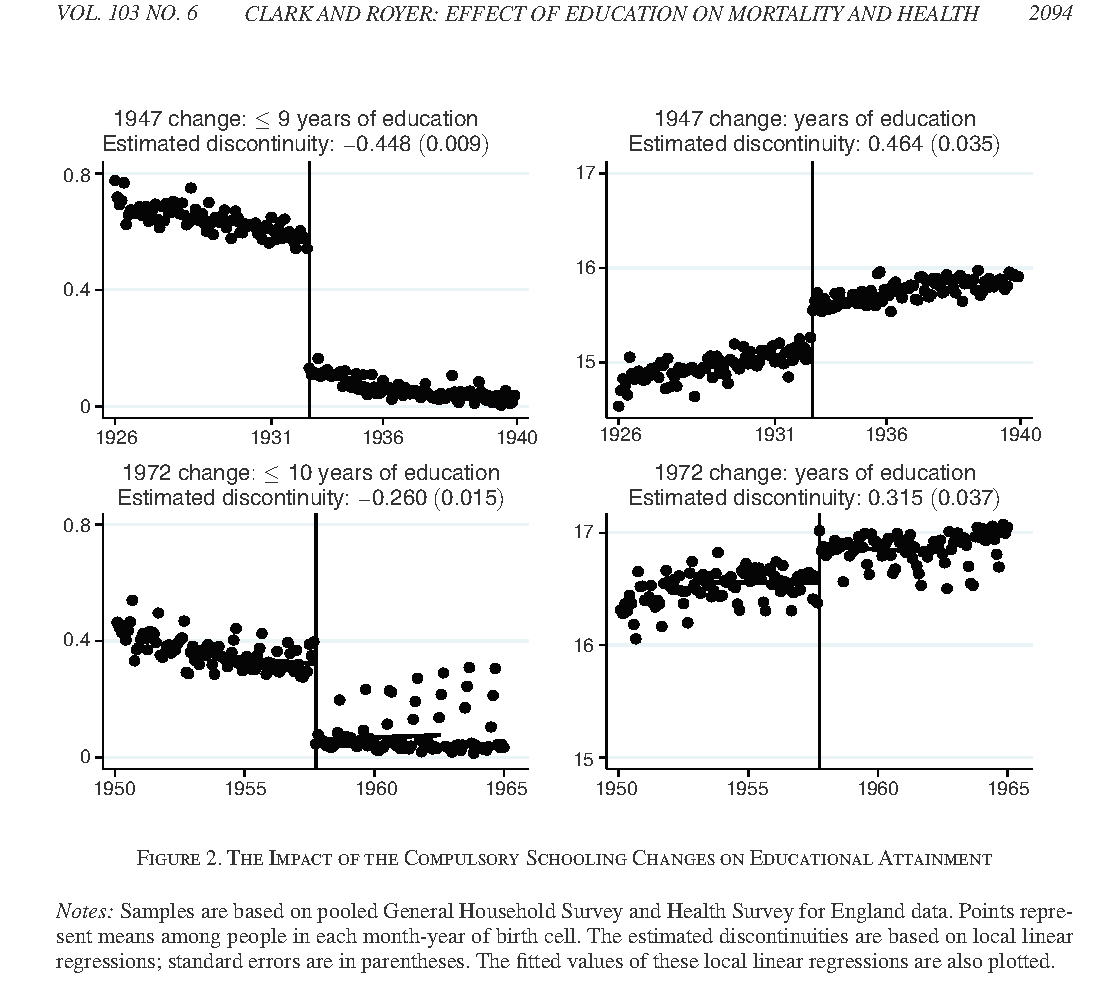
\includegraphics[width=4in]{images/ch3/36.png}
                \caption{The Impact of the Compulsory Schooling Changes on Educational Attainment}
            \end{figure}
            Here, our running variable is the \emphb{probability of completing certain years of education}.
    
            Specifically:
            \begin{itemize}
                \item To examine the effect of the law changes on educational attainment, we begin by graphing the relationship between the birth cohort and the probability of completing less than nine and less than ten years of education.
                \item The 1947 change reduced the fraction of individuals completing nine or fewer years of education by around 0.5. The 1972 change decreased the fraction completing ten or fewer years of education by around 0.25.
                \item The 1947 change increased the years of education of the 1933 cohort by around 0.5 years. The 1972 change increased the years of education of the 1957 cohort by around 0.3 years.
            \end{itemize}

        \subsubsection{Outcome}
            \begin{figure}[H]
                \centering
                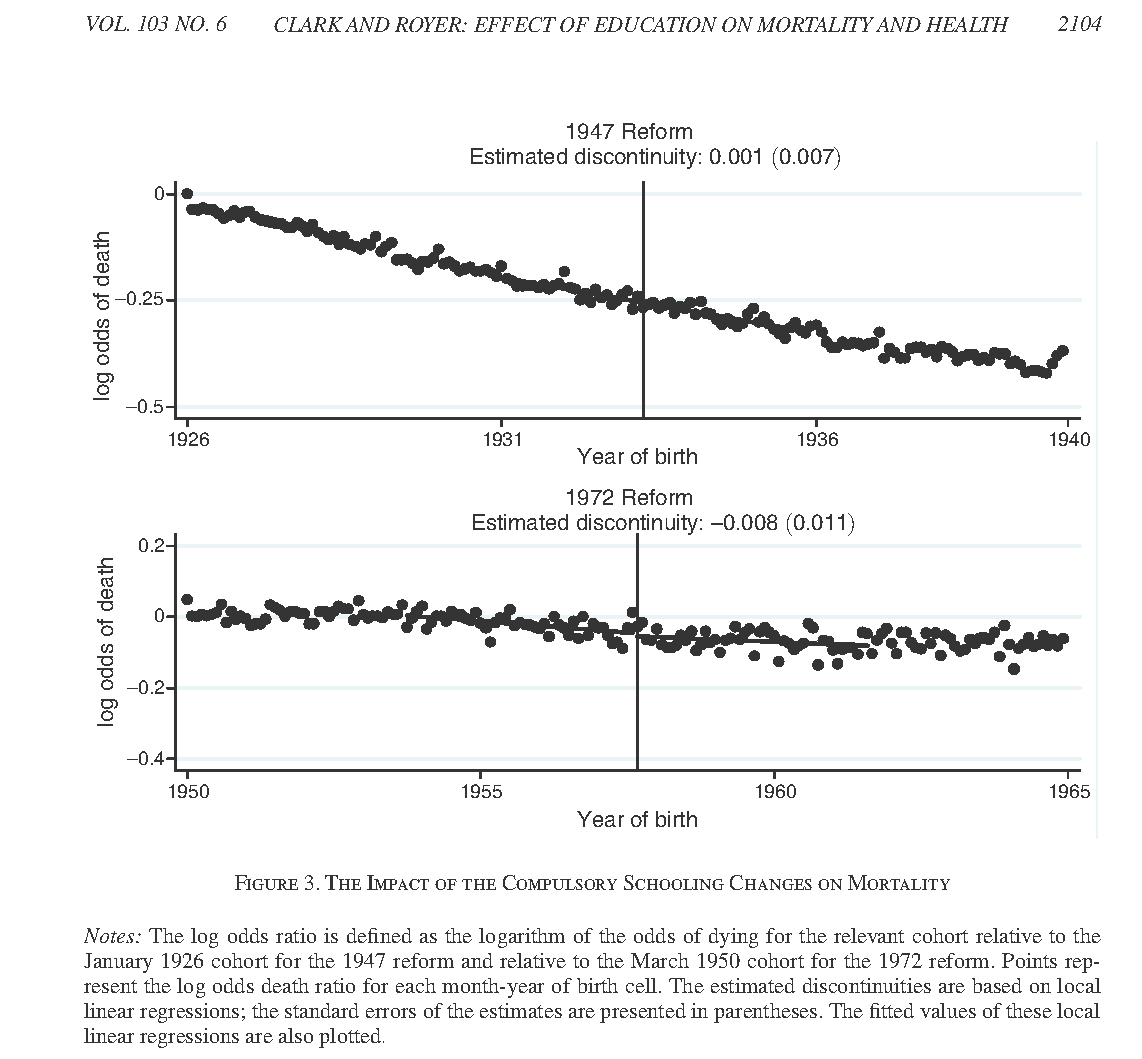
\includegraphics[width=4in]{images/ch3/37.png}
                \caption{The Impact of the Compulsory Schooling Changes on Mortality}
            \end{figure}

            Outcome variable 1: \emphb{mortality}: The two compulsory schooling laws have no effect on mortality (no discontinuity).
     
            \begin{figure}[H]
                \centering
                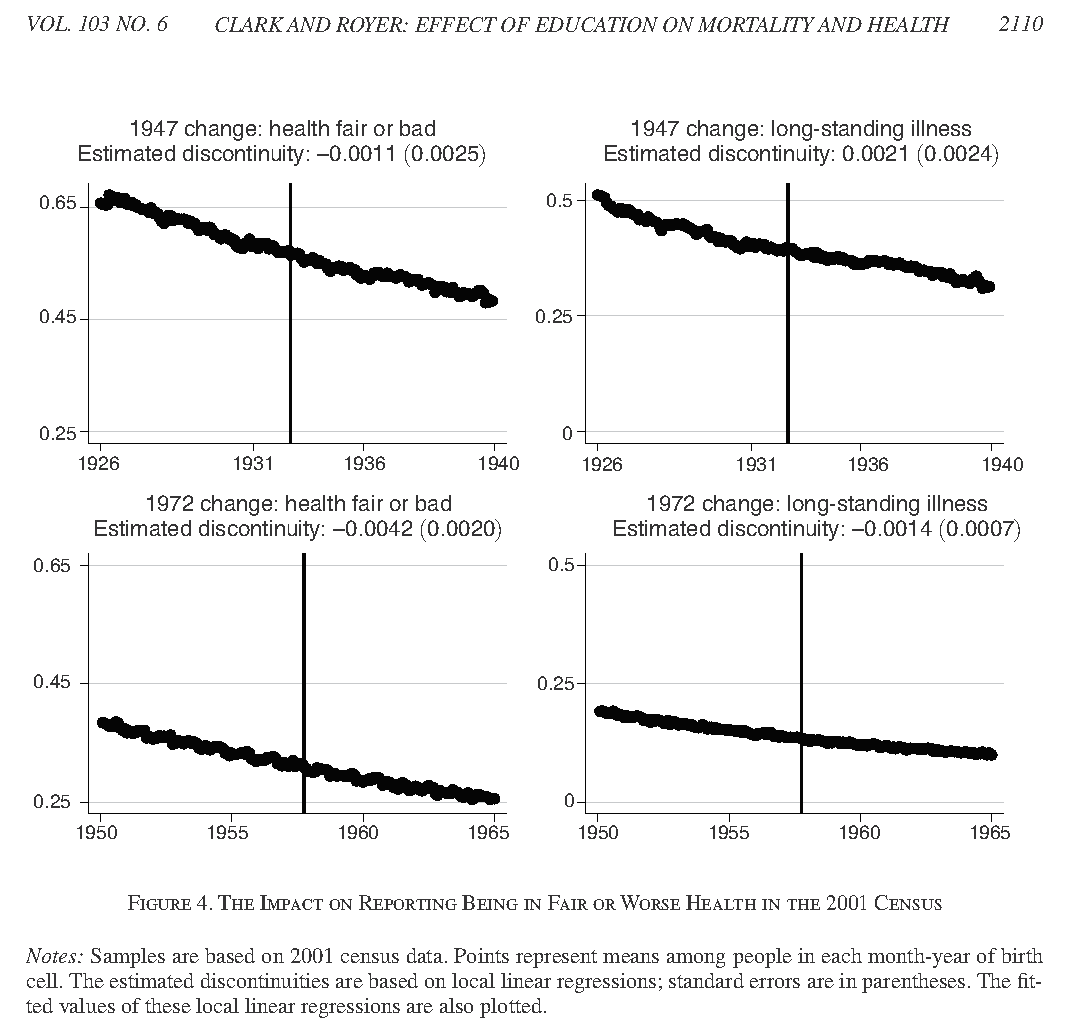
\includegraphics[width=4in]{images/ch3/38.png}
                \caption{The Impact on Reporting Being in Fair or Worse Health in the 2001 Census}
            \end{figure}  
            
            Outcome variable 2: \emphb{health fair or bad and long-standing illness}: The reforms cause no change in health fair or bad and long-standing illness.


            \begin{figure}[H]
                \centering
                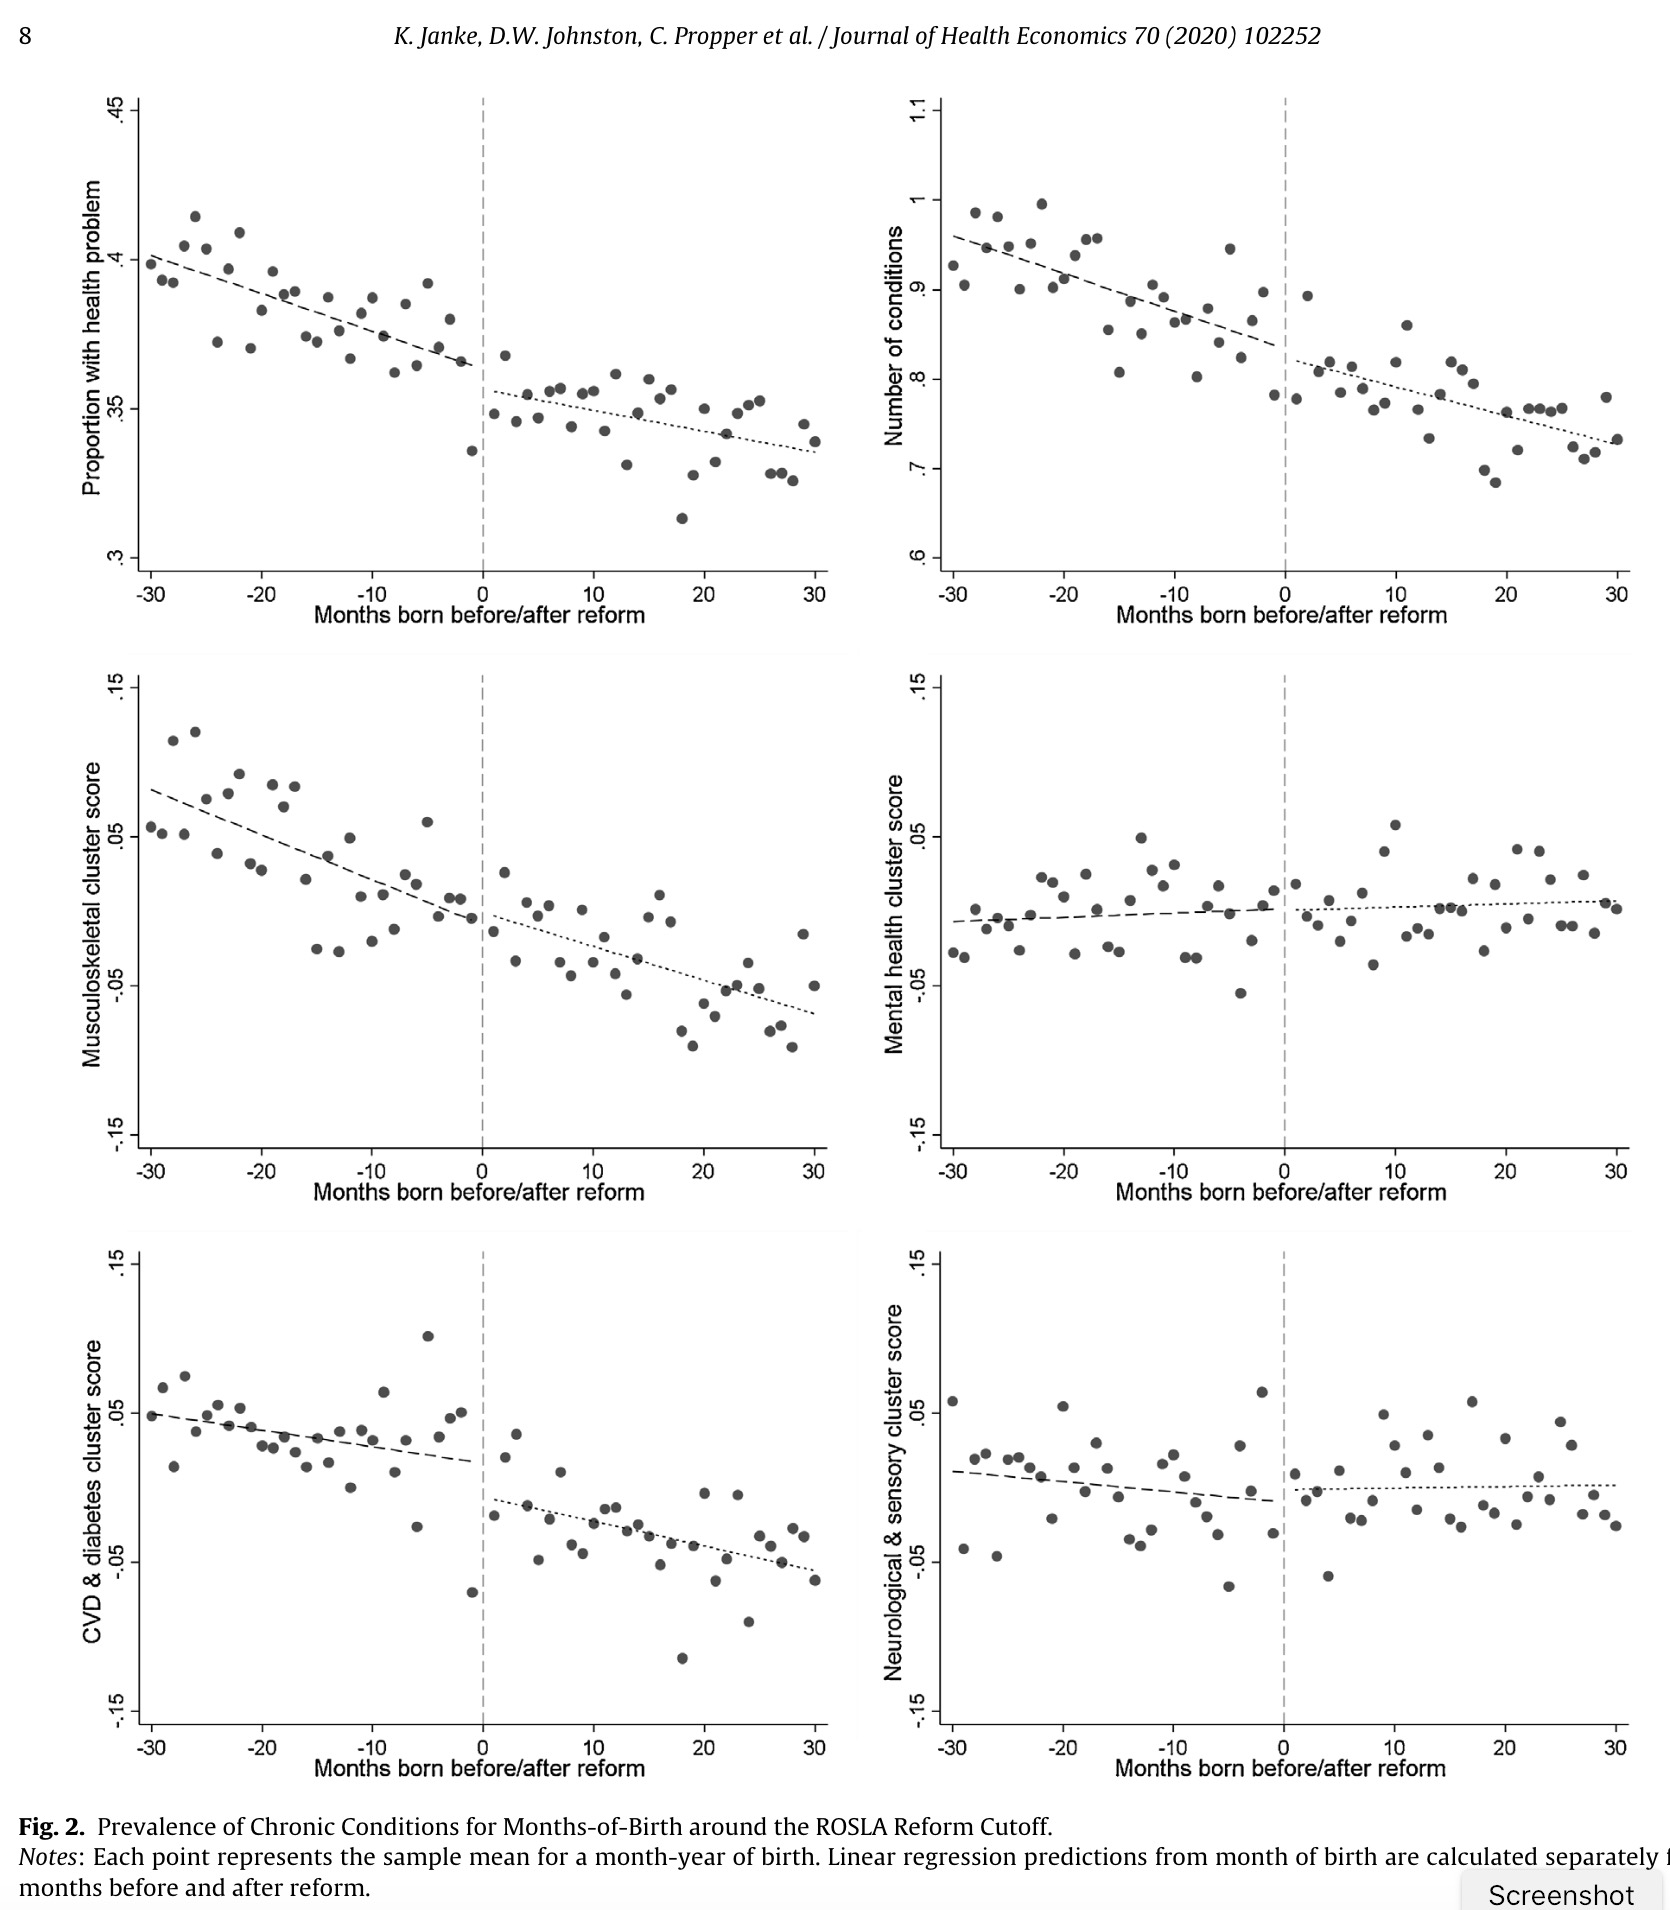
\includegraphics[width=4in]{images/ch3/39.png}
                \caption{Prevalence of Chronic Conditions for Months-of-Birth around the ROSLA Reform Cutoff}
                \label{fig:rosla_plot}
            \end{figure} 

            \emphb{Other outcome variables}: Another recent paper did the same reform and showed that only the prevalence of cardiovascular diseases was affected by the reform.

        \subsubsection{Conclusion}
            \empha{Higher education attainment shows nearly no effect on health conditions (at least at the cutoff).}

        \subsubsection{Extension: What If We Run an OLS?}
            \begin{figure}[H]
                \centering
                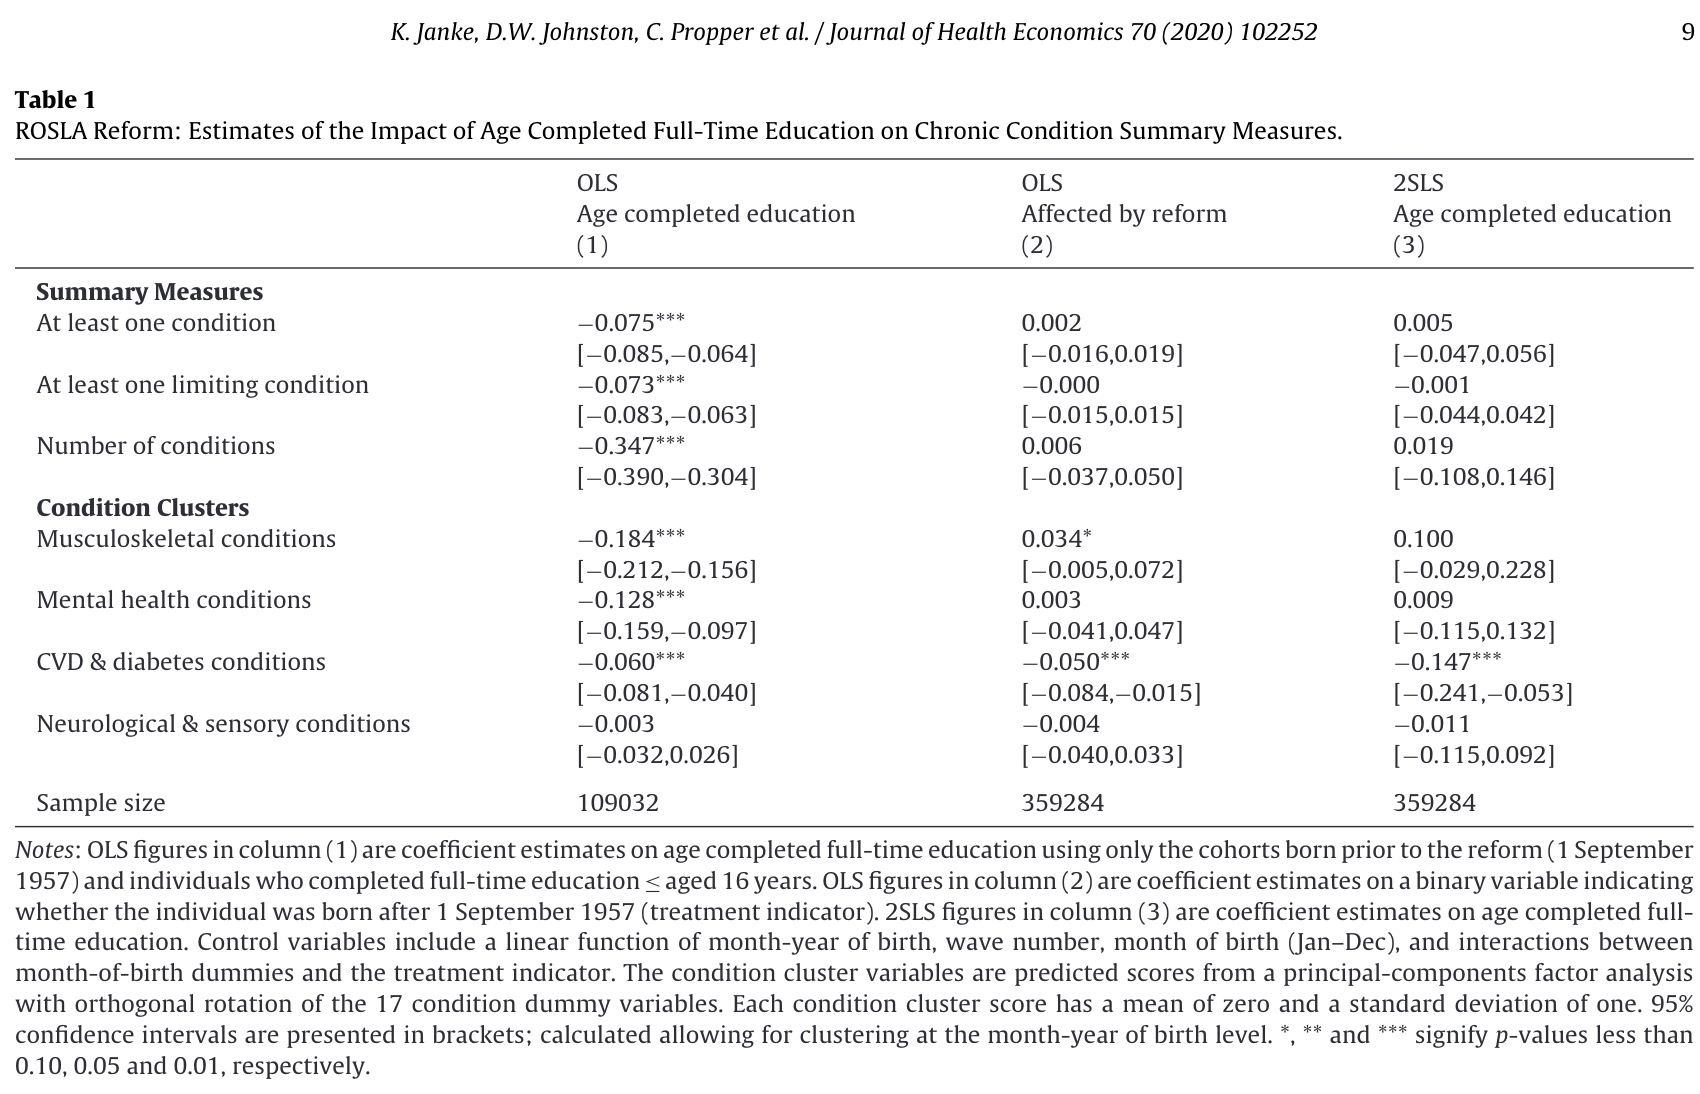
\includegraphics[width=5in]{images/ch3/40.png}
                \caption{ROSLA Reform Estimates}
            \end{figure}        
            If we directly run an OLS regression of education on health, we can see significant correlations. However, if we use 2SLS (Fuzzy RDD), we see that the coefficients are close to 0.

    \subsection{Lundborg, Journal of Population Economics 2013: Twin Differences}\label{lundborg_twin_diff}
        
        \subsubsection{Education (Endogenous)}
            $$Y_i = \alpha_0+\alpha_1 eduyrs_i+\alpha_2 X_i+\eta_i$$
                    where  $Y_i$ is the BMI of one twin
            
            Take the difference between twins' BMIs:
            
            $$\Delta Y = \beta_0+\beta_1\Delta eduyrs+\beta_2 \Delta X+\Delta \eta$$
            where  $\Delta Y=Y_i-Y_j$ 
            
            This is a fixed-effect regression.
            
            However, $\beta_1$ will not be interpreted as the causal effect of education on health, as education is a choice, which is likely to be correlated with the error term (ability/effort/parents' investment), so we need an instrument for $\Delta eduyrs$.
        
        \subsubsection{Birth Weight (Exogenous)}
            However, if we estimate
            
            $$\Delta Y = \gamma_0+\gamma_1\Delta BW+\gamma_2 \Delta X+\Delta \eta$$
            
            where BW is the birth weight,
            
            $\gamma_1$ identifies the causal effect of birth weight difference on BMI difference, as birth weight is predetermined.





\subsection{Explaining the Gradient}
\begin{enumerate}
    \item Cutler and Lleras-Muney (JHE, 2010)

\begin{itemize}

        \item Cutler and Lleras-Muney (JHE, 2010) examine possible explanations for the relationship between education and health, using several datasets from US and UK. They use OLS regression and see \emphb{how much the coefficient goes down when adding additional covariates}.
        \item They are able to explain two-thirds of the gradient.
        \item "Economic resources" is able to explain 32 percent of the gradient. "Specific knowledge" is able to explain 12 percent of the gradient (US dataset). "Cognitive ability" seems to explain a lot in the UK dataset. "Tastes" and "Personality" explain a little and "social integration" explains somehow.
\end{itemize}
        
\begin{figure}[H]%option [H] means "strictly here"
                \centering
                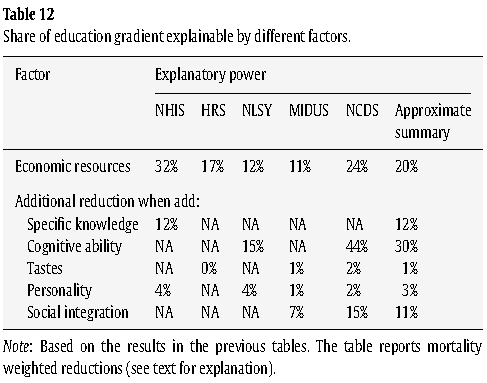
\includegraphics[width=4in]{images/ch3/41.png}
                \caption{Share of education gradient explainable by different factors}
            \end{figure}
            
\item Conti and Hansman (JHE, 2013)
            
\begin{itemize} 
        \item Conti and Hansman (JHE, 2013) test the robustness of Cutler and Lleras-Muney's (CLM) results by using alternative measures of child personality available in the National Child Development Study:
\begin{itemize}
        \item the Rutter Behavior Scale (ages 7, 11 and 16)
        \item the British Social Adjustment Guide (BSAG, ages 7 and 11):
\end{itemize}
        \item CLM results show that adult personality explains very little of the education-health gradient, but Conti and Hansman (JHE, 2013) show that child personality contributes the education-health gradient to an extent nearly as large as cognition. 
        \item Childhood matters.
\end{itemize}
\begin{figure}[H]%option [H] means "strictly here"
                \centering
                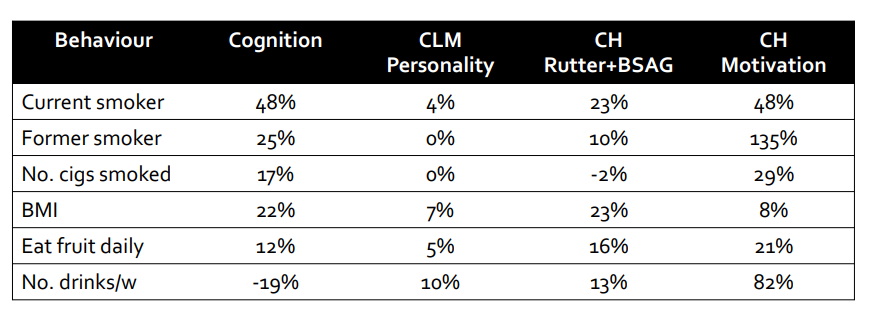
\includegraphics[width=4in]{images/ch3/42.png}
                \caption{How much education-health gradient is explained by cognition, personality and motivation}
            \end{figure} 
\end{enumerate}


\subsubsection{Child Socioemotional Traits Are Important Determinants of the Gradient}
\begin{figure}[H]%option [H] means "strictly here"
                \centering
                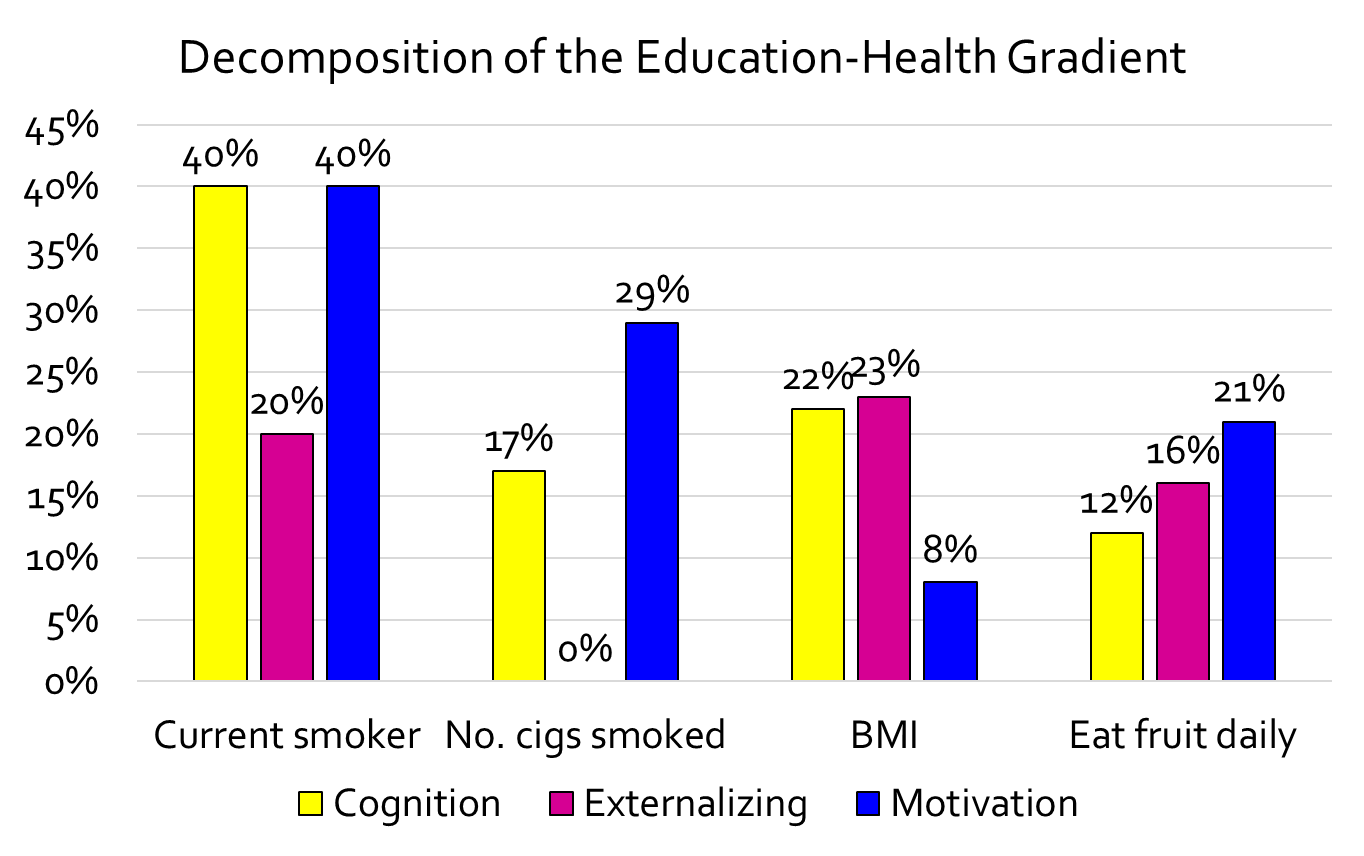
\includegraphics[width=4in]{images/ch3/43.png}
                \caption{Decomposition of the Education-Health Gradient}
            \end{figure} 

\begin{itemize}
        \item Non-cognitive factors such as externalising and motivation are at least as important as cognition in explaining the gradient.
\end{itemize}

\subsubsection{The Early Origins of the Gradient}

\begin{itemize}
        \item Conti, Heckman et al. (AER, PPS, 2010a,b) decompose observed educational differentials into causal components and components due to selection on early childhood human capital endowments.
        \item They incorporate both the health selection, the social causation and the third factors hypothesis.
        \item They look at the mean effect of education on health (like previous literature) and also at heterogeneity in treatment effects for people with different early childhood endowments.
        \item They quantify the proportion of the educational differential attributed to the causal effect of education vs. early life factors. 
        \item Heckman, Humphries and Veramendi (JPE 2018) extend this framework into a dynamic model of schooling choice and estimate causal effects from multiple levels of schooling. Find substantial continuation value of schooling for high-ability individuals, but not for low ones beyond high school.
        \item Conti et al. use the British Cohort Study (BCS70), a cohort of all individuals born in one week of April 1970 in the United Kingdom.
        \item They estimate a semiparametric structural model of the choice of schooling (decision to stay on at 16) and the causal effect of schooling on a variety of outcomes at age 30: 
        \begin{enumerate}
            \item labour market (wages and employment)
            \item health status (self-reported health, depression and obesity)
            \item health behaviours (smoking, exercise)
        \end{enumerate}
        \item They model three childhood (age 10) endowments as determinants both of education and age 30 outcomes:
        \begin{enumerate}
            \item cognition (e.g. British Ability Scales)
            \item noncognitive traits (e.g. locus of control)
            \item health (height, head circumference)
            \end{enumerate}
          \item We want these three early childhood factors to affect education (if the child is more developed $\Rightarrow$ more able to learn $\Rightarrow$ acquire more education).  Education affects health. Also, these three factors affect health directly. With this structure, health is partly causally affected by education, and partly causally affected by early childhood factors.

          
\begin{figure}[H]%option [H] means "strictly here"
                \centering
                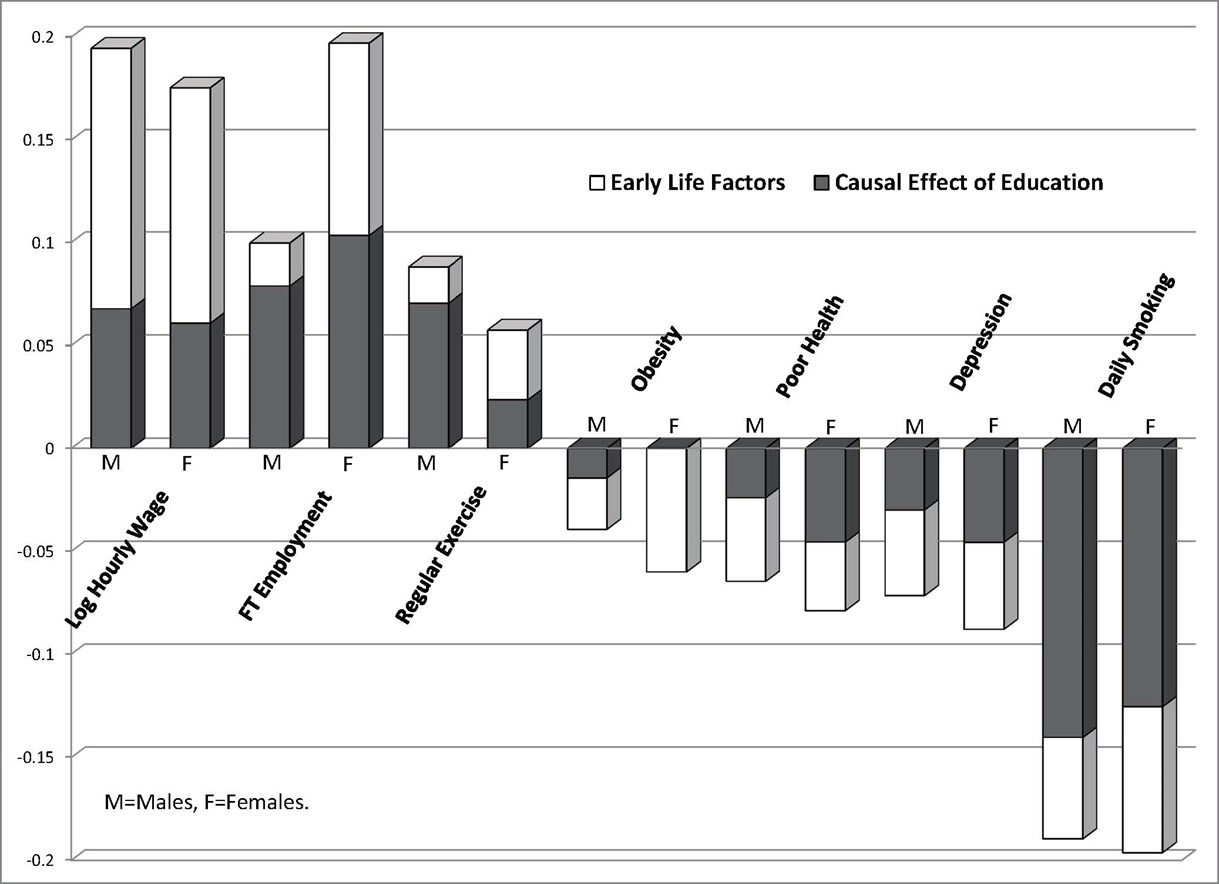
\includegraphics[width=4in]{images/ch3/44.png}
                \caption{How education and early life factors share the causal effects on different health outcomes}
            \end{figure}        
\end{itemize}

\begin{itemize}
\item Education explains nearly nothing about the obesity of females. For daily smoking, education matters more than early life factors.
\end{itemize}

\subsubsection{The Effects of Childhood Endowments on the Probability of being a Daily Smoker at Age 30}    
\begin{figure}[H]%option [H] means "strictly here"
                \centering
                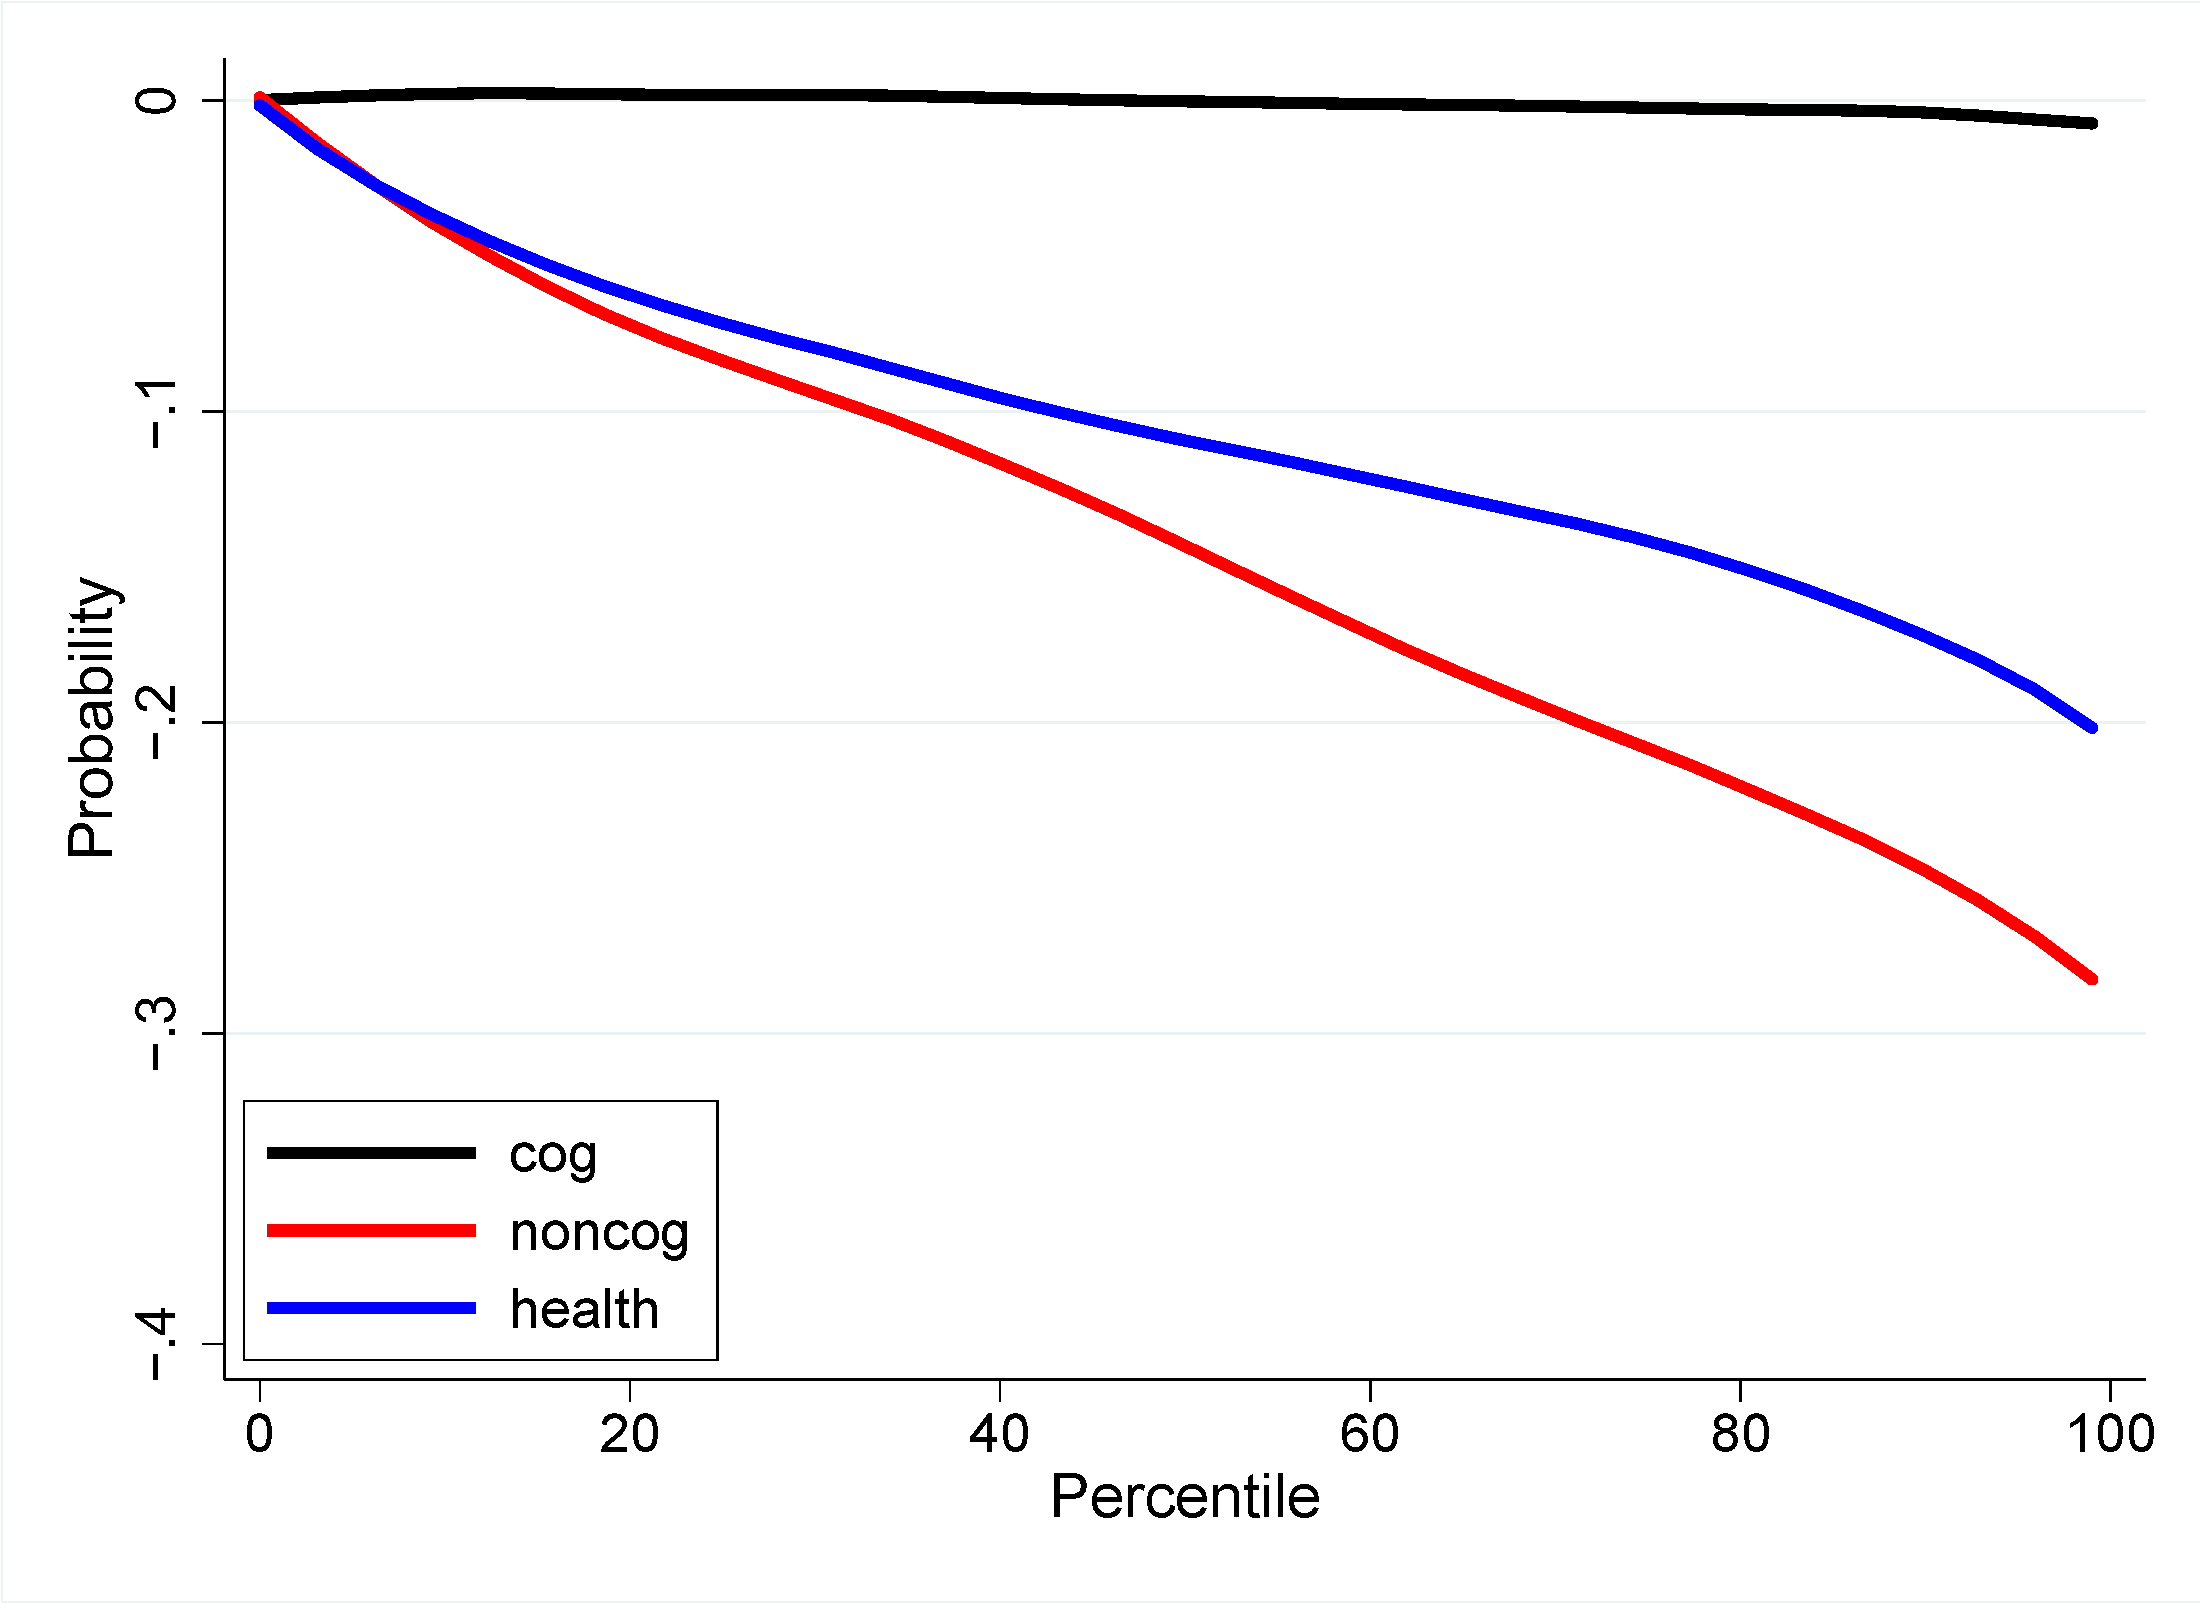
\includegraphics[width=4in]{images/ch3/45.png}
                \caption {The Effects of Childhood Endowments on the Probability of
being a Daily Smoker at Age 30}
            \end{figure} 

\begin{itemize}
    \item Cognition doesn't affect smoking. Non-cognitive factors (e.g. self-regulation and motivation) and physical health are equally important determinants of smoking.
\end{itemize}

\subsubsection{The Effects of Childhood Endowments on the Probability of being Obese at Age 30}    
\begin{figure}[H]%option [H] means "strictly here"
                \centering
                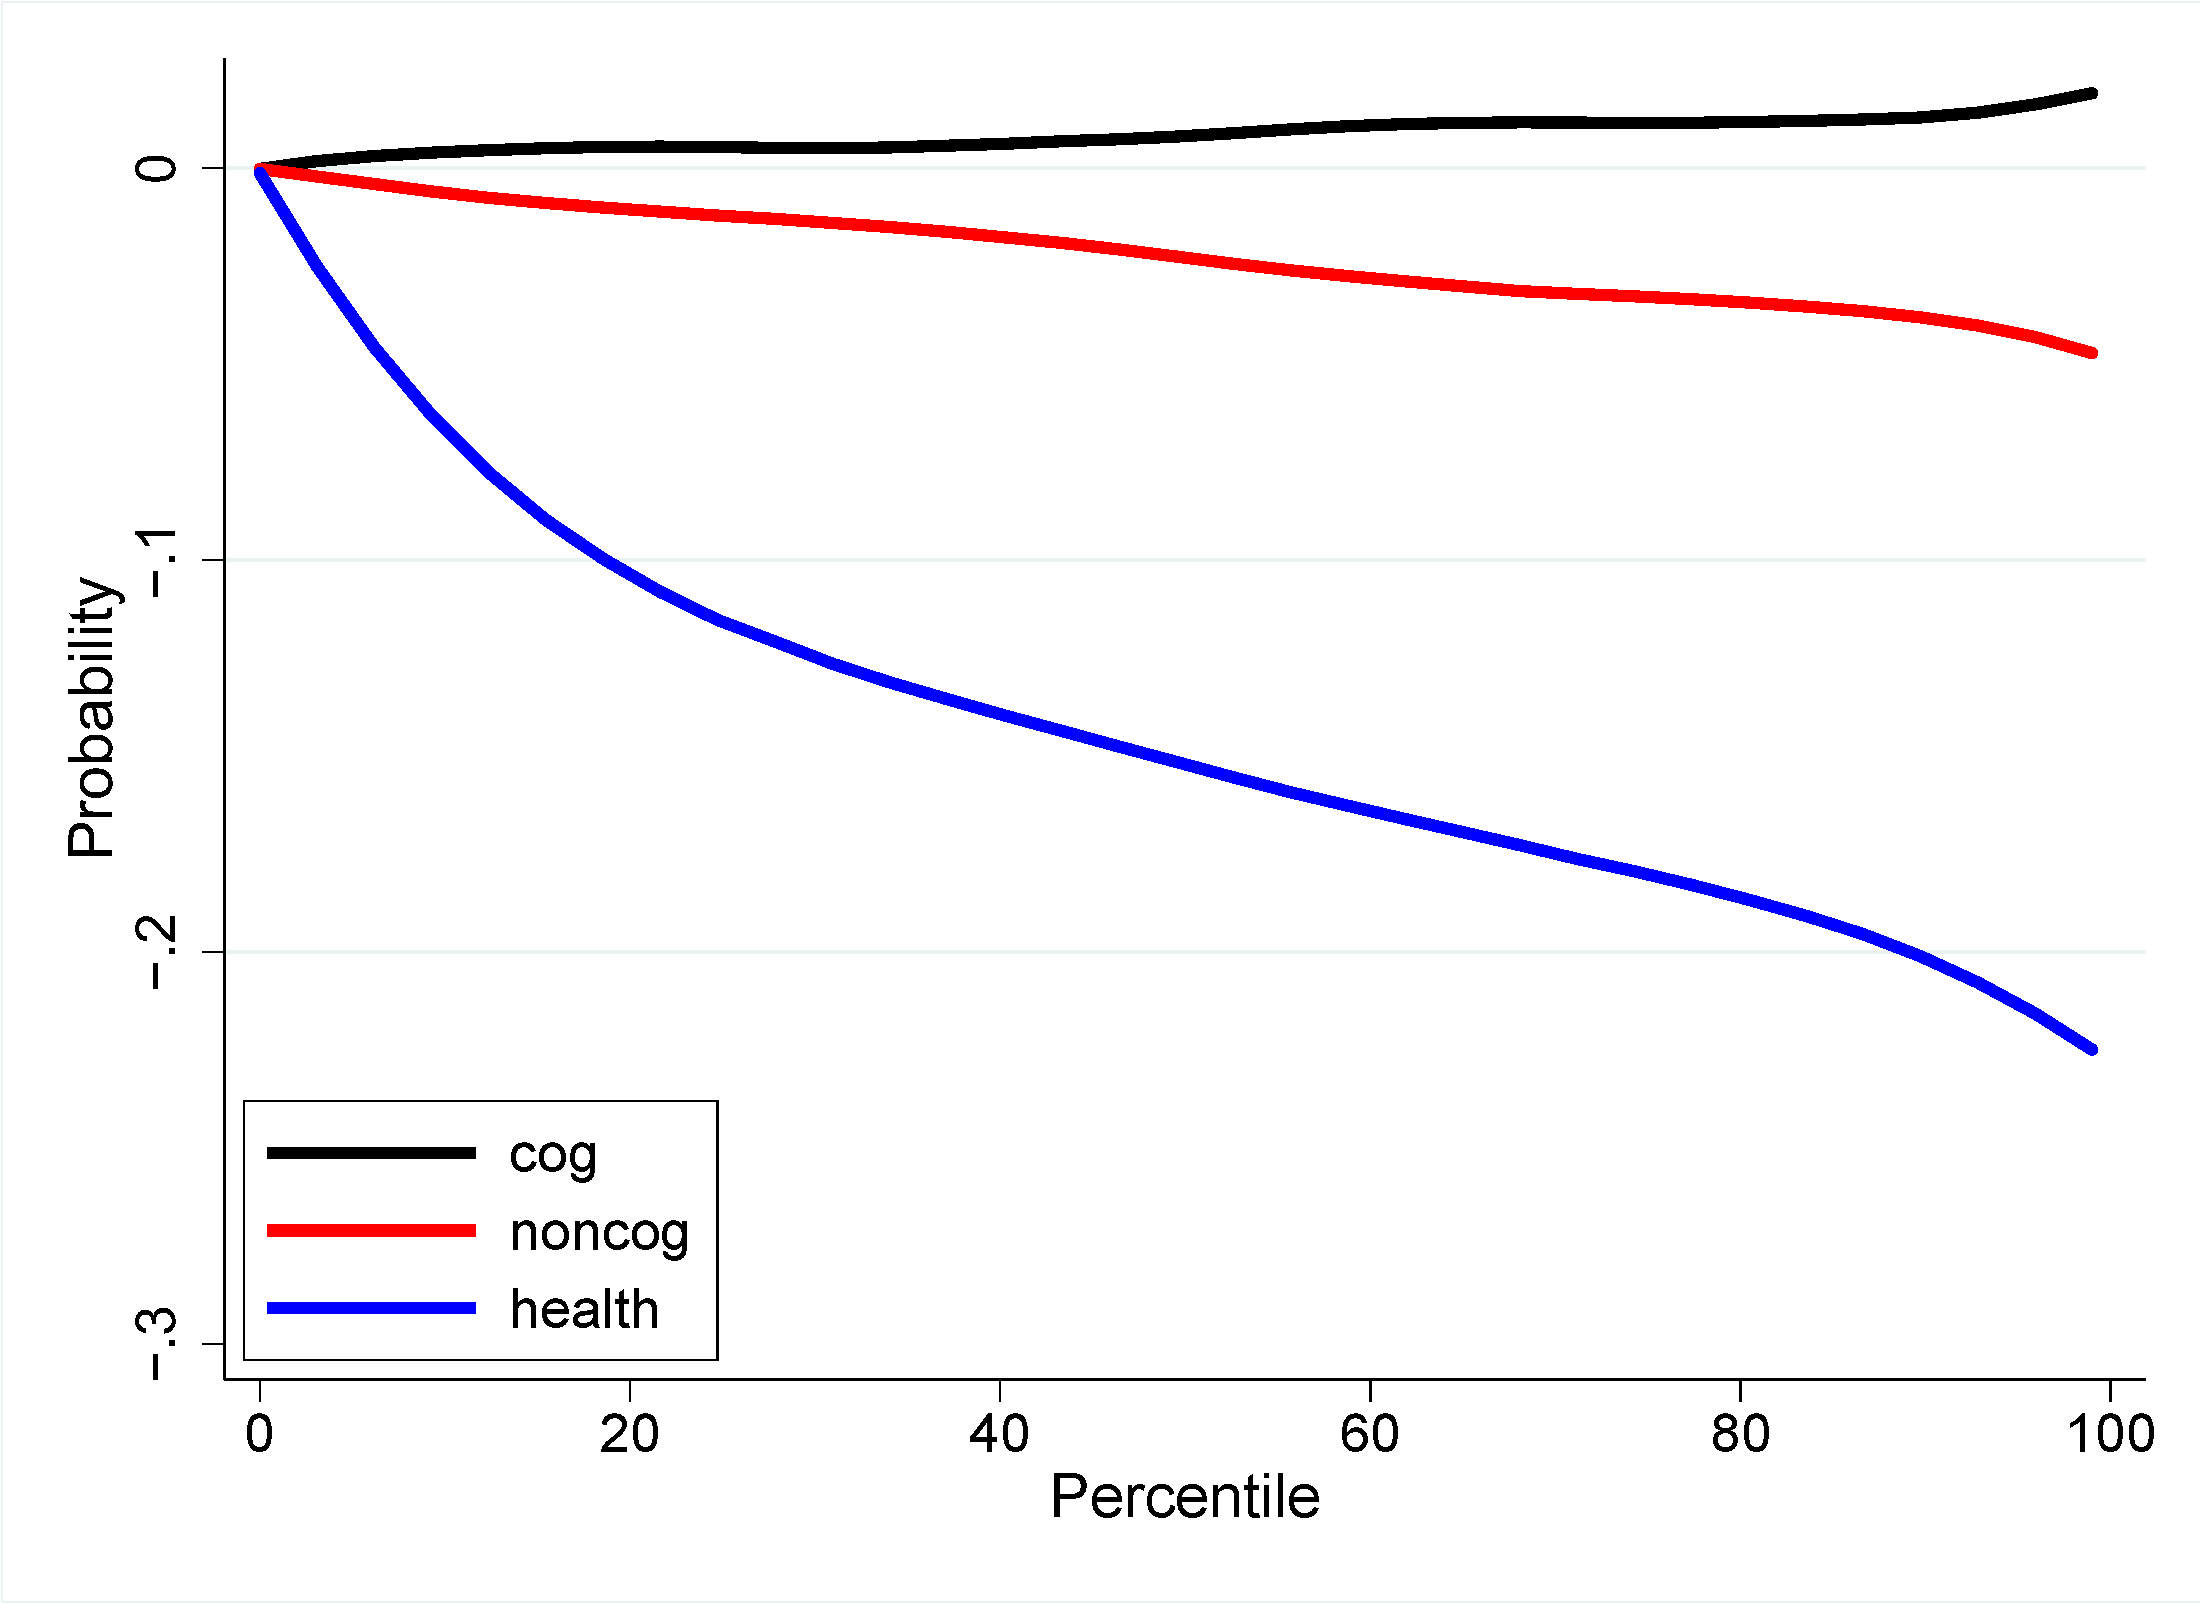
\includegraphics[width=4in]{images/ch3/46.png}
                \caption {The Effects of Childhood Endowments on the Probability of
being Obese at Age 30}
            \end{figure} 
            
\begin{itemize}
    \item Cognition matters little. Non-cognitive explains a little bit. Early physical health is the most important determinant of obesity.
\end{itemize}

\subsubsection{Heterogeneity in the Effects of Education on Smoking}    
\begin{figure}[H]%option [H] means "strictly here"
                \centering
                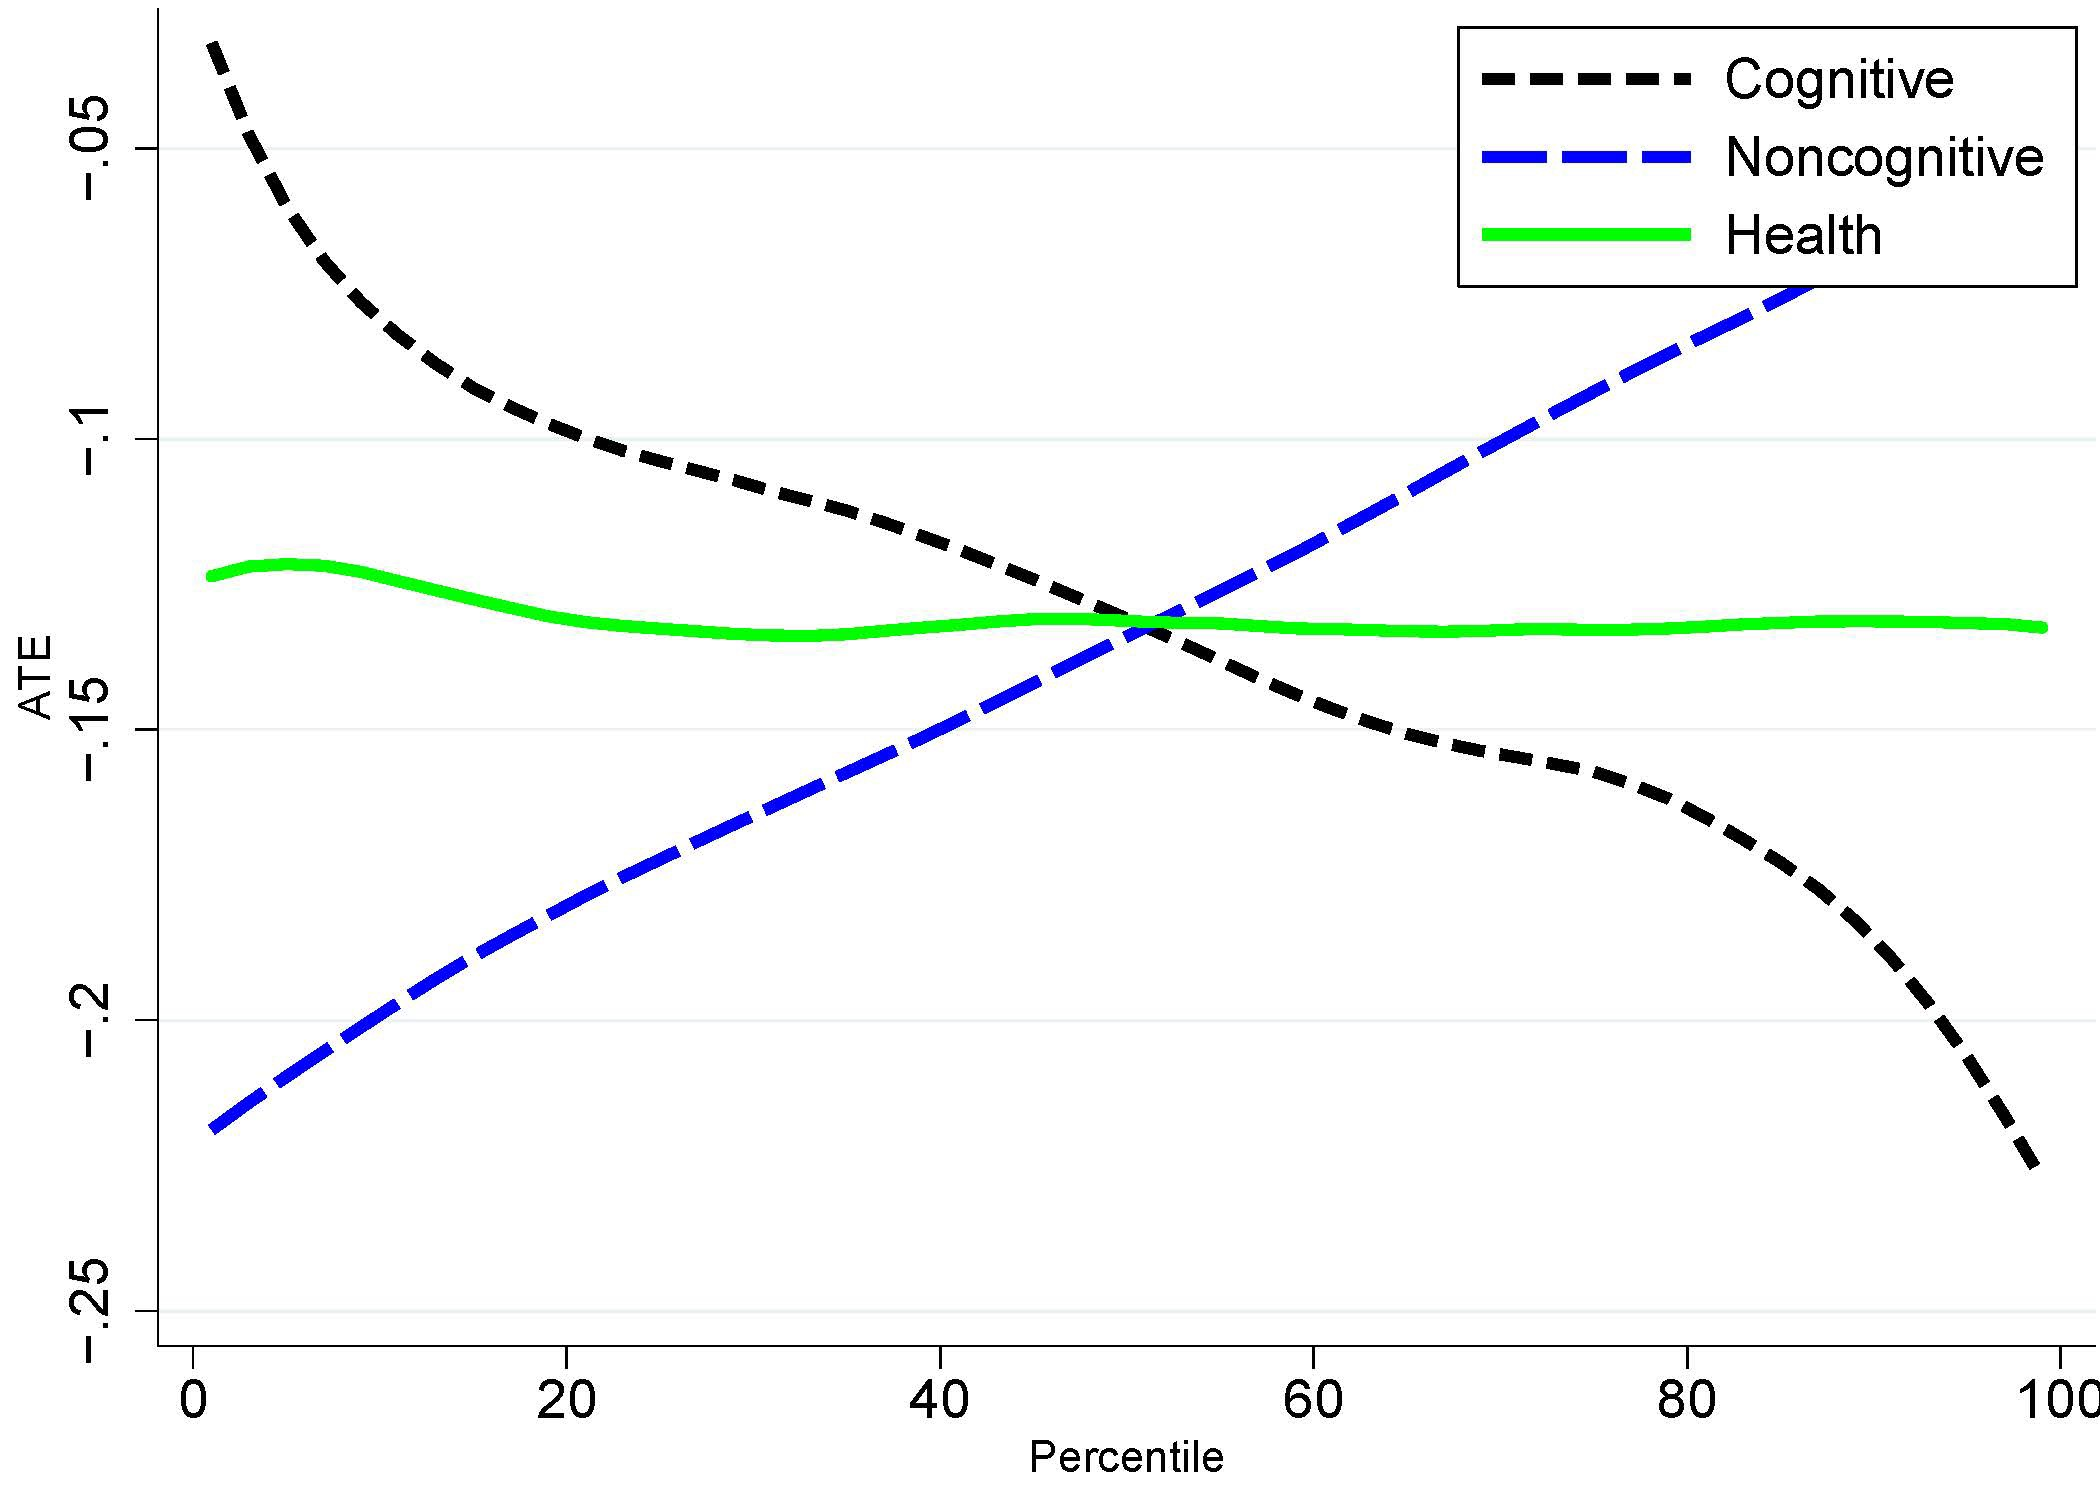
\includegraphics[width=4in]{images/ch3/47.png}
                \caption {Heterogeneity in the Effects of Education on Smoking}
            \end{figure} 
            
\begin{itemize}
    \item The effects of later intervention (education) on smoking depend on the effects of early child interventions.
    \item Heterogeneity in the effects (ATE=Average Treatment Effect) of post-compulsory education on smoking at age 30 as function of early endowments: education compensates for low early non-cognitive endowments and reinforces high early cognitive endowments.
    \item First, the beneficial effect of education (ATE) is much bigger at the top of the cognitive ability distribution. This is particularly interesting in the case of smoking, as it is consistent with the interpretation that the information content on the dangers of smoking provided by post-compulsory education needs to be combined with the capacity to process that information in order to be effective. Second,  education compensates for poor noncognitive ability (increase motivation). Third, there is no heterogeneity in the effect of education along the distribution of the health endowment. 
 
\end{itemize}

\subsubsection{Evidence from a Dynamic Model}  
\begin{figure}[H]%option [H] means "strictly here"
                \centering
                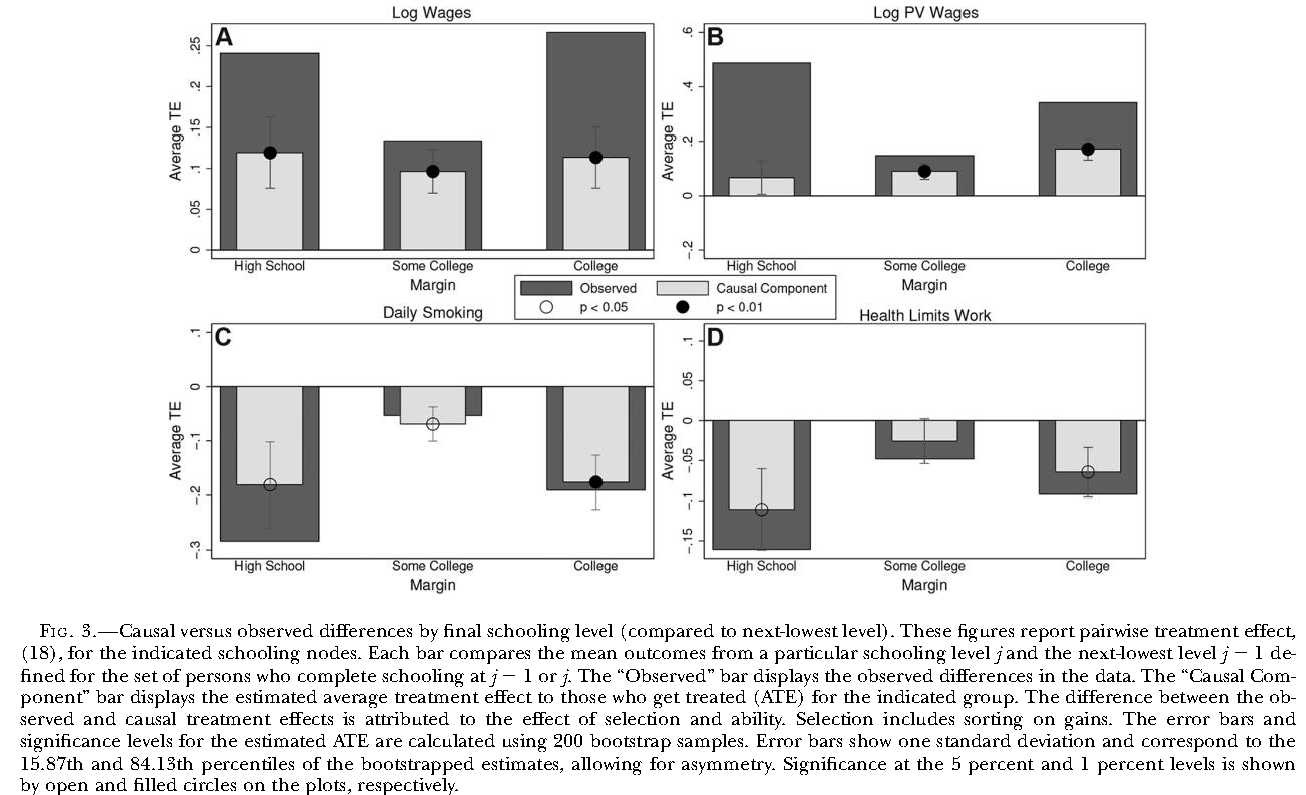
\includegraphics[width=5in]{images/ch3/48.png}
                \caption {Evidence from a Dynamic Model}
            \end{figure}
\begin{itemize}
    \item How additional level of education affects wages and health compared to previous education level
    \item The shaded regions labelled “Observed” are the raw differences found in the data. The estimated average causal effects (displayed in the light blocks) are large and statistically significant for all outcomes except for the log PV wages for graduating from high school (compared to dropping out). For example, the left-most bar in panel A can be interpreted as follows: while high school graduates make, on average, 24 log points higher wages than high school dropouts, we find that the average causal effect of graduating from high school is, on average, 12 log points for the same population.
    \item Panel C: The biggest reduction in smoking was seen in people with high school degrees compared to those without, and more than half of the effect can be explained by the causal effect of education. However, most of the reduction in smoking can be explained by the causal effect of education for people with college degrees compared to those without. The causal component depends on each level of education (as well as the quality of education).
\end{itemize}

            

\subsubsection{The State of the Literature}  
\begin{itemize}
    \item Recent review “The Effect of Education on Health and Mortality: A Review of Experimental and Quasi-Experimental Evidence” by T. Galama, A. LlerasMuney, H. van Kippersluis, Oxford Research Encyclopedia of Economics and Finance (2018).
    \item Review evidence on the two most common preventable causes of mortality: smoking and obesity.
    \item \textcolor{red}{“There is no convincing evidence of an effect of education on obesity, and the effects on smoking are only apparent when schooling reforms affect individuals’ track or their peer group, but not when they simply increase the duration of schooling.”}
    \item “An effect of education on mortality exists in some contexts but not in others, and seem to depend on: (a) gender; (b) the labour market returns to education; (c) the quality of education; (d) whether education affects peers’ quality.”
    \item Important step forward would be to understand the quality and content of further education, years beyond the minimum school leaving age, and both short-, medium-, and long-term outcomes.
\end{itemize}

\begin{figure}[H]%option [H] means "strictly here"
                \centering
                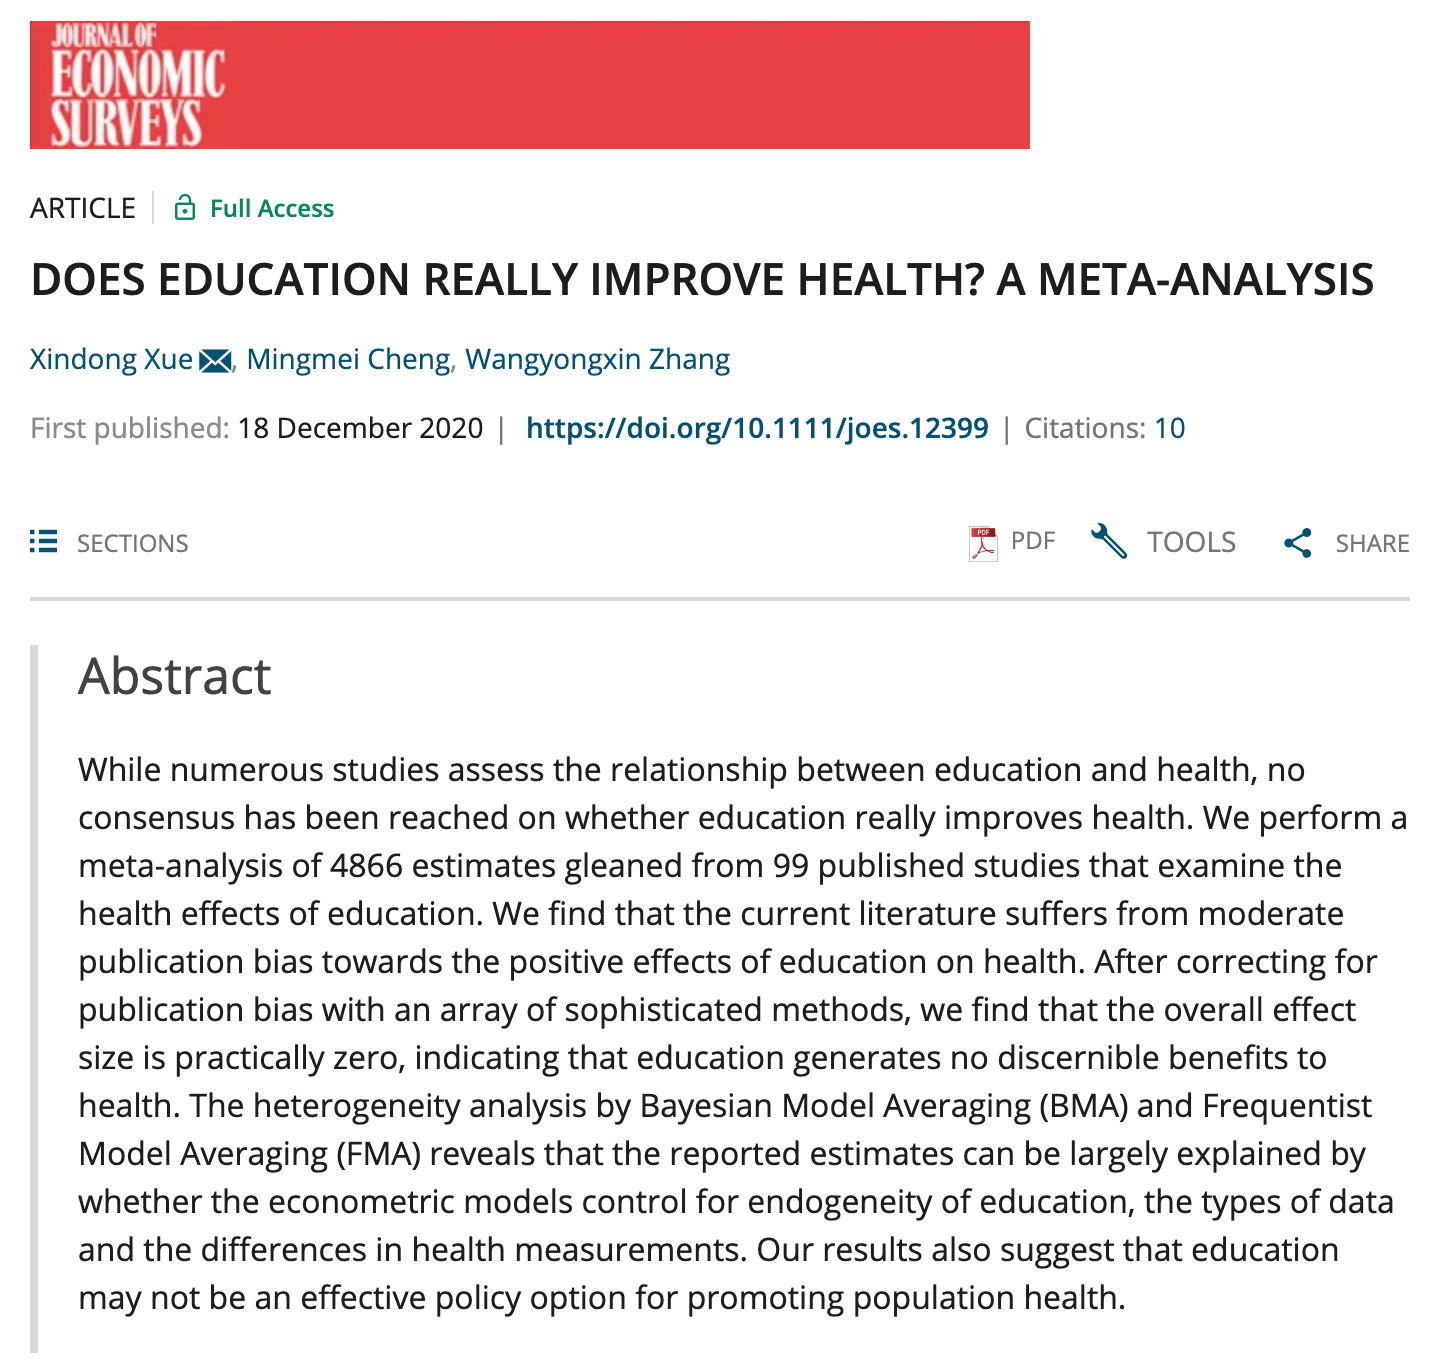
\includegraphics[width=3in]{images/ch3/49.png}
                \caption {Does education really improve health? A Meta-Analysis}
            \end{figure}

\begin{itemize}
    \item Publication bias towards the positive effects of education on health.
\end{itemize}

\subsubsection{Where Next?}
\begin{itemize}
    \item Grossman (NBER wp 21609, 2015) “The Relationship between Health and Schooling: What’s New?” concludes “There is enough conflicting evidence in the studies that I have reviewed to warrant more research on the question of whether more schooling does in fact cause better health outcomes.”
    \item Among promising areas of current and future research:
    \begin{itemize}
    \item Does schooling quality matter?
    \item What are the mechanisms via which schooling influences health and health behaviours?
    \item What is the role of genes?
    \item What is the role of subjective expectations of returns?
    \end{itemize}
\end{itemize}


\section*{Bibliography}

    \begin{itemize}
        \item Barcellos et al. (2018). PNAS. Education can reduce health differences related to genetic risk of obesity.
        \item Clark, D. and Royer, H. (2013). The Effect of Education on Adult Mortality: Evidence from Britain. American Economic Review, 106(6),
        2087-2120.
        \item Conti, G., and Hansman, C. (2013). Personality and the education–health gradient: A note on “Understanding differences in health
        behaviours by education”. Journal of health economics, 32(2), 480-485.
        \item Conti, G. and Heckman, J.J. (2010). Understanding the Early Origins of the Education-Health Gradient: A Framework That Can Also Be Applied to Analyze Gene-Environment Interactions. Perspectives on Psychological Science, 5(5), 585-605.
        \item Conti,G., Heckman,J.J. and Urzua, S. (2010).The Education-Health Gradient. American Economic Review P P, 100(2), 234-238.
        \item Cutler, D. M., and Lleras-Muney, A. (2010). Understanding differences in health behaviours by education. Journal of health economics,
        29(1), 1-28.
        • [Erlich, I., and H. Chuma (1990) “A model of the demand for longevity and the value of life extensions”, Journal of Political Economy
        98:761-782.]
        \item Galama,T. and H. van Kippersluis (2018).A Theory of Socioeconomic Disparities in Health Over the Life Cycle, Economic Journal.
        \item Galama, Titus J. and Lleras-Muney, Adriana and van Kippersluis, Hans, The Effect of Education on Health and Mortality: A Review of
        Experimental and Quasi-Experimental Evidence, Oxford Encyclopedia of Economics and Finance.
        \item Gilleskie, D. (2008). Health Capital: Theory and Empirical Evidence. Incentives and Choice in Health Care MIT Press: Cambridge, MA.
        \item Grossman, M. (1972). On the concept of health capital and the demand for health. Journal of Political economy, 80(2), 223-255.
        \item Grossman, M. (2000). The human capital model. Handbook of health economics, 1, 347-408.
        \item Grossman, M. (2015).The Relationship between Health and Schooling: What’s New? NBER wp 21609.
        \item Heckman, J. J. (2007). The economics, technology, and neuroscience of human capability formation. Proceedings of the national
        Academy of Sciences, 104(33), 13250-13255.
        \item Heckman, J.J., J.E. Humphries and G. Veramendi (2018). Returns to Education: The Causal Effects of Education on Earnings, Health
        and Smoking. Journal of Political Economy, October S1.
        \item Janke, K., D.Johnston, C. Propper and M. Shields (2018).The Causal Effect of Education on Chronic Health Conditions. IZA DP 11353.
        \item Lleras-Muney, A. (2005). The relationship between education and adult mortality in the United States. The Review of Economic
        Studies, 72(1), 189-221.
        \item Lundborg, P. (2013).The health returns to schooling—what can we learn from twins? Journal of population economics, 26(2), 673-701 
    \end{itemize}